% Options for packages loaded elsewhere
\PassOptionsToPackage{unicode}{hyperref}
\PassOptionsToPackage{hyphens}{url}
%
\documentclass[
]{book}
\usepackage{amsmath,amssymb}
\usepackage{lmodern}
\usepackage{ifxetex,ifluatex}
\ifnum 0\ifxetex 1\fi\ifluatex 1\fi=0 % if pdftex
  \usepackage[T1]{fontenc}
  \usepackage[utf8]{inputenc}
  \usepackage{textcomp} % provide euro and other symbols
\else % if luatex or xetex
  \usepackage{unicode-math}
  \defaultfontfeatures{Scale=MatchLowercase}
  \defaultfontfeatures[\rmfamily]{Ligatures=TeX,Scale=1}
\fi
% Use upquote if available, for straight quotes in verbatim environments
\IfFileExists{upquote.sty}{\usepackage{upquote}}{}
\IfFileExists{microtype.sty}{% use microtype if available
  \usepackage[]{microtype}
  \UseMicrotypeSet[protrusion]{basicmath} % disable protrusion for tt fonts
}{}
\makeatletter
\@ifundefined{KOMAClassName}{% if non-KOMA class
  \IfFileExists{parskip.sty}{%
    \usepackage{parskip}
  }{% else
    \setlength{\parindent}{0pt}
    \setlength{\parskip}{6pt plus 2pt minus 1pt}}
}{% if KOMA class
  \KOMAoptions{parskip=half}}
\makeatother
\usepackage{xcolor}
\IfFileExists{xurl.sty}{\usepackage{xurl}}{} % add URL line breaks if available
\IfFileExists{bookmark.sty}{\usepackage{bookmark}}{\usepackage{hyperref}}
\hypersetup{
  pdftitle={Data Science for Biologists - 5023Y},
  pdfauthor={Philip Leftwich},
  hidelinks,
  pdfcreator={LaTeX via pandoc}}
\urlstyle{same} % disable monospaced font for URLs
\usepackage{color}
\usepackage{fancyvrb}
\newcommand{\VerbBar}{|}
\newcommand{\VERB}{\Verb[commandchars=\\\{\}]}
\DefineVerbatimEnvironment{Highlighting}{Verbatim}{commandchars=\\\{\}}
% Add ',fontsize=\small' for more characters per line
\usepackage{framed}
\definecolor{shadecolor}{RGB}{248,248,248}
\newenvironment{Shaded}{\begin{snugshade}}{\end{snugshade}}
\newcommand{\AlertTok}[1]{\textcolor[rgb]{0.94,0.16,0.16}{#1}}
\newcommand{\AnnotationTok}[1]{\textcolor[rgb]{0.56,0.35,0.01}{\textbf{\textit{#1}}}}
\newcommand{\AttributeTok}[1]{\textcolor[rgb]{0.77,0.63,0.00}{#1}}
\newcommand{\BaseNTok}[1]{\textcolor[rgb]{0.00,0.00,0.81}{#1}}
\newcommand{\BuiltInTok}[1]{#1}
\newcommand{\CharTok}[1]{\textcolor[rgb]{0.31,0.60,0.02}{#1}}
\newcommand{\CommentTok}[1]{\textcolor[rgb]{0.56,0.35,0.01}{\textit{#1}}}
\newcommand{\CommentVarTok}[1]{\textcolor[rgb]{0.56,0.35,0.01}{\textbf{\textit{#1}}}}
\newcommand{\ConstantTok}[1]{\textcolor[rgb]{0.00,0.00,0.00}{#1}}
\newcommand{\ControlFlowTok}[1]{\textcolor[rgb]{0.13,0.29,0.53}{\textbf{#1}}}
\newcommand{\DataTypeTok}[1]{\textcolor[rgb]{0.13,0.29,0.53}{#1}}
\newcommand{\DecValTok}[1]{\textcolor[rgb]{0.00,0.00,0.81}{#1}}
\newcommand{\DocumentationTok}[1]{\textcolor[rgb]{0.56,0.35,0.01}{\textbf{\textit{#1}}}}
\newcommand{\ErrorTok}[1]{\textcolor[rgb]{0.64,0.00,0.00}{\textbf{#1}}}
\newcommand{\ExtensionTok}[1]{#1}
\newcommand{\FloatTok}[1]{\textcolor[rgb]{0.00,0.00,0.81}{#1}}
\newcommand{\FunctionTok}[1]{\textcolor[rgb]{0.00,0.00,0.00}{#1}}
\newcommand{\ImportTok}[1]{#1}
\newcommand{\InformationTok}[1]{\textcolor[rgb]{0.56,0.35,0.01}{\textbf{\textit{#1}}}}
\newcommand{\KeywordTok}[1]{\textcolor[rgb]{0.13,0.29,0.53}{\textbf{#1}}}
\newcommand{\NormalTok}[1]{#1}
\newcommand{\OperatorTok}[1]{\textcolor[rgb]{0.81,0.36,0.00}{\textbf{#1}}}
\newcommand{\OtherTok}[1]{\textcolor[rgb]{0.56,0.35,0.01}{#1}}
\newcommand{\PreprocessorTok}[1]{\textcolor[rgb]{0.56,0.35,0.01}{\textit{#1}}}
\newcommand{\RegionMarkerTok}[1]{#1}
\newcommand{\SpecialCharTok}[1]{\textcolor[rgb]{0.00,0.00,0.00}{#1}}
\newcommand{\SpecialStringTok}[1]{\textcolor[rgb]{0.31,0.60,0.02}{#1}}
\newcommand{\StringTok}[1]{\textcolor[rgb]{0.31,0.60,0.02}{#1}}
\newcommand{\VariableTok}[1]{\textcolor[rgb]{0.00,0.00,0.00}{#1}}
\newcommand{\VerbatimStringTok}[1]{\textcolor[rgb]{0.31,0.60,0.02}{#1}}
\newcommand{\WarningTok}[1]{\textcolor[rgb]{0.56,0.35,0.01}{\textbf{\textit{#1}}}}
\usepackage{longtable,booktabs,array}
\usepackage{calc} % for calculating minipage widths
% Correct order of tables after \paragraph or \subparagraph
\usepackage{etoolbox}
\makeatletter
\patchcmd\longtable{\par}{\if@noskipsec\mbox{}\fi\par}{}{}
\makeatother
% Allow footnotes in longtable head/foot
\IfFileExists{footnotehyper.sty}{\usepackage{footnotehyper}}{\usepackage{footnote}}
\makesavenoteenv{longtable}
\usepackage{graphicx}
\makeatletter
\def\maxwidth{\ifdim\Gin@nat@width>\linewidth\linewidth\else\Gin@nat@width\fi}
\def\maxheight{\ifdim\Gin@nat@height>\textheight\textheight\else\Gin@nat@height\fi}
\makeatother
% Scale images if necessary, so that they will not overflow the page
% margins by default, and it is still possible to overwrite the defaults
% using explicit options in \includegraphics[width, height, ...]{}
\setkeys{Gin}{width=\maxwidth,height=\maxheight,keepaspectratio}
% Set default figure placement to htbp
\makeatletter
\def\fps@figure{htbp}
\makeatother
\setlength{\emergencystretch}{3em} % prevent overfull lines
\providecommand{\tightlist}{%
  \setlength{\itemsep}{0pt}\setlength{\parskip}{0pt}}
\setcounter{secnumdepth}{5}
\usepackage{booktabs}
\usepackage{amsthm}
\makeatletter

\newenvironment{kframe}{%
\medskip{}
\setlength{\fboxsep}{.8em}
 \def\at@end@of@kframe{}%
 \ifinner\ifhmode%
  \def\at@end@of@kframe{\end{minipage}}%
  \begin{minipage}{\columnwidth}%
 \fi\fi%
 \def\FrameCommand##1{\hskip\@totalleftmargin \hskip-\fboxsep
 \colorbox{shadecolor}{##1}\hskip-\fboxsep
     % There is no \\@totalrightmargin, so:
     \hskip-\linewidth \hskip-\@totalleftmargin \hskip\columnwidth}%
 \MakeFramed {\advance\hsize-\width
   \@totalleftmargin\z@ \linewidth\hsize
   \@setminipage}}%
 {\par\unskip\endMakeFramed%
 \at@end@of@kframe}
\makeatother

\makeatletter
\@ifundefined{Shaded}{
}{\renewenvironment{Shaded}{\begin{kframe}}{\end{kframe}}}
\makeatother

\newenvironment{block}[1]
  {
  \begin{itemize}
  \renewcommand{\labelitemi}{
    \raisebox{-.7\height}[0pt][0pt]{
      {\setkeys{Gin}{width=3em,keepaspectratio}\includegraphics{images/#1}}
    }
  }
  \setlength{\fboxsep}{1em}
  \begin{kframe}
  \item
  }
  {
  \end{kframe}
  \end{itemize}
  }
\newenvironment{rmdnote}
  {\begin{block}{note}}
  {\end{block}}
\newenvironment{rmdtip}
  {\begin{block}{tip}}
  {\end{block}}
\newenvironment{rmdquestion}
  {\begin{block}{question}}
  {\end{block}}
\newenvironment{rmdwarning}
  {\begin{block}{warning}}
  {\end{block}}
  
\def\thm@space@setup{%
  \thm@preskip=8pt plus 2pt minus 4pt
  \thm@postskip=\thm@preskip
}
\makeatother
\ifluatex
  \usepackage{selnolig}  % disable illegal ligatures
\fi
\usepackage[]{natbib}
\bibliographystyle{apalike}

\title{Data Science for Biologists - 5023Y}
\author{Philip Leftwich}
\date{2021-10-02}

\begin{document}
\maketitle

{
\setcounter{tocdepth}{1}
\tableofcontents
}
\hypertarget{introduction}{%
\chapter{Introduction}\label{introduction}}

\hypertarget{approach-and-style}{%
\section{Approach and style}\label{approach-and-style}}

This book is designed to accompany the module BIO-5023Y for those new to R looking for best practices and tips. So it must be both accessible and succinct. The approach here is to provide just enough text explanation that someone very new to R can apply the code and follow what the code is doing. It is not a comprehensive textbook.

A few other points:

This is a code reference book accompanied by relatively brief examples - not a thorough textbook on R or data science

This is intended to be a living document - optimal R packages for a given task change often and we welcome discussion about which to emphasize in this handbook

Top tips for the course:

\textbf{DON'T} worry if you don't understand everything

\textbf{DO} ask lots of questions!

\hypertarget{teaching}{%
\section{Teaching}\label{teaching}}

We have:

\begin{itemize}
\tightlist
\item
  one lecture per week
\item
  one workshop per week
\end{itemize}

These are both timetabled in-person sessions, and you should check \href{https://timetabler.uea.ac.uk/Timetable}{Timetabler} for up to-date information on scheduling. However, all lessons can be accessed remotely through Collaborate, and \textbf{everything} you need to complete workshops will be available on this site.

If you feel unwell, or cannot attend a session in-person because you need to self-isolate then don't worry you can access everything, and follow along in real time, or work at your own pace.

Questions/issues/errors can all be posted on our \href{https://web.yammer.com/main/groups/eyJfdHlwZSI6Ikdyb3VwIiwiaWQiOiI3OTAyMTk1NzEyMCJ9/all}{Yammer} page.

\hypertarget{workshops}{%
\subsection{Workshops}\label{workshops}}

The workshops are the best way to learn, they teach you the practical skills you need to become an R wizard

\begin{figure}
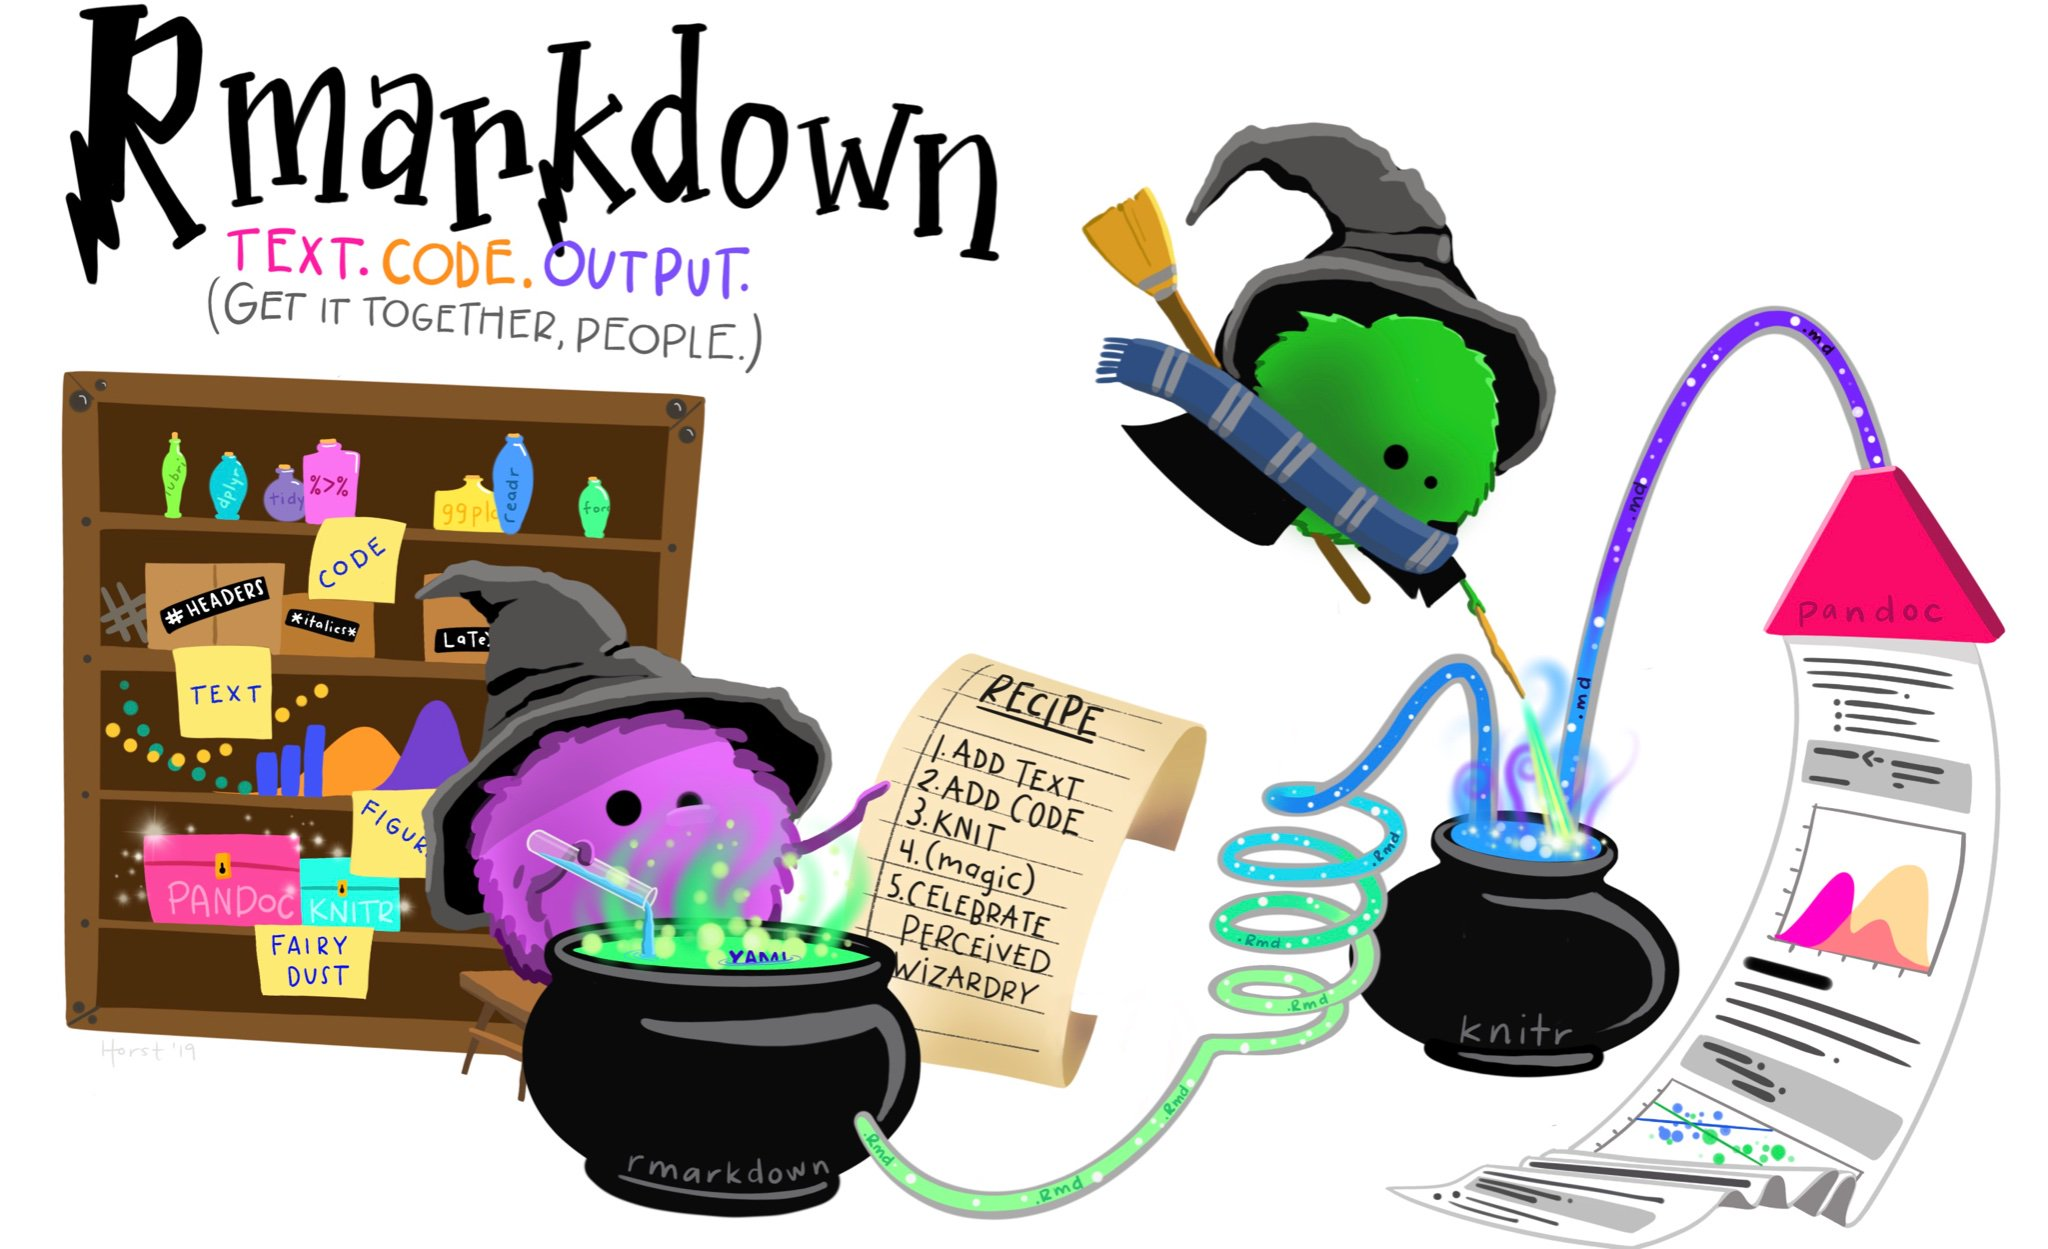
\includegraphics[width=0.8\linewidth]{images/wizard} \caption{courtesy of Allison Horst}\label{fig:unnamed-chunk-2}
\end{figure}

\hypertarget{introduction-to-r}{%
\section{Introduction to R}\label{introduction-to-r}}

\href{https://www.r-project.org/}{R} is the name of the programming language itself and \href{img/rstudio-ide.pdf}{RStudio} is a convenient interface.{]}, which we will be using throughout the course in order to learn how to organise data, produce accurate data analyses \& data visualisations.

Eventually we will also add extra tools like \href{https://www.youtube.com/watch?v=w3jLJU7DT5E}{GitHub} and \href{https://rmarkdown.rstudio.com/}{RMarkdown} for data reproducibility and collaborative programming, check out this short (and very cheesy) intro video.{]}, which are collaboration and version control systems that we will be using throughout the course. More on this in future weeks.

By the end of this module I hope you will have the tools to confidently analyze real data, make informative and beautiful data visuals, and be able to analyse lots of different types of data.

The taught content this autumn will be given to you in several \textbf{worksheets}, these will be added to this dynamic webpage each week.

\hypertarget{getting-around-on-rstudio}{%
\section{Getting around on RStudio}\label{getting-around-on-rstudio}}

All of our sessions will run on cloud-based software. All you have to do is make a free account, and join our Workspace \texttt{BIO-5023Y} the sharing link is \href{https://rstudio.cloud/spaces/84058/join?access_code=6c3uEkEUsNhbzUrttMcRq3SoSkQ4vKw\%2FeYBoyBRu}{here}.

Once you are signed up - you will see that there are two \texttt{Spaces}

\begin{itemize}
\item
  Your workspace
\item
  BIO-5023Y
\end{itemize}

Make sure you are working in the class workspace - there is a limit to the hours/month on your workspace, so all assigments and project work should take place in the \texttt{BIO-5023Y\ space}.

Watch these short explainer videos to get used to navigating the environment.

\hypertarget{an-intro-to-rstudio}{%
\subsection{An intro to RStudio}\label{an-intro-to-rstudio}}

RStudio

\begin{quote}
Note - people often mix up R and RStudio. R is the programming language (the engine), RStudio is a handy interface/wrapper that makes things a bit easier to use.
\end{quote}

\hypertarget{using-r-studio-cloud}{%
\subsection{Using R Studio Cloud}\label{using-r-studio-cloud}}

RStudio Cloud works in exactly the same way as RStudio, but means you don't have to download any software. You can access the hosted cloud server and your projects through any browser connection (Chrome works best), from any computer.

\hypertarget{reading}{%
\section{Reading}\label{reading}}

There are lots of useful books and online resources to help develop and improve your R knowledge. Throughout this webpage I will be adding useful resources for you.

The core textbook you might want to bookmark is R for Data Science \citep{R4DS} but we will add others throughout the course, and their is a bibliography at the end which collects everything together!

\hypertarget{get-help}{%
\section{Get Help!}\label{get-help}}

There are a \textbf{lot} of sources of information about using R out there.
Here are a few helpful places to get help when you have an issue, or just to learn more

\begin{itemize}
\item
  The R help system itself - we cover this in Week one \protect\hyperlink{error}{Error}
\item
  Vignettes - type \texttt{browseVignettes()} into the console and hit Enter, a list of available vignettes for all the packages we have will be displayed
\item
  \href{https://www.rstudio.com/resources/cheatsheets/}{Cheat Sheets} - available at RStudio.com. Most common packages have an associate cheat sheet covering the basics of how to use them. Download/bookmark ones we will use commonly such as \texttt{ggplot2}, \texttt{Data\ transformation\ with\ dplyr}, \texttt{Data\ tidying\ with\ tidyr} \& \texttt{Data\ import}.
\item
  Google - I use Google constantly, because I continually forget how to do even basic tasks. If I want to remind myself how to round a number, I might type something like \texttt{R\ round\ number} - if I am using a particular package I should include that in the search term as well
\item
  \href{https://web.yammer.com/main/groups/eyJfdHlwZSI6Ikdyb3VwIiwiaWQiOiI3OTAyMTk1NzEyMCJ9/all}{Ask for help} - If you are stuck, getting an error message, can't think what to do next, then ask someone. It could be me, it could be a classmate. When you do this it is very important that you \textbf{show the code}, include the \textbf{error message}. ``This doesn't work'' is not helpful. ``Here is my code, this is the data I am using, I want it to do X, and here's the problem I get''.
\end{itemize}

\begin{quote}
Note - It may be daunting to send your code to someone for help. It is natural and common to feel apprehensive, or to think that your code is really bad. I still feel the same! But we learn when we share our mistakes, and eventually you will find it funny when you look back on your early mistakes, or laugh about the mistakes you still occasionally make!
\end{quote}

\hypertarget{getting-to-know-r---week-one}{%
\chapter{Getting to know R - Week One}\label{getting-to-know-r---week-one}}

Go to RStudio Cloud and enter the Project labelled \texttt{Week\ One} - this will clone the project and provide you with your own workspace.

Follow the instructions below to get used to the R command line, and how R works as a language.

\hypertarget{your-first-r-command}{%
\section{Your first R command}\label{your-first-r-command}}

In the RStudio pane, navigate to the console (bottom left) and \texttt{type\ or\ copy} the below it should appear at the \textgreater{}

Hit Enter on your keyboard.

\begin{Shaded}
\begin{Highlighting}[]
\DecValTok{10} \SpecialCharTok{+} \DecValTok{20}
\end{Highlighting}
\end{Shaded}

You should now be looking at the below:

\begin{verbatim}
> 10 + 20
[1] 30
\end{verbatim}

The first line shows the request you made to R, the next line is R's response

You didn't type the \texttt{\textgreater{}} symbol: that's just the R command prompt and isn't part of the actual command.

It's important to understand how the output is formatted. Obviously, the correct answer to the sum \texttt{10\ +\ 20} is \texttt{30}, and not surprisingly R has printed that out as part of its response. But it's also printed out this \texttt{{[}1{]}} part, which probably doesn't make a lot of sense to you right now. You're going to see that a lot. You can think of \texttt{{[}1{]}\ 30} as if R were saying ``the answer to the 1st question you asked is 30''.

\hypertarget{typos}{%
\subsection{Typos}\label{typos}}

Before we go on to talk about other types of calculations that we can do with R, there's a few other things I want to point out. The first thing is that, while R is good software, it's still software. It's pretty stupid, and because it's stupid it can't handle typos. It takes it on faith that you meant to type \emph{exactly} what you did type. For example, suppose that you forgot to hit the shift key when trying to type \texttt{+}, and as a result your command ended up being \texttt{10\ =\ 20} rather than \texttt{10\ +\ 20}. Try it for yourself and replicate this error message:

\begin{Shaded}
\begin{Highlighting}[]
\DecValTok{10} \OtherTok{=} \DecValTok{20}
\end{Highlighting}
\end{Shaded}

\begin{verbatim}
## Error in 10 = 20: invalid (do_set) left-hand side to assignment
\end{verbatim}

What's happened here is that R has attempted to interpret \texttt{10\ =\ 20} as a command, and spits out an error message because the command doesn't make any sense to it. When a \emph{human} looks at this, and then looks down at his or her keyboard and sees that \texttt{+} and \texttt{=} are on the same key, it's pretty obvious that the command was a typo. But R doesn't know this, so it gets upset. And, if you look at it from its perspective, this makes sense. All that R ``knows'' is that \texttt{10} is a legitimate number, \texttt{20} is a legitimate number, and \texttt{=} is a legitimate part of the language too. In other words, from its perspective this really does look like the user meant to type \texttt{10\ =\ 20}, since all the individual parts of that statement are legitimate and it's too stupid to realise that this is probably a typo. Therefore, R takes it on faith that this is exactly what you meant\ldots{} it only ``discovers'' that the command is nonsense when it tries to follow your instructions, typo and all. And then it whinges, and spits out an error.

Even more subtle is the fact that some typos won't produce errors at all, because they happen to correspond to ``well-formed'' R commands. For instance, suppose that not only did I forget to hit the shift key when trying to type \texttt{10\ +\ 20}, I also managed to press the key next to one I meant do. The resulting typo would produce the command \texttt{10\ -\ 20}. Clearly, R has no way of knowing that you meant to \emph{add} 20 to 10, not \emph{subtract} 20 from 10, so what happens this time is this:

\begin{Shaded}
\begin{Highlighting}[]
\DecValTok{10} \SpecialCharTok{{-}} \DecValTok{20}
\end{Highlighting}
\end{Shaded}

\begin{verbatim}
## [1] -10
\end{verbatim}

In this case, R produces the right answer, but to the the wrong question.

\hypertarget{more-simple-arithmetic}{%
\subsection{More simple arithmetic}\label{more-simple-arithmetic}}

One of the best ways to get to know R is to play with it, it's pretty difficult to break it so don't worry too much. Type whatever you want into to the console and see what happens.

If the last line of your console looks like this

\begin{verbatim}
> 10+
+ 
\end{verbatim}

and there's a blinking cursor next to the plus sign. This means is that R is still waiting for you to finish. It ``thinks'' you're still typing your command, so it hasn't tried to execute it yet. In other words, this plus sign is actually another command prompt. It's different from the usual one (i.e., the \texttt{\textgreater{}} symbol) to remind you that R is going to ``add'' whatever you type now to what you typed last time. For example, type \texttt{20} and hit enter, then it finishes the command:

\begin{verbatim}
> 10 +
+ 20
[1] 30
\end{verbatim}

\emph{Alternatively} hit escape, and R will forget what you were trying to do and return to a blank line.

\hypertarget{try-some-maths}{%
\subsection{Try some maths}\label{try-some-maths}}

\begin{Shaded}
\begin{Highlighting}[]
\DecValTok{1}\SpecialCharTok{+}\DecValTok{7}
\end{Highlighting}
\end{Shaded}

\begin{Shaded}
\begin{Highlighting}[]
\DecValTok{13{-}10}
\end{Highlighting}
\end{Shaded}

\begin{Shaded}
\begin{Highlighting}[]
\DecValTok{4}\SpecialCharTok{*}\DecValTok{6}
\end{Highlighting}
\end{Shaded}

\begin{Shaded}
\begin{Highlighting}[]
\DecValTok{12}\SpecialCharTok{/}\DecValTok{3}
\end{Highlighting}
\end{Shaded}

Raise a number to the power of another

\begin{Shaded}
\begin{Highlighting}[]
\DecValTok{5}\SpecialCharTok{\^{}}\DecValTok{4}
\end{Highlighting}
\end{Shaded}

As I'm sure everyone will probably remember the moment they read this, the act of multiplying a number \(x\) by itself \(n\) times is called ``raising \(x\) to the \(n\)-th power''. Mathematically, this is written as \(x^n\). Some values of \(n\) have special names: in particular \(x^2\) is called \(x\)-squared, and \(x^3\) is called \(x\)-cubed. So, the 4th power of 5 is calculated like this:
\[
5^4 = 5 \times 5 \times 5 \times 5 
\]

\hypertarget{perform-some-combos}{%
\subsection{Perform some combos}\label{perform-some-combos}}

Perform some mathematical combos, noting that the order in which R performs calculations is the standard one.

That is, first calculate things inside \textbf{B}rackets \texttt{()}, then calculate \textbf{O}rders of (exponents) \texttt{\^{}}, then \textbf{D}ivision \texttt{/} and \textbf{M}ultiplication \texttt{*}, then \textbf{A}ddition \texttt{+} and \textbf{S}ubtraction \texttt{-}.

Notice the different outputs of these two commands.

\begin{Shaded}
\begin{Highlighting}[]
\DecValTok{3}\SpecialCharTok{\^{}}\DecValTok{2{-}5}\SpecialCharTok{/}\DecValTok{2}
\end{Highlighting}
\end{Shaded}

\begin{Shaded}
\begin{Highlighting}[]
\NormalTok{(}\DecValTok{3}\SpecialCharTok{\^{}}\DecValTok{2{-}5}\NormalTok{)}\SpecialCharTok{/}\DecValTok{2}
\end{Highlighting}
\end{Shaded}

Similarly if we want to raise a number to a fraction, we need to surround the fraction with parentheses ()

\begin{Shaded}
\begin{Highlighting}[]
\DecValTok{16}\SpecialCharTok{\^{}}\DecValTok{1}\SpecialCharTok{/}\DecValTok{2}
\end{Highlighting}
\end{Shaded}

\begin{Shaded}
\begin{Highlighting}[]
\DecValTok{16}\SpecialCharTok{\^{}}\NormalTok{(}\DecValTok{1}\SpecialCharTok{/}\DecValTok{2}\NormalTok{)}
\end{Highlighting}
\end{Shaded}

The first one calculates 16 raised to the power of 1, then divided this answer by two. The second one raises 16 to the power of a half. A big difference in the output.

\begin{quote}
**Note - While the cursor is in the console, you can press the up arrow to see all your previous commands.
You can run them again, or edit them. Later on we will look at scripts, as an essential way to re-use, store and edit commands.
\end{quote}

\hypertarget{true-or-false-data}{%
\section{``true or false'' data}\label{true-or-false-data}}

Time to make a sidebar onto another kind of data. A key concept in that a lot of R relies on is the idea of a \textbf{\emph{logical value}}. A logical value is an assertion about whether something is true or false. This is implemented in R in a pretty straightforward way. There are two logical values, namely \texttt{TRUE} and \texttt{FALSE}. Despite the simplicity, a logical values are very useful things. Let's see how they work.

\hypertarget{assessing-mathematical-truths}{%
\subsection{Assessing mathematical truths}\label{assessing-mathematical-truths}}

In George Orwell's classic book \emph{1984}, one of the slogans used by the totalitarian Party was ``two plus two equals five'', the idea being that the political domination of human freedom becomes complete when it is possible to subvert even the most basic of truths.

But they didn't have R. R will not be subverted. It has rather firm opinions on the topic of what is and isn't true, at least as regards basic mathematics. If I ask it to calculate \texttt{2\ +\ 2}, it always gives the same answer, and it's not bloody 5:

\begin{Shaded}
\begin{Highlighting}[]
\DecValTok{2} \SpecialCharTok{+} \DecValTok{2}
\end{Highlighting}
\end{Shaded}

Of course, so far R is just doing the calculations. I haven't asked it to explicitly assert that \(2+2 = 4\) is a true statement. If I want R to make an explicit judgement, I can use a command like this:

\begin{Shaded}
\begin{Highlighting}[]
\DecValTok{2} \SpecialCharTok{+} \DecValTok{2} \SpecialCharTok{==} \DecValTok{4}
\end{Highlighting}
\end{Shaded}

What I've done here is use the \textbf{\emph{equality operator}}, \texttt{==}, to force R to make a ``true or false'' judgement.

\begin{quote}
**Note that this is a very different operator to the assignment operator \texttt{=} you saw previously. A common typo that people make when trying to write logical commands in R (or other languages, since the ``\texttt{=} versus \texttt{==}'' distinction is important in most programming languages) is to accidentally type \texttt{=} when you really mean \texttt{==}.
\end{quote}

Okay, let's see what R thinks of the Party slogan:

\begin{Shaded}
\begin{Highlighting}[]
\DecValTok{2}\SpecialCharTok{+}\DecValTok{2} \SpecialCharTok{==} \DecValTok{5}
\end{Highlighting}
\end{Shaded}

Take that Big Brother! Anyway, it's worth having a look at what happens if I try to \emph{force} R to believe that two plus two is five by making an assignment statement like \texttt{2\ +\ 2\ =\ 5} or \texttt{2\ +\ 2\ \textless{}-\ 5}. When I do this, here's what happens:

\begin{Shaded}
\begin{Highlighting}[]
\DecValTok{2} \SpecialCharTok{+} \DecValTok{2} \OtherTok{=} \DecValTok{5}
\end{Highlighting}
\end{Shaded}

R doesn't like this very much. It recognises that \texttt{2\ +\ 2} is \emph{not} a variable (that's what the ``non-language object'' part is saying), and it won't let you try to ``reassign'' it. While R is pretty flexible, and actually does let you do some quite remarkable things to redefine parts of R itself, there are just some basic, primitive truths that it refuses to give up. It won't change the laws of addition, and it won't change the definition of the number \texttt{2}.

That's probably for the best.

\hypertarget{storing-outputs}{%
\section{Storing outputs}\label{storing-outputs}}

With simple questions like the ones above we are happy to just see the answer, but our quesitons are often more complex than this. If we need to take multiple steps, we benefit from being able to store our answers and recall them for use in later steps. This is very simple to do we can \emph{assign} outputs to a name:

\begin{Shaded}
\begin{Highlighting}[]
\NormalTok{a }\OtherTok{\textless{}{-}} \DecValTok{1}\SpecialCharTok{+}\DecValTok{2}
\end{Highlighting}
\end{Shaded}

This literally means please \emph{assign} the value of \texttt{1+2} to the name \texttt{a}. We use the \textbf{assignment operator} \texttt{\textless{}-} to make this assignment.

\begin{quote}
**Note the shortcut key for \textless- is Alt + - (Windows) or Option + - (Mac)
\end{quote}

If you perform this action you should be able to do two things

\begin{itemize}
\item
  You should be able to see that in the top right-hand pane in the \texttt{Environment} tab their is now an \texttt{object} called a with the value of 3.
\item
  You should be able to look at what a is by typing it into your Console and pressing Enter
\end{itemize}

\begin{Shaded}
\begin{Highlighting}[]
\NormalTok{a}
\end{Highlighting}
\end{Shaded}

\begin{verbatim}
> a
[1] 3
\end{verbatim}

You can now call this object at any time during your R session and perform calculations with it.

\begin{Shaded}
\begin{Highlighting}[]
\DecValTok{2} \SpecialCharTok{*}\NormalTok{ a}
\end{Highlighting}
\end{Shaded}

\begin{verbatim}
[1] 6
\end{verbatim}

What happens if we assign a value to a named object that already exists in our R environment??? for example

\begin{Shaded}
\begin{Highlighting}[]
\NormalTok{a }\OtherTok{\textless{}{-}} \DecValTok{10}
\NormalTok{a}
\end{Highlighting}
\end{Shaded}

\begin{verbatim}
[1] 10
\end{verbatim}

You should see that the previous assignment is lost, \emph{gone forever} and has been replaced by the new value.

We can assign lots of things to objects, and use them in calculations to build more objects.

\begin{Shaded}
\begin{Highlighting}[]
\NormalTok{b }\OtherTok{\textless{}{-}} \DecValTok{5}
\NormalTok{c }\OtherTok{\textless{}{-}}\NormalTok{ a }\SpecialCharTok{+}\NormalTok{ b}
\end{Highlighting}
\end{Shaded}

Note that if you now change the value of b, the value of c does \emph{not} change. Objects are totally independent from each other once they are made

\begin{Shaded}
\begin{Highlighting}[]
\NormalTok{b }\OtherTok{\textless{}{-}} \DecValTok{7}
\NormalTok{b}
\NormalTok{c}
\end{Highlighting}
\end{Shaded}

Look at the environment tab again - you should see it's starting to fill up now!

\begin{quote}
**Note - RStudio will by default save the objects in its memory when you close a session. These will then be there the next time you logon. It might seem nice to be able to close things down and pick up where you left off, but its actually quite dangerous. It's messy, and can cause lots of problems when we work with scripts later, so don't do this!!! To stop RStudio from saving objects by default go to the Preferences option and change ``Save workspace to .RData on exit'' to ``Never''. Instead we are going to learn how to use scripts to quickly re-run analyses we have been working on.
\end{quote}

\hypertarget{choosing-names}{%
\subsection{Choosing names}\label{choosing-names}}

\begin{itemize}
\item
  Use informative variable names. As a general rule, using meaningful names like \texttt{orange} and \texttt{apple} is preferred over arbitrary ones like \texttt{variable1} and \texttt{variable2}. Otherwise it's very hard to remember what the contents of different variables actually are.
\item
  Use short variable names. Typing is a pain and no-one likes doing it. So we much prefer to use a name like \texttt{apple} over a name like \texttt{pink\_lady\_apple}.
\item
  Use one of the conventional naming styles for multi-word variable names. R only lets you use certain things as \textbf{legal} names. Legal names must start with a letter \textbf{not} a number, which can then be followed by a sequence of letters, numbers, ., or \_. R does not like using spaces. Upper and lower case names are allowed, but R is case sensitive so \texttt{Apple} and \texttt{apple} are different.
\item
  My favourite naming convention is \texttt{snake\_case} short, lower case only, spaces between words are separated with a \_. It's easy to read and easy to remember.
\end{itemize}

\hypertarget{writing-scripts}{%
\section{Writing scripts}\label{writing-scripts}}

Until now we have been typing words directly into the Console. This is fine for short/simple calculations - but as soon as we have a more complex, multi-step process this becomes time consuming, error-prone and \emph{boring}. \textbf{Scripts} are a document containing all of your commands (in the order you want them to run), they are \emph{repeatable, shareable, annotated records of what you have done}. In short they are incredibly useful - and a big step towards \textbf{open} and \textbf{reproducible} research.

To create a script go to File \textgreater{} New File \textgreater{} R Script.

This will open a pane in the top-left of RStudio with a tab name of \texttt{Untitled1}. In your new script, type some of the basic arithmetic and assignment commands you used previously. When you write a script, make sure it has all of the commands you need to complete your analysis, \emph{in the order you want them to run}.

\hypertarget{commenting-on-scripts}{%
\subsection{Commenting on scripts}\label{commenting-on-scripts}}

Annotating your instructions provides yourself and others insights into why you are doing what you are doing. This is a vital aspect of a robust and reproducible workflow. And when you come back to a script, one week, one month or one year from now you will often wonder what a command was for. It is very, very useful to make notes for yourself, and its useful in case anyone else will ever read your script. Make these comments helpful they are for humans to read.

In R we signal a comment with the \# key. Everything in the line after a \# is ignored by R and won't be treated as a command. You should see that it is marked in a different colour in your script.

Put the following comment in your script. Try adding a few comments to your previous lines of code

\begin{Shaded}
\begin{Highlighting}[]
\CommentTok{\# I really love R}
\end{Highlighting}
\end{Shaded}

\hypertarget{running-your-script}{%
\subsection{Running your script}\label{running-your-script}}

To run the commands from your script, we need to get it into the Console. You could select and copy/paste this into the Console. But there are a couple of faster shortcuts.

\begin{itemize}
\item
  Hit the Run button in the top right of the script pane. Pressing this will run the line of code the cursor is sitting on.
\item
  Pressing Ctrl+Enter will do the same thing as hitting the Run button
\item
  If you want to run the whole script in one go then press Ctrl+A then either click Run or press Ctrl+Enter
\end{itemize}

\hypertarget{saving-your-script}{%
\subsection{Saving your script}\label{saving-your-script}}

Our script now contains code and comments from our first workshop. We need to save it.

Alongside our data, our script is the most precious part of our analysis. We don't need to save anything else, any outputs etc. because our script can always be used to generate everything again. Note the colour of the script - the name changes colour when we have unsaved changes. Press the Save button or go to File \textgreater{} Save as.
Give the File a sensible name like ``Simple commands in R'' and in the bottom right pane under \texttt{Files} you should now be able to see your saved script.

You could now safely quit R, and when you log on next time to this project, your script will be waiting for you.

\hypertarget{error}{%
\section{Error}\label{error}}

Things will go wrong eventually, they always do\ldots{}

R is \emph{very} pedantic, even the smallest typo can result in failure and typos are impossilbe to avoid. So we will make mistakes. One type of mistake we will make is an \textbf{error}. The code fails to run. The most common causes for an error are:

\begin{itemize}
\item
  typos
\item
  missing commas
\item
  missing brackets
\end{itemize}

There's nothing wrong with making \emph{lots} of errors. The trick is not to panic or get frustrated, but to read the error message and our script carefully and start to \emph{debug}\ldots{}

\ldots{} and sometimes we need to walk away and come back later!

\begin{figure}

\includegraphics[width=0.8\linewidth]{images/Error} \caption{courtesy of Allison Horst}\label{fig:unnamed-chunk-28}
\end{figure}

\hypertarget{functions}{%
\section{Functions}\label{functions}}

Functions are the tools of R. Each one helps us to do a different task.

Take for example the function that we use to round a number to a certain number of digits - this function is called \texttt{round}

Here's an example

\begin{Shaded}
\begin{Highlighting}[]
\FunctionTok{round}\NormalTok{(}\AttributeTok{x  =} \FloatTok{2.4326782647}\NormalTok{, }\AttributeTok{digits =} \DecValTok{2}\NormalTok{)}
\end{Highlighting}
\end{Shaded}

We start the command with the function name \texttt{round}. The name is followed by parentheses (). Within these we place the \emph{arguments} for the function, each of which is separated by a comma.

The arguments

\begin{itemize}
\item
  x = 2.4326782647
\item
  digits = 2
\end{itemize}

Arguments are the information we give to a function. These arguments are in the form \texttt{name\ =\ value} the name specifies the argument, and the value is what we are providing. That is the first argument x is the number we would like to round, it has a value of 2.4326782647. The second argument digits is how we would like the number to be rounded and we specify 2.

Ok put the above commmand in your script and add a comment with \# as to what you are doing.

\hypertarget{storing-the-output-of-functions}{%
\subsection{Storing the output of functions}\label{storing-the-output-of-functions}}

What if we need the answer from a function in a later calculation. The answer is to use the assignment operator again.

Can you work out what is going on here? If so copy this into your R script and a \#comment next to each line.

\begin{Shaded}
\begin{Highlighting}[]
\NormalTok{number\_of\_digits }\OtherTok{\textless{}{-}} \DecValTok{2}
\NormalTok{my\_number }\OtherTok{\textless{}{-}} \FloatTok{2.4326782647}
\NormalTok{rounded\_number }\OtherTok{\textless{}{-}} \FunctionTok{round}\NormalTok{(}\AttributeTok{x  =}\NormalTok{ my\_number, }
                        \AttributeTok{digits =}\NormalTok{ number\_of\_digits)}
\end{Highlighting}
\end{Shaded}

\hypertarget{more-fun-with-functions}{%
\subsection{More fun with functions}\label{more-fun-with-functions}}

Check this out

\begin{Shaded}
\begin{Highlighting}[]
\FunctionTok{round}\NormalTok{(}\FloatTok{2.4326782647}\NormalTok{, }\DecValTok{2}\NormalTok{)}
\end{Highlighting}
\end{Shaded}

We don't \emph{have} to give the names of arguments for a function to still work. This works because the function \texttt{round} expects us to give the number value first, and the argument for rounding digits second. \emph{But} this assumes we know the expected ordering within a function, this might be the case for functions we use a lot. If you give arguments their proper names \emph{then} you can actually introduce them in any order you want.

Try this:

\begin{Shaded}
\begin{Highlighting}[]
\FunctionTok{round}\NormalTok{(}\AttributeTok{digits =} \DecValTok{2}\NormalTok{, }\AttributeTok{x  =} \FloatTok{2.4326782647}\NormalTok{)}
\end{Highlighting}
\end{Shaded}

But this gives a different answer

\begin{Shaded}
\begin{Highlighting}[]
\FunctionTok{round}\NormalTok{(}\DecValTok{2}\NormalTok{, }\FloatTok{2.4326782647}\NormalTok{)}
\end{Highlighting}
\end{Shaded}

Are you happy with what is happening here? naming arguments overrides the position defaults

Ok what about this?

\begin{Shaded}
\begin{Highlighting}[]
\FunctionTok{round}\NormalTok{(}\FloatTok{2.4326782647}\NormalTok{)}
\end{Highlighting}
\end{Shaded}

We didn't specify how many digits to round to, but we still got an answer. That's because in many functions arguments have \texttt{defaults} - the default argument here is digits = 0. So we don't have to specify the argument if we are happy for round to produce whole numbers.

How do we know argument orders and defaults? Well we get to know how a lot of functions work through practice, but we can also use the inbuilt R help. This is a function - but now we specify the name of another function to provide a help menu.

\begin{Shaded}
\begin{Highlighting}[]
\FunctionTok{help}\NormalTok{(round)}
\end{Highlighting}
\end{Shaded}

\hypertarget{packages}{%
\section{Packages}\label{packages}}

An R package is a container for various things including functions and data. These make it easy to do very complicate protocols by using custom-built functions. Later we will see how we can write our own simple functions.

On RStudio Cloud I have already installed several add-on packages, all we need to do is use a simple function to load these packages into our workspace. Once this is complete we will have access to all the custom functions they contain.

Let's try that now:

\begin{Shaded}
\begin{Highlighting}[]
\FunctionTok{library}\NormalTok{(ggplot2)}
\FunctionTok{library}\NormalTok{(palmerpenguins)}
\end{Highlighting}
\end{Shaded}

\begin{quote}
Errors part 2 Another common source of errors is to call a function that is part of a package but forgetting to load the package. If R says something like ``Error in function-name'' then most likely the function was misspelled or the package containing the function hasn't been loaded.
\end{quote}

Packages are a lot like new apps extending the functionality of what your phone can do. To use the functionalities of a package they must be loaded \emph{before} we call on the funcitons or data they contain. So the most sensible place to put library calls for packages is at the very \textbf{top} of our script. So let's do that now.

\hypertarget{my-first-data-visualisation}{%
\section{My first data visualisation}\label{my-first-data-visualisation}}

Let's run our first data visualisation using the functions and data we have now loaded - this produces a plot using functions from the \texttt{ggplot2} package (\citet{R-ggplot2}) and data from the \texttt{palmerpenguins} (\citet{R-palmerpenguins}) package. Use the \# comments to add notes on what you are using each package for in your script.

Using these functions we can write a simple line of code to produce a figure. We specify the data source, the variables to be used for the x and y axis and then the type of visual object to produce, colouring them by the species.

Copy this into your console and hit Enter.

\begin{Shaded}
\begin{Highlighting}[]
\FunctionTok{ggplot}\NormalTok{(}\AttributeTok{data =}\NormalTok{ penguins,}\FunctionTok{aes}\NormalTok{(}\AttributeTok{x =}\NormalTok{ bill\_length\_mm, }\AttributeTok{y =}\NormalTok{ bill\_depth\_mm)) }\SpecialCharTok{+} \FunctionTok{geom\_point}\NormalTok{(}\FunctionTok{aes}\NormalTok{(}\AttributeTok{colour=}\NormalTok{species)) }
\end{Highlighting}
\end{Shaded}

\begin{quote}
**Note - you may have noticed R gave you a warning. Not the same as a big scary error, but R wants you to be aware of something. In this case that two of the observations had missing data in them (either bill length or bill depth), so couldn't be plotted.
\end{quote}

The above command can also be written as below, its in a longer style with each new line for each argument in the function. This style can be easier to read, and makes it easier to write comments with \#. Copy this longer command into your \texttt{script} then run it by either highlighting the entire command or placing the cursor in the first line and then hit Run or Ctrl+Enter.

\begin{Shaded}
\begin{Highlighting}[]
\FunctionTok{ggplot}\NormalTok{(}\AttributeTok{data =}\NormalTok{ penguins, }\CommentTok{\# calls ggplot function, data is penguins}
       \FunctionTok{aes}\NormalTok{(}\AttributeTok{x =}\NormalTok{ bill\_length\_mm, }\CommentTok{\# sets x axis as bill length}
           \AttributeTok{y =}\NormalTok{ bill\_depth\_mm)) }\SpecialCharTok{+} \CommentTok{\# sets y axis value as bill depth}
    \FunctionTok{geom\_point}\NormalTok{(}\FunctionTok{aes}\NormalTok{(}\AttributeTok{colour=}\NormalTok{species)) }\CommentTok{\# plot points coloured by penguin species}
\end{Highlighting}
\end{Shaded}

\hypertarget{quitting}{%
\section{Quitting}\label{quitting}}

\begin{itemize}
\item
  Make sure you have saved any changes to your R script - that's all you need to make sure you've done!
\item
  If you want me to take a look at your script let me know
\item
  If you spotted any mistakes or errors let me know
\item
  Close your RStudio Cloud Browser
\item
  Go to Blackboard to complete a short quiz!
\end{itemize}

\hypertarget{workflow-part-one---week-two}{%
\chapter{Workflow Part One - Week Two}\label{workflow-part-one---week-two}}

Last week we got acquainted with some of the core skills associated with using R and RStudio.

In this workshop we work through the journey of importing and tidying data. Once we have a curated and cleaned dataset we can work on generating insights from the data.

We are going to be working as though we are in the latter stages of a research project, where data has been collected, possibly over several years, to test against our hypotheses.

We have chosen to continue working with a dataset you have been introduced to already - the Palmer Penguins dataset. Previously we loaded a cleaned dataset, very quickly using an R package. Today we will be working in a more realistic scenario - uploading out dataset to our R workspace.

\hypertarget{meet-the-penguins}{%
\section{Meet the Penguins}\label{meet-the-penguins}}

This data, taken from the \texttt{palmerpenguins} (\citet{R-palmerpenguins}) package was originally published by \citet{Antarctic}.

The palmerpenguins data contains size measurements, clutch observations, and blood isotope ratios for three penguin species observed on three islands in the Palmer Archipelago, Antarctica over a study period of three years.

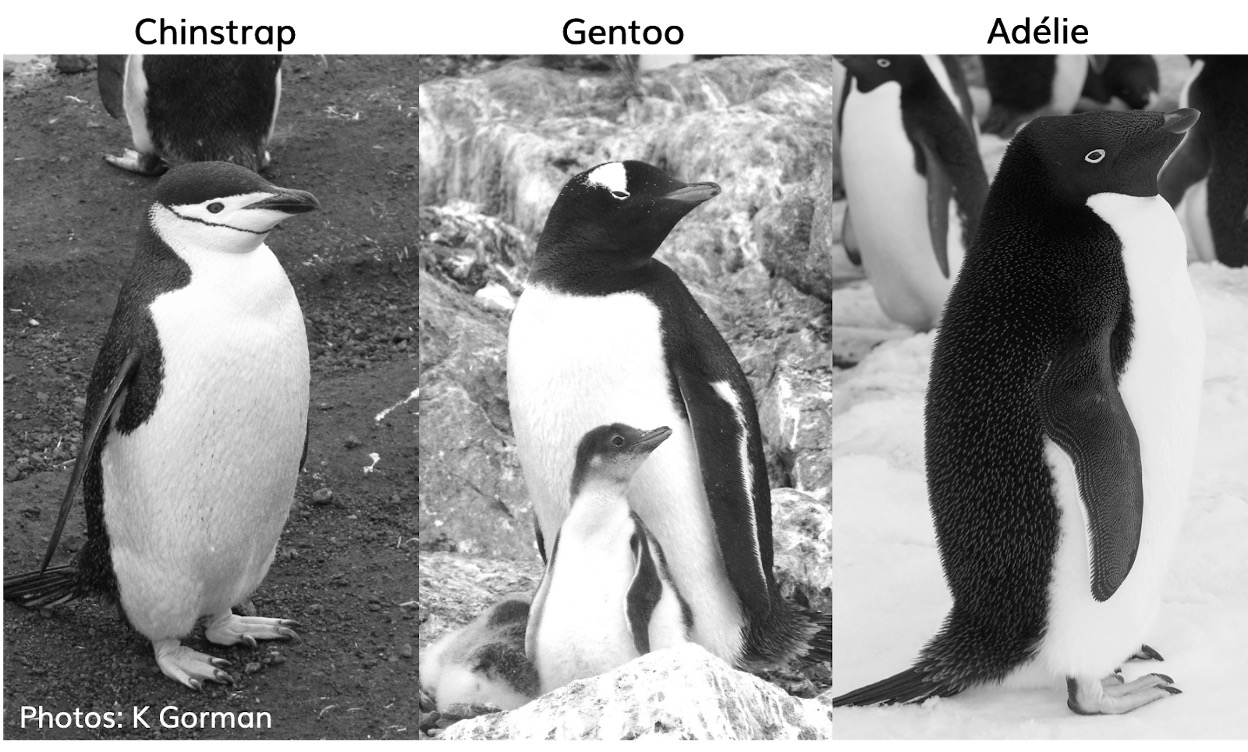
\includegraphics[width=0.8\linewidth]{images/gorman-penguins}

These data were collected from 2007 - 2009 by Dr.~Kristen Gorman with the Palmer Station Long Term Ecological Research Program, part of the US Long Term Ecological Research Network. The data were imported directly from the Environmental Data Initiative (EDI) Data Portal, and are available for use by CC0 license (``No Rights Reserved'') in accordance with the Palmer Station Data Policy. We gratefully acknowledge Palmer Station LTER and the US LTER Network. Special thanks to Marty Downs (Director, LTER Network Office) for help regarding the data license \& use. Here is our intrepid package co-author, Dr.~Gorman, in action collecting some penguin data:

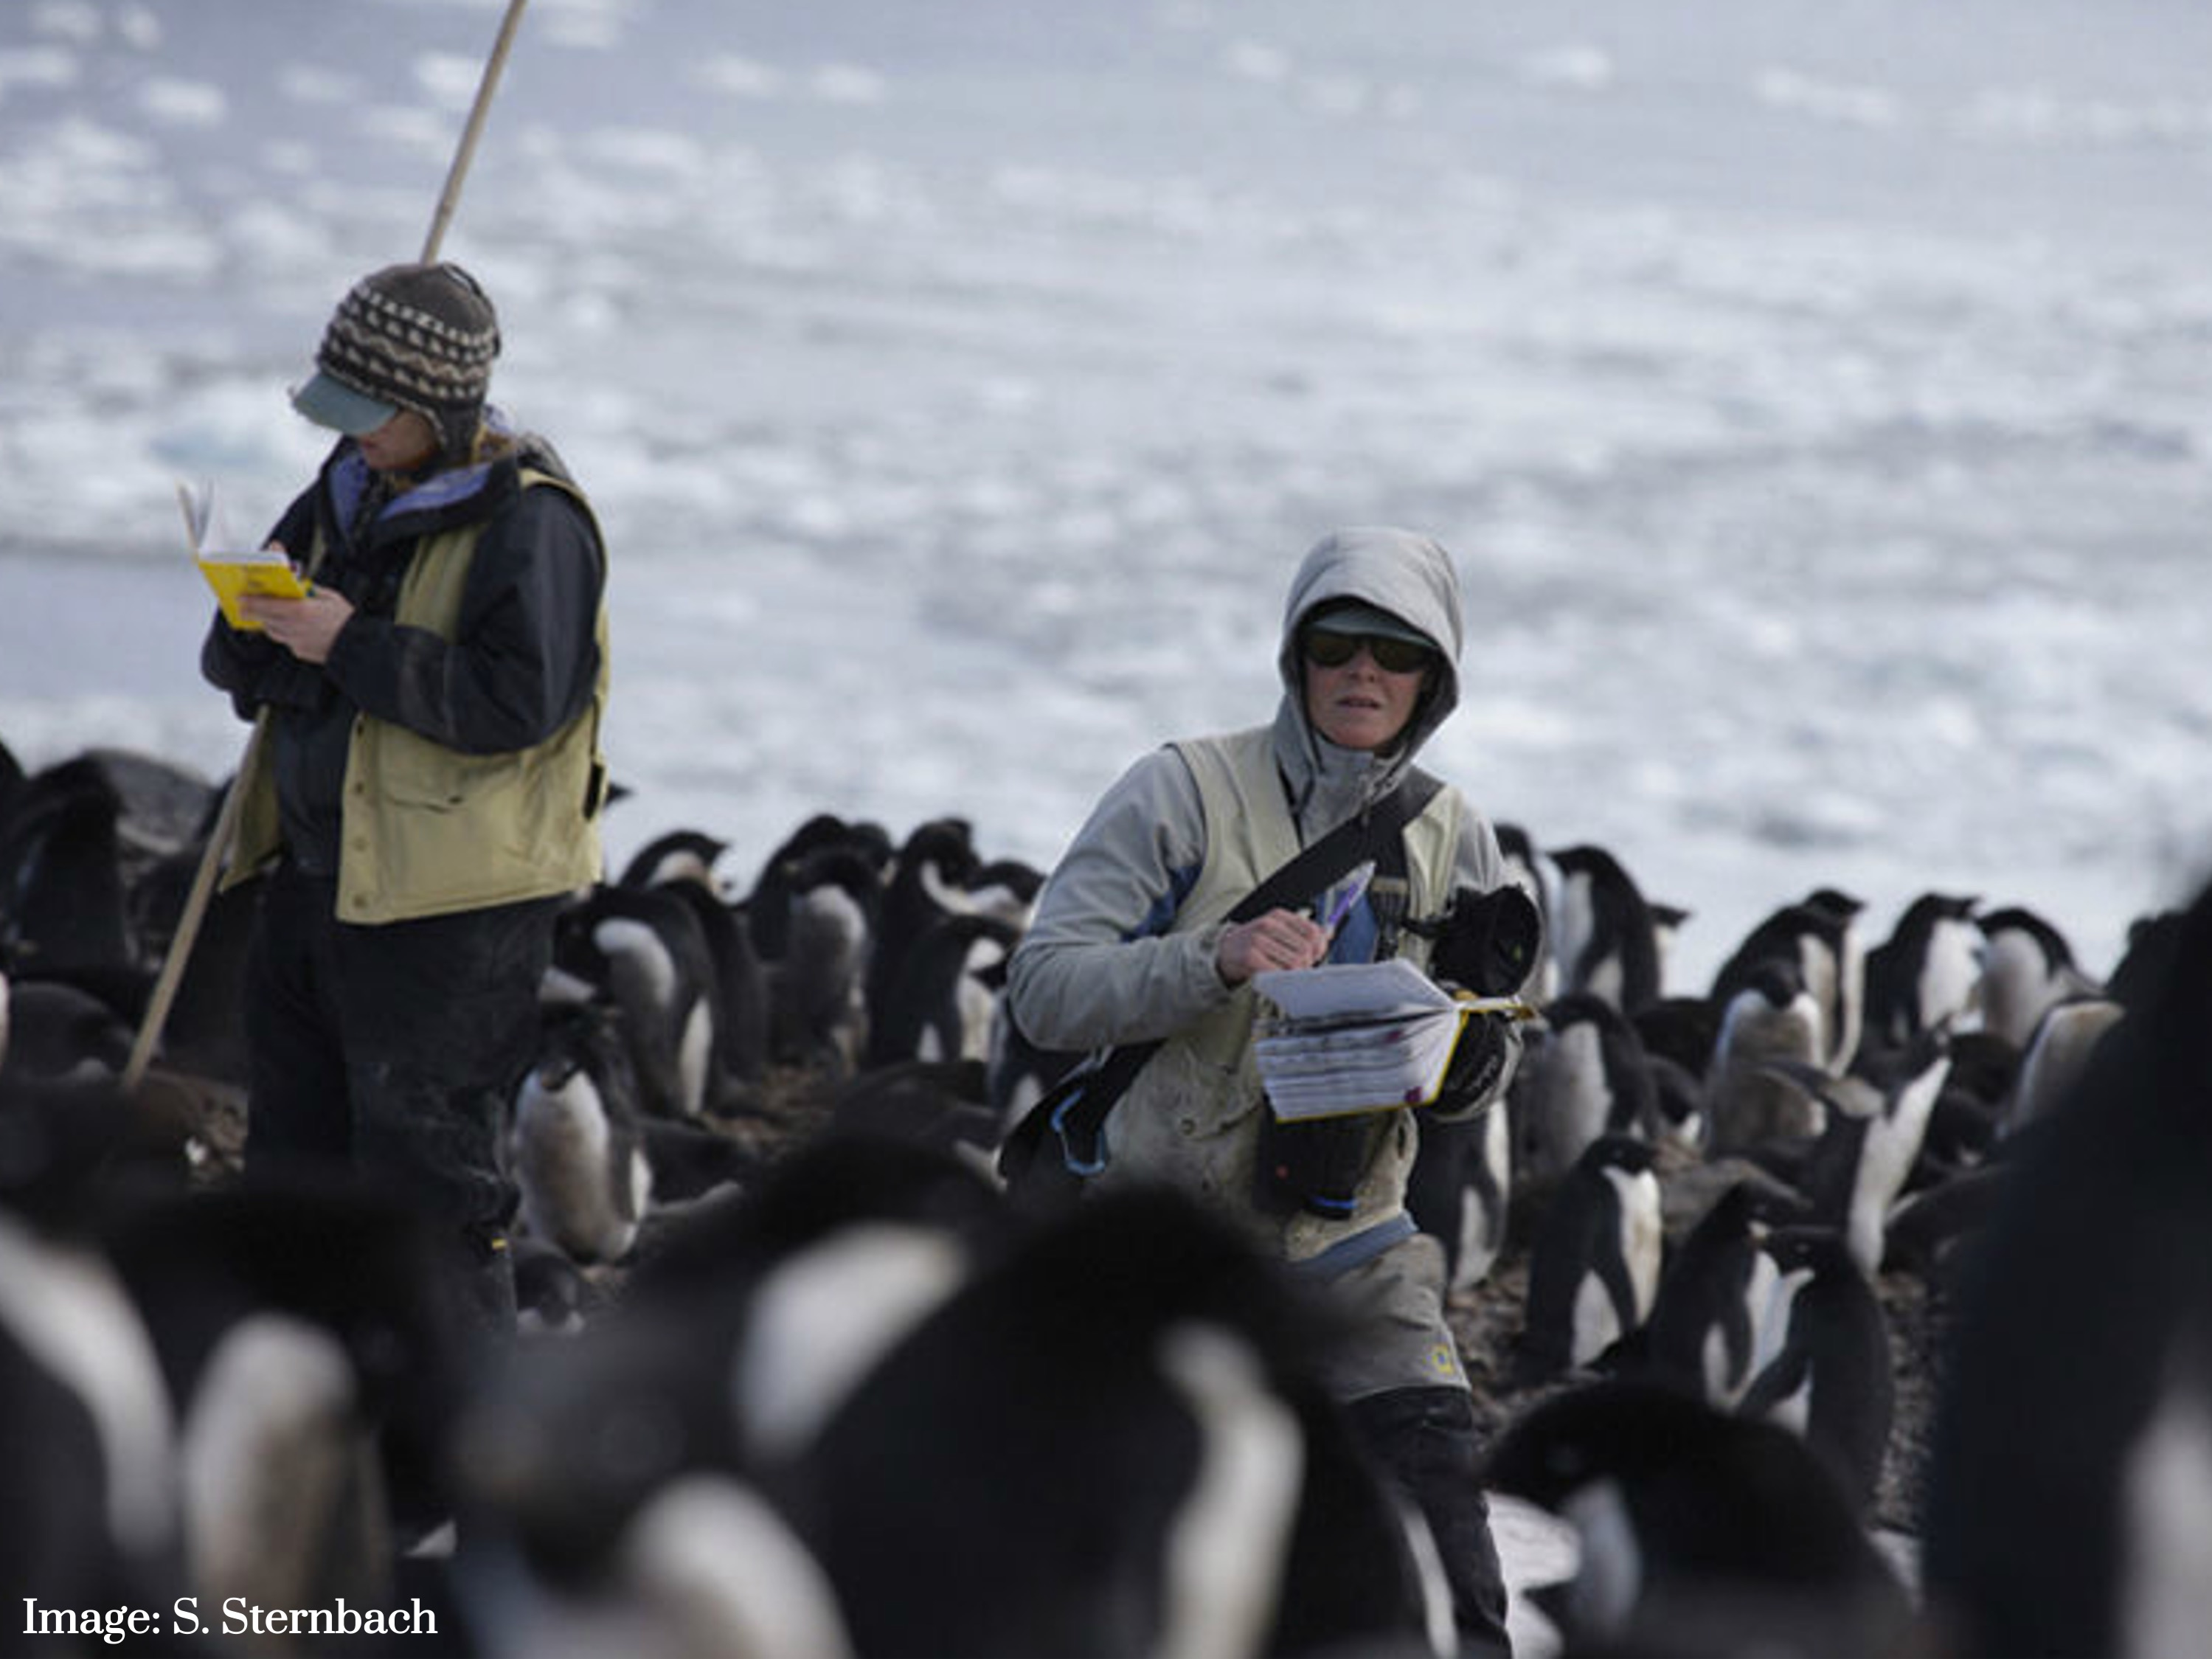
\includegraphics[width=0.8\linewidth]{images/penguin-expedition}

Here is a map of the study site

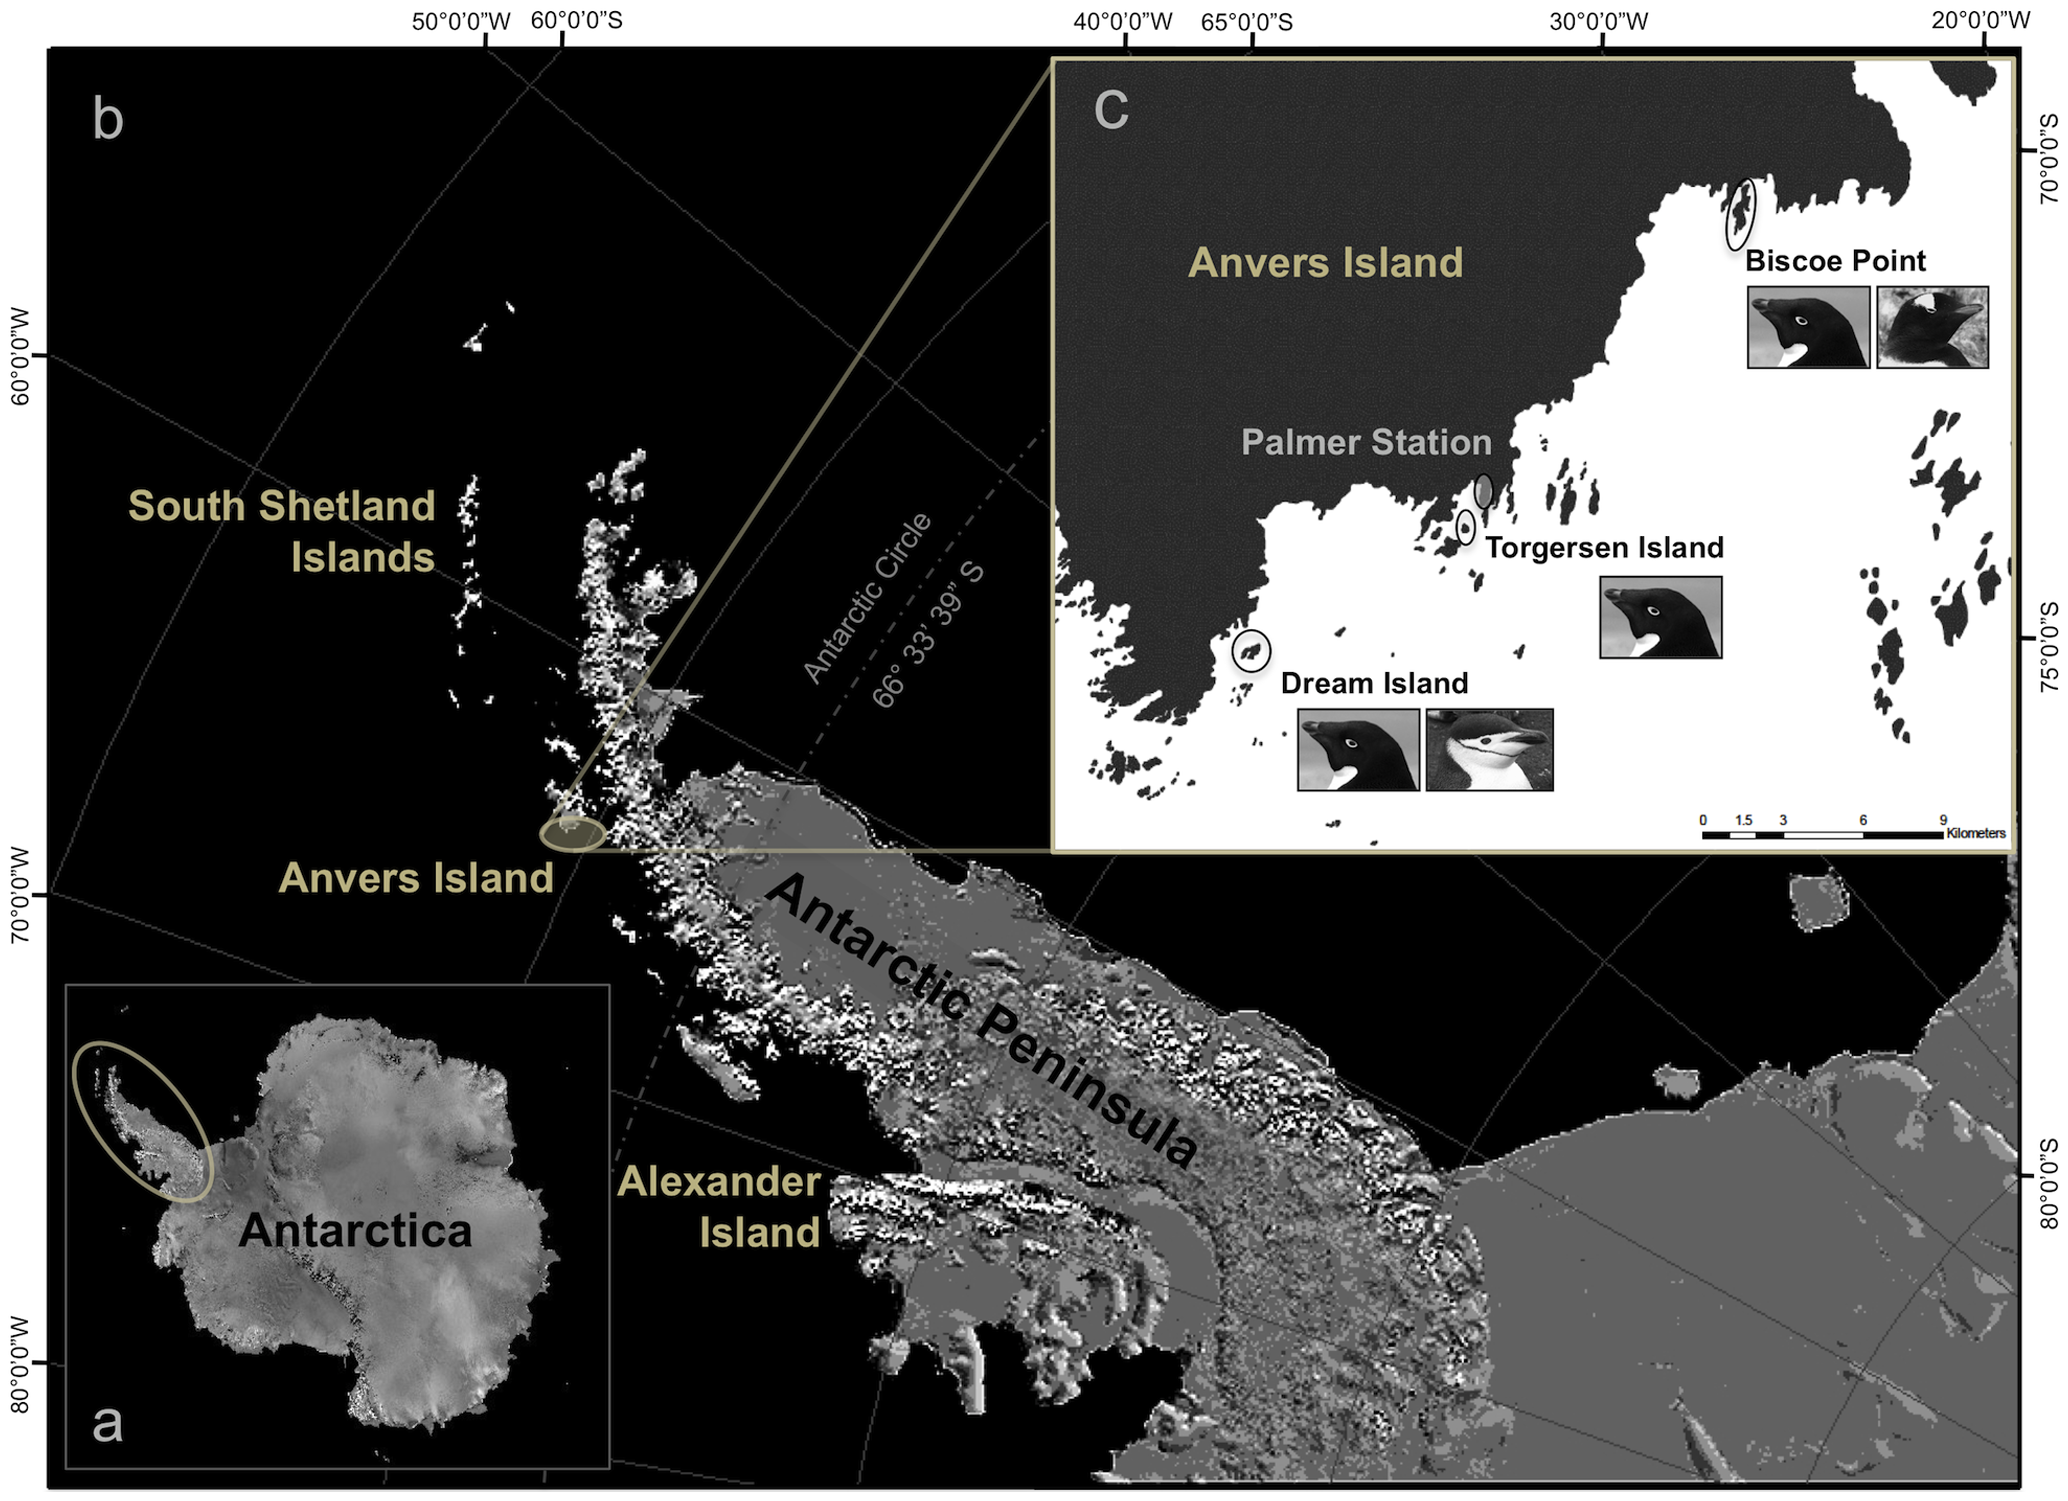
\includegraphics[width=0.8\linewidth]{images/antarctica-map}

\hypertarget{insights-from-data}{%
\subsection{Insights from data}\label{insights-from-data}}

This dataset is relatively simple, as there aren't too many variables to consider. But there are a reasonably large number of datapoints (individual penguins) making it possible to generate insights.

However, there are some specific and rather common problems in this data. Problems that we need to work through \emph{before} we can start to make any visuals or try to draw any conclusions. There are some problems with the variable names, there are some problems with some of the values. There are problems that one of the response variables isn't actually encoded on the dataset (we have to make it).

Today we are going to

\begin{itemize}
\item
  Formulate clear research questions
\item
  Import our dataset
\item
  Learn how to prepare our RStudio Project workspace
\item
  Learn how to clean, tidy and manipulate our data to allow tables, graphs and analyses to be run
\end{itemize}

Don't worry if you don't understand exactly what each function does at the moment, or struggle to remember every concept we are introduced to. We will cover these again, in lots more detail as we progress. The main point is to get familiar with our process for handling data and organising our projects.

\hypertarget{the-question}{%
\section{The Question?}\label{the-question}}

Imagine that you are a Penguin biologist. Chilly.

Imagine that you want to know more about the feeding habits of the different penguin species in the Antarctic. You also wish to characterise features such as bill morphology, and body size and compare them across species. Adelie and Chinstrap penguins are off-shore, shallow diving foragers, while Gentoo's feed closer inshort and are deep-divers. We might expect that we can find some features of Gentoo's that align with their different lifestyle/feeding habits.

With simple measuring techniques and identification skills we can sex the penguins, identify their species and take simple non-invasive measurements of features such as body size, flipper length and bill dimensions. You also recently read a paper about the ratios of different Nitrogen and Carbon isotopes in blood, and how these can be used to infer the types of prey that are forming an organism's diet.

\hypertarget{hypotheses}{%
\subsection{Hypotheses}\label{hypotheses}}

These hypotheses are fairly basic, we have not included directionality or specific expecations of the magnitude of the difference. This would come from doing more research on the subject area.

\begin{itemize}
\item
  The bill lengths/depths ratio to body size of Gentoo penguins will be different to Adelie and Chinstrap penguins.
\item
  Gentoo penguins will have a different N and carbon isotope ratio than Adelie and Chinstrap penguins.
\end{itemize}

\hypertarget{preparing-the-data}{%
\section{Preparing the data}\label{preparing-the-data}}

Imagine we have completed our practical study and have our data. The data is probably distributed in lots of places, originally notes collected in the field were probably on paper \& notebooks. Then someone will have taken time to transcribe those into a spreadsheet. This will almost certainly have been done by typing all the data in by hand.

It is very important for us to know how we would like our data to be organised at the end. We are going to learn how to organise data using the \emph{tidy} format\footnote{(\url{http://vita.had.co.nz/papers/tidy-data.pdf})}. This is because we are going to use the \texttt{tidyverse} packages by \citet{tidyverse2019}. This is an opinionated, but highly effective method for generating reproducible analyses with a wide-range of data manipulation tools. Tidy data is an easy format for computers to read.

\hypertarget{tidy-data}{%
\subsection{Tidy data}\label{tidy-data}}

Here `tidy' refers to a specific structure that lets us manipulate and visualise data with ease. In a tidy dataset each \emph{variable} is in one column and each row contains one \emph{observation}. Each cell of the table/spreadsheet contains the \emph{values}. Obe observation you might make about tidy data is it is quite long - it generates a lot of rows of data.

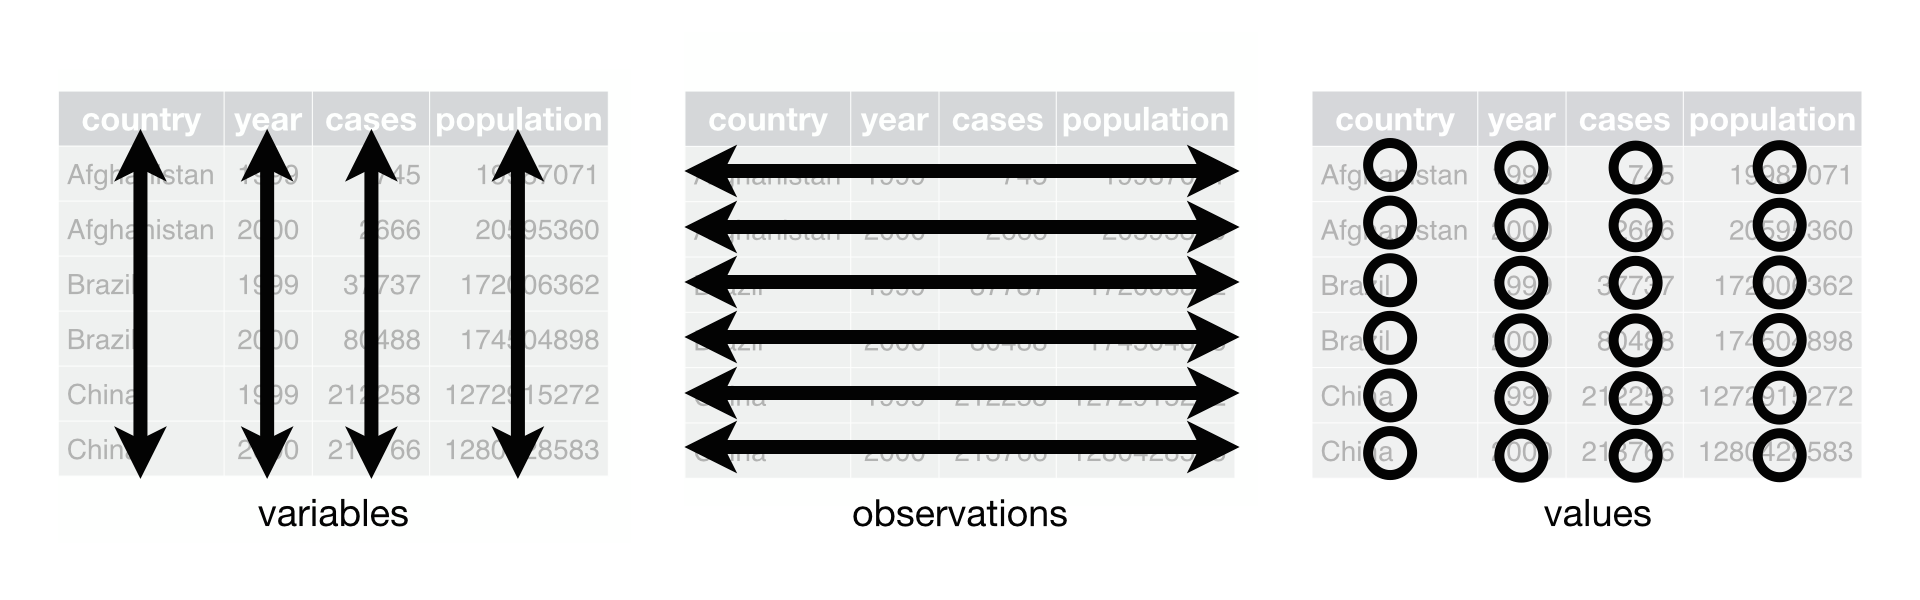
\includegraphics[width=0.8\linewidth]{images/tidy-1}

Typing data in, using any spreadsheet program (e.g.~Excel, Google sheets), if we type in the penguin data, we would make each row contain one observation about one penguin. If we made a second observation about a penguin (say in the next year of the study) it would get a new row in the dataset. You are probably thinking this is a lot of typing and a lot of repetition - and you are right! But this format allows the computer to easily make summaries at any level.

If the data we input to R is ``untidy'' then we have to spend a little bit of time tidying, we will explore this more later.

Once data has been typed up into a spreadsheet and double/triple-checked against the original paper records, then they are saved as a `comma-separated values (CSV)' file-type. These files are the simplest form of database, no coloured cells, no formulae, no text formatting. Each row is a row of the data, each value of a row (previously separate columns) is separated by a comma.

It is convenient to use something like Excel to type in our data - its much more usefully friendly than trying to tpye something in csv format. But we don't save files in the Excel format because they have a nasty habit of formatting or even losing data when the file gets large enough \footnote{\url{https://www.theguardian.com/politics/2020/oct/05/how-excel-may-have-caused-loss-of-16000-covid-tests-in-england}}.
If you need to add data to a csv file, you can always open it in an Excel-like program and add more information.

\begin{figure}
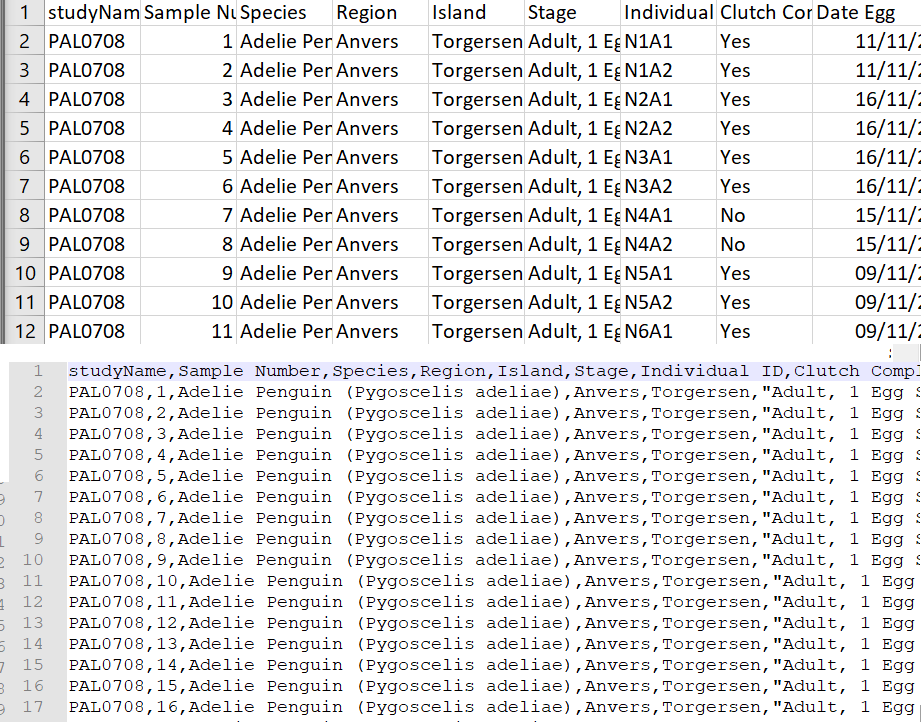
\includegraphics[width=0.8\linewidth]{images/excel_csv} \caption{Top image: Penguins data viewed in Excel, Bottom image: Penguins data in native csv format}\label{fig:unnamed-chunk-45}
\end{figure}

It is possible to import data into R in an Excel format, but I recommend sticking with csv formats. Any spreadsheet can be easily converted with the \emph{Save As..} command.

\hypertarget{the-dataset}{%
\subsection{The dataset}\label{the-dataset}}

For today's workshop we want to acquire the dataset to work on it. We can retrieve the file we need from here (\url{https://github.com/UEABIO/5023Y_Workshop/blob/main/data/penguins_raw.csv}).

\begin{figure}
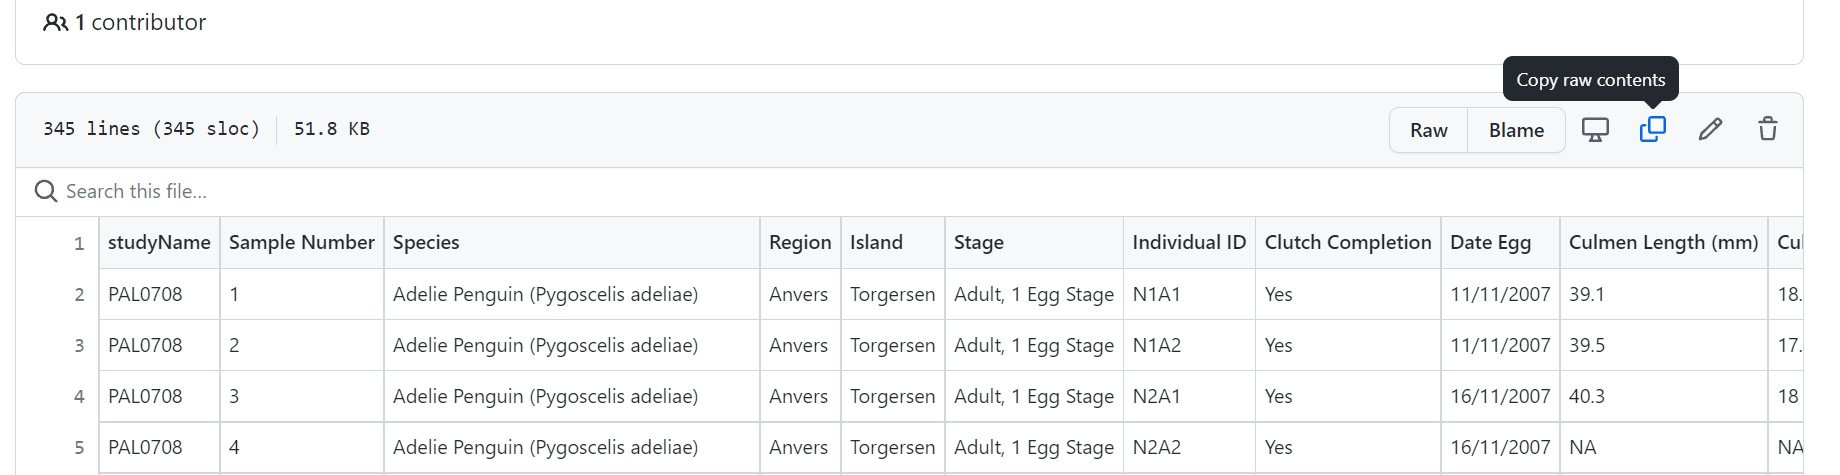
\includegraphics[width=1\linewidth]{images/penguin_github} \caption{Click on the copy raw contents button}\label{fig:unnamed-chunk-46}
\end{figure}

We then need to

\begin{enumerate}
\def\labelenumi{\arabic{enumi}.}
\item
  Select the copy raw contents button
\item
  Open a blank notepad
\item
  Paste the contents
\item
  Save the file as `penguin\_data.csv'
\item
  Open the newly saved file in Excel and take a look
\end{enumerate}

We can see a dataset with 345 rows (including the headers) and 17 variables

\begin{itemize}
\item
  \textbf{Study name}: an identifier for the year in which sets of observations were made
\item
  \textbf{Region}: the area in which the observation was recorded
\item
  \textbf{Island}: the specific island where the observation was recorded
\item
  \textbf{Stage}: Denotes reproductive stage of the penguin
\item
  \textbf{Individual} ID: the unique ID of the individual
\item
  \textbf{Clutch completion}: if the study nest observed with a full clutch e.g.~2 eggs
\item
  \textbf{Date egg}: the date at which the study nest observed with 1 egg
\item
  \textbf{Culmen length}: length of the dorsal ridge of the bird's bill (mm)
\item
  \textbf{Culmen depth}: depth of the dorsal ridge of the bird's bill (mm)
\item
  \textbf{Flipper Length}: length of bird's flipper (mm)
\item
  \textbf{Body Mass}: Bird's mass in (g)
\item
  \textbf{Sex}: Denotes the sex of the bird
\item
  \textbf{Delta 15N} : the ratio of stable Nitrogen isotopes 15N:14N from blood sample
\item
  \textbf{Delta 13C}: the ratio of stable Carbon isotopes 13C:12C from blood sample
\end{itemize}

\hypertarget{prepare-the-rstudio-workspace}{%
\section{Prepare the RStudio workspace}\label{prepare-the-rstudio-workspace}}

Now we should have our question, we understand more about where the data came from, and we have our data in a CSV format.

The next step of our workflow is to have a well organised project space. RStudio Cloud does a lot of the hard work for you, each new data project can be set up with its own Project space.

We will define a project as a series of linked questions that uses one (or sometimes several) datasets. For example a coursework assignment for a particular module would be its own project, or eventually your final year research project.

A Project will contain several files, possibly organised into sub-folders containing data, R scripts and final outputs. You might want to keep any information (wider reading) you have gathered that is relevant to your project.

Open the Week Two - workflow project on RStudio Cloud.

Within this project you will notice there is already one file \emph{.Rproj}. This is an R project file, this is a very useful feature, it interacts with R to tell it you are working in a very specific place on the computer (in this case the cloud server we have dialed into). It means R will automatically treat the location of your project file as the `working directory' and makes importing and exporting easier\footnote{More on projects can be found in the R4DS book (\url{https://r4ds.had.co.nz/workflow-projects.html})}.

\hypertarget{organise}{%
\subsection{Organise}\label{organise}}

Now we are going to organise our workspace, first its always a good first step to go to Tools \textgreater{} Project options and switch all of the options for saving and loading .Rdata to `No'

Then we create the following folders:

\begin{itemize}
\item
  data
\item
  scripts
\item
  figures
\end{itemize}

\begin{rmdwarning}
Make sure you type these \textbf{exactly} as printed here - remember
that to R is case-sensitive so `data' and `Data' are two different
things!
\end{rmdwarning}

Having these separate subfolders within our project helps keep things tidy, means it's harder to lose things, and lets you easily tell R exactly where to go to retrieve data.

Now do you remember where you saved the `penguin\_data.csv' file? I hope so!!! Go to the upload button in the Files tab of RStudio Cloud and tell it where the file is located on your local computer and upload it to the `data' folder you have made in your Project.

\begin{figure}
\includegraphics[width=0.8\linewidth]{images/project} \caption{An example of a typical R project set-up}\label{fig:unnamed-chunk-48}
\end{figure}

\hypertarget{create-a-new-r-script}{%
\subsection{Create a new R script}\label{create-a-new-r-script}}

Let's now create a new R script file in which we will write instructions and store comments for manipulating data, developing tables and figures. Use the File \textgreater{} New Script menu item and select an R Script.

Add the following:

\begin{Shaded}
\begin{Highlighting}[]
\CommentTok{\# An analysis of the bill dimensions of male and female Adelie, Gentoo and Chinstrap penguins. }

\CommentTok{\# Data first published in  Gorman, KB, TD Williams, and WR Fraser. 2014. “Ecological Sexual Dimorphism and Environmental Variability Within a Community of Antarctic Penguins (Genus Pygoscelis).” PLos One 9 (3): e90081. https://doi.org/10.1371/journal.pone.0090081.}
\end{Highlighting}
\end{Shaded}

Then load the following add-on package to the R script, just underneath these comments. Tidyverse isn't actually one package, but a bundle of many different packages that play well together - for example it \emph{includes} \texttt{ggplot2} which we used in the last session, so we don't have to call that separately

\begin{Shaded}
\begin{Highlighting}[]
\FunctionTok{library}\NormalTok{(tidyverse) }\CommentTok{\# tidy data packages}
\FunctionTok{library}\NormalTok{(janitor) }\CommentTok{\# cleaning variable names}
\FunctionTok{library}\NormalTok{(lubridate) }\CommentTok{\# make sure dates are processed properly}
\end{Highlighting}
\end{Shaded}

Now save this file in the scripts folder and call it \emph{penguin\_measurements.R}

\hypertarget{get-the-data-into-r}{%
\section{Get the data into R}\label{get-the-data-into-r}}

Now we are \emph{finally} ready to import the data into R.

Add the following code to your script, then starting at line 1 - ask your script to run in order, library function first as the \texttt{read\_csv()} function is from an add-on package \texttt{readr}

\begin{Shaded}
\begin{Highlighting}[]
\CommentTok{\# read in the data from the data folder in my project}
\NormalTok{penguins }\OtherTok{\textless{}{-}} \FunctionTok{read\_csv}\NormalTok{(}\StringTok{"data/penguins\_data.csv"}\NormalTok{)}
\end{Highlighting}
\end{Shaded}

\begin{verbatim}
Error!
\end{verbatim}

Houston we have a problem! We got an error!!! blah blah does not exist in current working directory

This usually happens if we told R to look in the wrong place, or didn't give it the correct name of what to look for. Can you spot what the mistake was?

Edit your existing line of script to replace it with the proper file name and run the command again.

\begin{Shaded}
\begin{Highlighting}[]
\CommentTok{\# read in the data from the data folder in my project}
\NormalTok{penguins }\OtherTok{\textless{}{-}} \FunctionTok{read\_csv}\NormalTok{(}\StringTok{"data/penguins\_data.csv"}\NormalTok{)}
\end{Highlighting}
\end{Shaded}

\begin{verbatim}
Parsed with column specification:
cols(
  studyName = col_character(),
  `Sample Number` = col_double(),
  Species = col_character(),
  Region = col_character(),
  Island = col_character(),
  Stage = col_character(),
  `Individual ID` = col_character(),
  `Clutch Completion` = col_character(),
  `Date Egg` = col_character(),
  `Culmen Length (mm)` = col_double(),
  `Culmen Depth (mm)` = col_double(),
  `Flipper Length (mm)` = col_double(),
  `Body Mass (g)` = col_character(),
  Sex = col_character(),
  `Delta 15 N (o/oo)` = col_double(),
  `Delta 13 C (o/oo)` = col_double(),
  Comments = col_character()
)
\end{verbatim}

Great, no error this time, the \texttt{read\_csv()} function has read the data and we \textless- assigned this data to the object \texttt{penguins}. If you look in the environment pane you should see the object \texttt{penguins}.

The lines printed in the R console tell us the names of the columns that were identified in the file and the type of variable R thinks it is

\begin{itemize}
\item
  \texttt{col\_character()} means the column contains letters or words
\item
  \texttt{col\_double()} means the column contains numbers
\end{itemize}

\begin{rmdquestion}
Have a look - do all of these seem correct to you? If not we should fix
these, and we will get onto that in a little bit.
\end{rmdquestion}

\hypertarget{view-and-refine}{%
\subsection{View and refine}\label{view-and-refine}}

So we know our data is in R, and we know the columns and names have been imported. But we still don't know whether all of our values imported, or whether it captured all the rows.

There are lots of different ways to view and check data. One useful method is \texttt{glimpse}

\begin{Shaded}
\begin{Highlighting}[]
\CommentTok{\# check the structure of the data}
\FunctionTok{glimpse}\NormalTok{(penguins)}
\end{Highlighting}
\end{Shaded}

When we run \texttt{glimpse()} we get several lines of output. The number of observations ``rows'', the number of variables ``columns''. Check this against the csv file you have - they should be the same. In the next lines we see variable names and the type of data.

We should be able to see by now, that all is not well!!! \texttt{Body\ Mass\ (g)} is being treated as character (string), as is \texttt{Date\ Egg}, meaning R thinks these contain letters and words instead of numbers and dates.

Other ways to view the data

\begin{itemize}
\item
  type \texttt{penguins} into the Console
\item
  type \texttt{view(penguins)} this will open a spreadsheet in a new tab
\item
  type \texttt{head(penguins)} will show the first 10 lines of the data, rather than the whole dataset
\end{itemize}

\begin{quote}
**Note - \texttt{view()} lets you do cool stuff like reorder rows and quickly scroll through the dataset without affecting the underlying data.
\end{quote}

\hypertarget{data-management}{%
\subsection{Data management}\label{data-management}}

We've imported the data, checked it and found some inconsistencies.

This is where we start to use some of the core functions from \texttt{tidyverse}.

If R thinks \texttt{Body\ Mass\ (g)} is a character variable, then it probably contains some words as well as numbers. So let's have a look at this and compare it to a variable which has been processed correctly

\begin{Shaded}
\begin{Highlighting}[]
\CommentTok{\# get the first 10 rows of the Flipper Length and Body Mass variables}
\NormalTok{penguins }\SpecialCharTok{\%\textgreater{}\%} 
  \FunctionTok{select}\NormalTok{(}\StringTok{\textasciigrave{}}\AttributeTok{Flipper Length (mm)}\StringTok{\textasciigrave{}}\NormalTok{, }
         \StringTok{\textasciigrave{}}\AttributeTok{Body Mass (g)}\StringTok{\textasciigrave{}}\NormalTok{) }\SpecialCharTok{\%\textgreater{}\%} 
  \FunctionTok{head}\NormalTok{(}\DecValTok{10}\NormalTok{) }\CommentTok{\# 10 rows}
\end{Highlighting}
\end{Shaded}

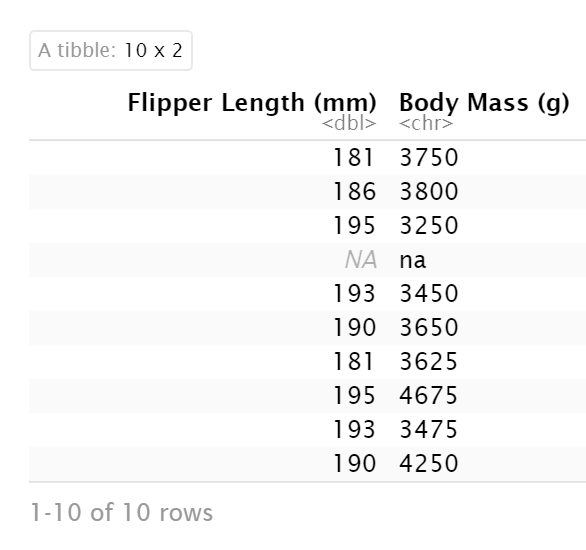
\includegraphics[width=0.8\linewidth]{images/NA}

\begin{quote}
**Note - What is the \%\textgreater\% ??? It's known as a pipe. It sends the results of one line of code to the next. So the data penguins is sent to the \texttt{select} function which picks only those variables we want. The result of this is then sent to the \texttt{head} function which with the argument for number of rows set to 10, prints the top 10 rows.
\end{quote}

\begin{quote}
The other way to write this series of functions would be to use brackets and the rules of BODMAS:
\end{quote}

\begin{verbatim}
head(select(penguins, `Flipper Length (mm)`, `Body Mass (g)`),10)
\end{verbatim}

\begin{quote}
Hopefully you agree that the pipes make the code a lot more human-reader friendly. More on pipes later
\end{quote}

So what's the problem with our data? in the Flipper length variable, missing observations have been correctly marked as \texttt{NA} signifying missing data. R can handle missing data just fine. However, in thew Body mass variable, it looks as though someone has actually typed ``na'' in observations where the data is missing. Here R has failed to recognise an \texttt{NA} and has read it as a word instead. This is because \texttt{read\_csv()} looks for gaps or \texttt{NA} but not ``na''.

No problem this is an easy fix. Head back to your script and make the following edit the line for data importing

\begin{Shaded}
\begin{Highlighting}[]
\CommentTok{\# read in the penguins data, specify that NA strings can be "na" or "NA"}
\NormalTok{penguins }\OtherTok{\textless{}{-}} \FunctionTok{read\_csv}\NormalTok{(}\StringTok{"data/penguin\_data.csv"}\NormalTok{, }\AttributeTok{na=}\FunctionTok{c}\NormalTok{(}\StringTok{"na"}\NormalTok{,}\StringTok{"NA"}\NormalTok{))}
\end{Highlighting}
\end{Shaded}

Now re-check your data using the same lines of code from before.
All ok now?

\hypertarget{dataframes-and-tibbles}{%
\section{Dataframes and tibbles}\label{dataframes-and-tibbles}}

A quick sidebar on how R stores data. When we imported the data into R it ws put into an object called a \textbf{tibble} which is a type of \textbf{dataframe}.

Let's have a quick go at making our own \textbf{tibble} from scratch.

Make a new script called `TibbleTrouble.R' in the scripts folder as before.

At the top of this new script put

\begin{Shaded}
\begin{Highlighting}[]
\CommentTok{\# just me messing about making tibbles}

\CommentTok{\# libraries}
\FunctionTok{library}\NormalTok{(tidyverse)}

\CommentTok{\# make some variables, when we have a one dimensional object like this it is known as an atomic vector!}
\NormalTok{person }\OtherTok{\textless{}{-}} \FunctionTok{c}\NormalTok{(}\StringTok{"Mark"}\NormalTok{, }\StringTok{"Phil"}\NormalTok{, }\StringTok{"Becky"}\NormalTok{, }\StringTok{"Tony"}\NormalTok{)}
\NormalTok{hobby }\OtherTok{\textless{}{-}} \FunctionTok{c}\NormalTok{(}\StringTok{"kickboxing"}\NormalTok{, }\StringTok{"coding"}\NormalTok{, }\StringTok{"dog walking"}\NormalTok{, }\StringTok{"car boot sales"}\NormalTok{)}
\NormalTok{awesomeness }\OtherTok{\textless{}{-}} \FunctionTok{c}\NormalTok{(}\DecValTok{1}\NormalTok{,}\DecValTok{100}\NormalTok{,}\DecValTok{1}\NormalTok{,}\DecValTok{1}\NormalTok{)}
\end{Highlighting}
\end{Shaded}

The function \texttt{c} lets you `concatenate' or link each of these arguments together into a single vector.

Now we put these vectors together, where they become the variables in a new tibble

\begin{Shaded}
\begin{Highlighting}[]
\CommentTok{\# make a tibble}
\NormalTok{my\_data }\OtherTok{\textless{}{-}} \FunctionTok{tibble}\NormalTok{(person, hobby, awesomeness)}
\NormalTok{my\_data}
\end{Highlighting}
\end{Shaded}

\begin{verbatim}
# A tibble: 4 x 3
  person hobby          awesomeness
  <chr>  <chr>                <dbl>
1 Mark   kickboxing               1
2 Phil   coding                 100
3 Becky  dog walking              1
4 Tony   car boot sales           1
\end{verbatim}

Have a go at messing about with your script and figure out what each of these does, add comments and save your script.

\begin{Shaded}
\begin{Highlighting}[]
\CommentTok{\# Some R functions for looking at tibbles and dataframes I will comment next to each one with what it does}

\FunctionTok{head}\NormalTok{(my\_data, }\AttributeTok{n=}\DecValTok{2}\NormalTok{)}
\FunctionTok{tail}\NormalTok{(my\_data, }\AttributeTok{n=}\DecValTok{1}\NormalTok{)}
\FunctionTok{nrow}\NormalTok{(my\_data)}
\FunctionTok{ncol}\NormalTok{(my\_data)}
\FunctionTok{colnames}\NormalTok{(my\_data)}
\FunctionTok{view}\NormalTok{(my\_data)}
\FunctionTok{glimpse}\NormalTok{(my\_data)}
\FunctionTok{str}\NormalTok{(my\_data)}
\end{Highlighting}
\end{Shaded}

\hypertarget{clean-and-tidy}{%
\section{Clean and tidy}\label{clean-and-tidy}}

Back to your penguins script.

We have checked the data imported correctly, now its time to \emph{clean and tidy} the data.

\hypertarget{tidy}{%
\subsection{Tidy}\label{tidy}}

In this example our data is already in \texttt{tidy} format i.e.~one observation per row. We will cover what to do if data isn't tidy later.

\hypertarget{clean}{%
\subsection{Clean}\label{clean}}

Here are a few things we might want to do to our data to make it `clean'.

\begin{itemize}
\item
  Refine variable names
\item
  Format dates and times
\item
  Rename some values
\item
  Check for any duplicate records
\item
  Check for any implausible data or typos
\item
  Check and deal with missing values
\end{itemize}

\begin{quote}
**Note - Remember because we are doing everything in a script, the original data remains unchanged. This means we have data integrity, and a clear record of what we did to tidy and clean a dataset in order to produce summaries and data visuals
\end{quote}

\hypertarget{refine-variable-names}{%
\subsection{Refine variable names}\label{refine-variable-names}}

Often we might want to change the names of our variables. They might be non-intuitive, or too long. Our data has a couple of issues:

\begin{itemize}
\item
  Some of the names contain spaces
\item
  Some of the names contain brackets
\end{itemize}

Let's correct these quickly

\begin{Shaded}
\begin{Highlighting}[]
\CommentTok{\#clean all variable names to snake\_case using the clean\_names function from the janitor package}
\CommentTok{\# note we are using assign \textless{}{-} to overwrite the old version of penguins with a version that has updated names}
\CommentTok{\# this changes the data in our R workspace but not the original csv file}

\NormalTok{penguins }\OtherTok{\textless{}{-}}\NormalTok{ penguins }\SpecialCharTok{\%\textgreater{}\%} \CommentTok{\#}
\NormalTok{  janitor}\SpecialCharTok{::}\FunctionTok{clean\_names}\NormalTok{()}

\FunctionTok{colnames}\NormalTok{(penguins) }\CommentTok{\# quickly check the new variable names}
\end{Highlighting}
\end{Shaded}

\begin{quote}
**Note - in this example you can see that I put the name of the package janitor, in front of the function \texttt{clean\_names}. But if I have already loaded the package with library(janitor) then this isn't strictly necessary and penguins \%\textgreater\% clean\_names() would also have worked just fine. So why do this? Remember when we loaded the tidyverse package - we got a warning about conflicts - this was because two of our packages \texttt{dplyr} and \texttt{stats} have functions that are different, but share the same name. But we can make sure we call the one we want by specifying which package we are calling a function from. We don't need to do this very often, but it's good to know.
\end{quote}

\begin{verbatim}
> library(tidyverse)
-- Attaching packages --------------------------------------- tidyverse 1.3.0 --
v ggplot2 3.3.2     v purrr   0.3.4
v tibble  3.0.4     v dplyr   1.0.2
v tidyr   1.1.2     v stringr 1.4.0
v readr   1.3.1     v forcats 0.5.0
-- Conflicts ------------------------------------------ tidyverse_conflicts() --
x dplyr::filter() masks stats::filter()
x dplyr::lag()    masks stats::lag()
\end{verbatim}

The \texttt{clean\_names} function quickly converts all variable names into snake case. The N and C blood isotope ratio names are still quite long though, so let's clean those with \texttt{dplyr::rename()} where ``new\_name'' = ``old\_name''.

\begin{Shaded}
\begin{Highlighting}[]
\CommentTok{\# shorten the variable names for N and C isotope blood samples}

\NormalTok{penguins }\OtherTok{\textless{}{-}}\NormalTok{ penguins }\SpecialCharTok{\%\textgreater{}\%} 
  \FunctionTok{rename}\NormalTok{(}\StringTok{"delta\_15n"}\OtherTok{=}\StringTok{"delta\_15\_n\_o\_oo"}\NormalTok{,  }\CommentTok{\# use rename from the dplyr package}
         \StringTok{"delta\_13c"}\OtherTok{=}\StringTok{"delat\_13\_c\_o\_oo"}\NormalTok{)}
\end{Highlighting}
\end{Shaded}

\hypertarget{dates}{%
\subsection{Dates}\label{dates}}

We can also see there is a \texttt{date\_egg} variable. If you check it (using any of the new functions you have learned), you should see that it all looks like its been inputted correctly, but R is treating it as words, rather than assigning it a date value. We can fix that with the \texttt{lubridate} package. If we use the function \texttt{dmy} then we tell R this is date data in date/month/year format.

\begin{Shaded}
\begin{Highlighting}[]
\CommentTok{\# use dmy from stringr package to encode date properly}
\NormalTok{penguins }\OtherTok{\textless{}{-}}\NormalTok{ penguins }\SpecialCharTok{\%\textgreater{}\%} 
  \FunctionTok{mutate}\NormalTok{(}\AttributeTok{date\_egg\_proper=}\FunctionTok{dmy}\NormalTok{(date\_egg))}
\end{Highlighting}
\end{Shaded}

\begin{rmdquestion}
What is the deliberate mistake in my code comment above? By now you may
have picked up there are the odd mistakes (possibly some non-deliberate
ones) - to make sure you aren't just copy-pasting on autpilot.
\end{rmdquestion}

Here we use the \texttt{mutate} function from \texttt{dplyr} to create a new variable called \texttt{date\_egg\_proper} based on the output of converting the characters in \texttt{date\_egg} to date format. The original variable is left intact, if we had specified the ``new'' variable was also called \texttt{date\_egg} then it would have overwritten the original variable.

\hypertarget{rename-some-values}{%
\subsection{Rename some values}\label{rename-some-values}}

Sometimes we may want to rename the values in our variables in order to make a shorthand that is easier to follow.

\begin{Shaded}
\begin{Highlighting}[]
\CommentTok{\# use mutate and case\_when for an if{-}else statement that changes the names of the values in a variable}
\NormalTok{penguins }\OtherTok{\textless{}{-}}\NormalTok{ penguins }\SpecialCharTok{\%\textgreater{}\%} 
  \FunctionTok{mutate}\NormalTok{(}\AttributeTok{species =} \FunctionTok{case\_when}\NormalTok{(species }\SpecialCharTok{==} \StringTok{"Adelie Penguin (Pygoscelis adeliae)"} \SpecialCharTok{\textasciitilde{}} \StringTok{"Adelie"}\NormalTok{,}
\NormalTok{                             species }\SpecialCharTok{==} \StringTok{"Gentoo penguin (Pygoscelis papua)"} \SpecialCharTok{\textasciitilde{}} \StringTok{"Gentoo"}\NormalTok{,}
\NormalTok{                             species }\SpecialCharTok{==} \StringTok{"Chinstrap penguin (Pygoscelis antarctica)"} \SpecialCharTok{\textasciitilde{}} \StringTok{"Chinstrap"}\NormalTok{))}
\end{Highlighting}
\end{Shaded}

\hypertarget{check-for-duplication}{%
\subsection{Check for duplication}\label{check-for-duplication}}

It is very easy when inputting data to make mistakes, copy something in twice for example, or if someone did a lot of copy-pasting to assemble a spreadsheet (yikes!). We can check this pretty quickly

\begin{Shaded}
\begin{Highlighting}[]
\CommentTok{\# check for duplicate rows in the data}
\NormalTok{penguins }\SpecialCharTok{\%\textgreater{}\%} 
  \FunctionTok{duplicated}\NormalTok{() }\SpecialCharTok{\%\textgreater{}\%} \CommentTok{\# produces a list of TRUE/FALSE statements for duplicated or not}
  \FunctionTok{sum}\NormalTok{() }\CommentTok{\# sums all the TRUE statements}
\end{Highlighting}
\end{Shaded}

\begin{verbatim}
[1] 0
\end{verbatim}

Great!

\hypertarget{check-for-typos-or-implausible-values}{%
\subsection{Check for typos or implausible values}\label{check-for-typos-or-implausible-values}}

We can also explore our data for very obvious typos by checking for implausibly small or large values

\begin{Shaded}
\begin{Highlighting}[]
\CommentTok{\# use summarise to make calculations}
\NormalTok{penguins }\SpecialCharTok{\%\textgreater{}\%} 
  \FunctionTok{summarise}\NormalTok{(}\AttributeTok{min=}\FunctionTok{min}\NormalTok{(body\_mass\_g, }\AttributeTok{na.rm=}\ConstantTok{TRUE}\NormalTok{), }
            \AttributeTok{max=}\FunctionTok{max}\NormalTok{(body\_mass\_g, }\AttributeTok{na.rm=}\ConstantTok{TRUE}\NormalTok{))}
\end{Highlighting}
\end{Shaded}

The minimum weight for our penguins is 2.7kg, and the max is 6.3kg - not outrageous. If the min had come out at 27g we might have been suspicious. We will use \texttt{summarise} again to calculate other metrics in the future.

\begin{quote}
**Note - our first data insight, the difference the smallest adult penguin in our dataset is nearly half the size of the largest penguin.
\end{quote}

We can also look for typos by asking R to produce all of the distinct values in a variable. This is more useful for categorical data, where we expect there to be only a few distinct categories

\begin{Shaded}
\begin{Highlighting}[]
\NormalTok{penguins }\SpecialCharTok{\%\textgreater{}\%} 
  \FunctionTok{distinct}\NormalTok{(sex)}
\end{Highlighting}
\end{Shaded}

Here if someone had mistyped e.g.~`FMALE' it would be obvious. We could do the same thing (and probably should have before we changed the names) for species.

\hypertarget{missing-values---na}{%
\subsection{Missing values - NA}\label{missing-values---na}}

There are multiple ways to check for missing values in our data

\begin{Shaded}
\begin{Highlighting}[]
\CommentTok{\# Get a sum of how many observations are missing in our dataframe}
\NormalTok{penguins }\SpecialCharTok{\%\textgreater{}\%} 
  \FunctionTok{is.na}\NormalTok{() }\SpecialCharTok{\%\textgreater{}\%} 
  \FunctionTok{sum}\NormalTok{()}
\end{Highlighting}
\end{Shaded}

But this doesn't tell us where these are, fortunately the function \texttt{summary} does this easily

\begin{Shaded}
\begin{Highlighting}[]
\CommentTok{\# produce a summary of our data}
\FunctionTok{summary}\NormalTok{(penguins)}
\end{Highlighting}
\end{Shaded}

This provides a quick breakdown of the max and min for all numeric variables, as well as a list of how many missing observations there are for each one. As we can see there appear to be two missing observations for measurements in body mass, bill lengths, flipper lengths and several more for blood measures. We don't know for sure without inspecting our data further, \emph{but} it is likely that the two birds are missing multiple measurements, and that several more were measured but didn't have their blood drawn.

We will leave the NA's alone for now, but it's useful to know how many we have.

We've now got a clean \& tidy dataset!!

\hypertarget{summing-up}{%
\section{Summing up}\label{summing-up}}

\hypertarget{what-we-learned}{%
\subsection{What we learned}\label{what-we-learned}}

There was a lot of preparation here, and we haven't really got close to make any major insights. But you have:

\begin{itemize}
\item
  Organised your project space
\item
  Dealt with file formats
\item
  Put data into a specific location and imported into R
\item
  Checked the data import
\item
  Cleaned and tidied the data
\end{itemize}

You have also been introduced to the \texttt{tidyverse} and two of its packages

\begin{itemize}
\item
  \texttt{readr} \citet{R-readr}
\item
  \texttt{dplyr} \citet{R-dplyr}
\end{itemize}

As well as:

\begin{itemize}
\item
  \texttt{janitor} \citet{R-janitor}
\item
  \texttt{lubridate} \citet{R-lubridate}
\end{itemize}

\hypertarget{quitting-1}{%
\subsection{Quitting}\label{quitting-1}}

\begin{rmdwarning}
Remember to \textbf{save} your RScript before you leave. And ideally
don't save your .Rdata!
\end{rmdwarning}

\begin{itemize}
\item
  Close your RStudio Cloud Browser
\item
  Go to Blackboard to complete this week's quiz!
\end{itemize}

\hypertarget{workflow-part-two---week-three}{%
\chapter{Workflow Part Two - Week Three}\label{workflow-part-two---week-three}}

Last week we worked through the journey of importing and tidying data to produce a clean dataset.

It's important to remember what questions you have about the data collected, and to make an outline about what you want to do.

\begin{rmdquestion}
Now is a good time to think about what figures might we want to produce
from our data?

We are mostly interested in observable `differences' between our three
penguin species. What sort of figures might illustrate that?

Sometimes it's good to get a pen/pencil and paper - and sketch the
figure you might want to make.
\end{rmdquestion}

\hypertarget{initial-insights}{%
\section{Initial insights}\label{initial-insights}}

Let's start with some basic insights, perhaps by focusing on further questions about specific variables.

\begin{itemize}
\item
  How many penguins were observed?
\item
  How many Adelie, Gentoo and Chinstrap penguins
\item
  What is the distribution of morphologies such as bill length, body size, flipper length
\end{itemize}

Some of these are very simple in that they are summaries of single variables. Some are more complex, like evaluating the numbers of males and females which are the two groups in the sex variable.

These are `safety-checking' insights. You might already know the answers to some of these questions because you may have been responsible for collecting the data. Checking your answers against what you expect is a good way to check your data has been cleaned properly.

\hypertarget{numbers-and-sex-of-the-penguins}{%
\section{Numbers and sex of the penguins}\label{numbers-and-sex-of-the-penguins}}

\begin{Shaded}
\begin{Highlighting}[]
\CommentTok{\# how many observations of penguins were made}

\NormalTok{penguins }\SpecialCharTok{\%\textgreater{}\%} 
  \FunctionTok{summarise}\NormalTok{(}\FunctionTok{n}\NormalTok{())}

\CommentTok{\# but there are multiple observations of penguins across different years}
\CommentTok{\# n\_distinct deals with this}

\NormalTok{penguins }\SpecialCharTok{\%\textgreater{}\%} 
  \FunctionTok{summarise}\NormalTok{(}\FunctionTok{n\_distinct}\NormalTok{(individual\_id))}
\end{Highlighting}
\end{Shaded}

The answer we get is that there are 190 different penguins observed across our multi-year study.

This answer is provided in a tibble, but the variable name is an ugly composition of the functions applied, but we can modify the code

\begin{Shaded}
\begin{Highlighting}[]
\NormalTok{penguins }\SpecialCharTok{\%\textgreater{}\%} 
  \FunctionTok{summarise}\NormalTok{(}\AttributeTok{num\_penguin\_id=}\FunctionTok{n\_distinct}\NormalTok{(individual\_id))}
\end{Highlighting}
\end{Shaded}

How about the number of penguins observed from each species?

\begin{Shaded}
\begin{Highlighting}[]
\NormalTok{penguins }\SpecialCharTok{\%\textgreater{}\%} 
  \FunctionTok{group\_by}\NormalTok{(species) }\SpecialCharTok{\%\textgreater{}\%} \CommentTok{\# ask for distinct counts in each species}
  \FunctionTok{summarise}\NormalTok{(}\AttributeTok{num\_penguin\_id=}\FunctionTok{n\_distinct}\NormalTok{(individual\_id))}
\end{Highlighting}
\end{Shaded}

By adding the \texttt{group\_by} function we tell R to apply any subsequent functions separately according to the group specified. Let's do this again for male and female penguins

\begin{Shaded}
\begin{Highlighting}[]
\NormalTok{penguins }\SpecialCharTok{\%\textgreater{}\%} 
  \FunctionTok{group\_by}\NormalTok{(sex) }\SpecialCharTok{\%\textgreater{}\%} \CommentTok{\# ask for distinct counts in each species}
  \FunctionTok{summarise}\NormalTok{(}\AttributeTok{num\_penguin\_id=}\FunctionTok{n\_distinct}\NormalTok{(individual\_id))}
\end{Highlighting}
\end{Shaded}

Now what about the number of female Gentoo penguins?

\begin{Shaded}
\begin{Highlighting}[]
\NormalTok{penguins }\SpecialCharTok{\%\textgreater{}\%} 
  \FunctionTok{group\_by}\NormalTok{(sex, species) }\SpecialCharTok{\%\textgreater{}\%} \CommentTok{\# ask for distinct counts in each species}
  \FunctionTok{summarise}\NormalTok{(}\AttributeTok{num\_penguin\_id=}\FunctionTok{n\_distinct}\NormalTok{(individual\_id))}
\end{Highlighting}
\end{Shaded}

Now we have a table that shows each combination of penguin species by sex, we can see for example that 65 unique Male Adelie penguins were observed in our study. We can also see that for 6 Adelie and 5 Gentoo penguins, sex was not recorded.

\begin{quote}
**Note - You have just had a crash course in using the \texttt{pipe} and \texttt{dplyr} to produce quick data summaries. Have a go at making some other summaries of your data, perhaps the numbers of penguins by island or region. Try some combinations.
\end{quote}

\hypertarget{making-a-simple-figure}{%
\subsection{Making a simple figure}\label{making-a-simple-figure}}

Let's translate some of our simple summaries into graphs.

\begin{Shaded}
\begin{Highlighting}[]
\CommentTok{\# make summary data and assign to an object with a sensible name we can use}
\NormalTok{penguin\_species\_sex }\OtherTok{\textless{}{-}}\NormalTok{ penguins }\SpecialCharTok{\%\textgreater{}\%} 
  \FunctionTok{group\_by}\NormalTok{(sex, species) }\SpecialCharTok{\%\textgreater{}\%} \CommentTok{\# ask for distinct counts in each species}
  \FunctionTok{summarise}\NormalTok{(}\AttributeTok{num\_penguin\_id=}\FunctionTok{n\_distinct}\NormalTok{(individual\_id)) }\SpecialCharTok{\%\textgreater{}\%} 
  \FunctionTok{drop\_na}\NormalTok{() }\CommentTok{\# remove the missing data}
\end{Highlighting}
\end{Shaded}

\begin{Shaded}
\begin{Highlighting}[]
\CommentTok{\# basic ggplot function to make a stacked barplot}
\NormalTok{penguin\_species\_sex }\SpecialCharTok{\%\textgreater{}\%} 
  \FunctionTok{ggplot}\NormalTok{(}\FunctionTok{aes}\NormalTok{(}\AttributeTok{x=}\NormalTok{species, }
             \AttributeTok{y=}\NormalTok{num\_penguin\_id, }
             \AttributeTok{fill=}\NormalTok{sex))}\SpecialCharTok{+}
  \FunctionTok{geom\_col}\NormalTok{()}
\end{Highlighting}
\end{Shaded}

\begin{figure}
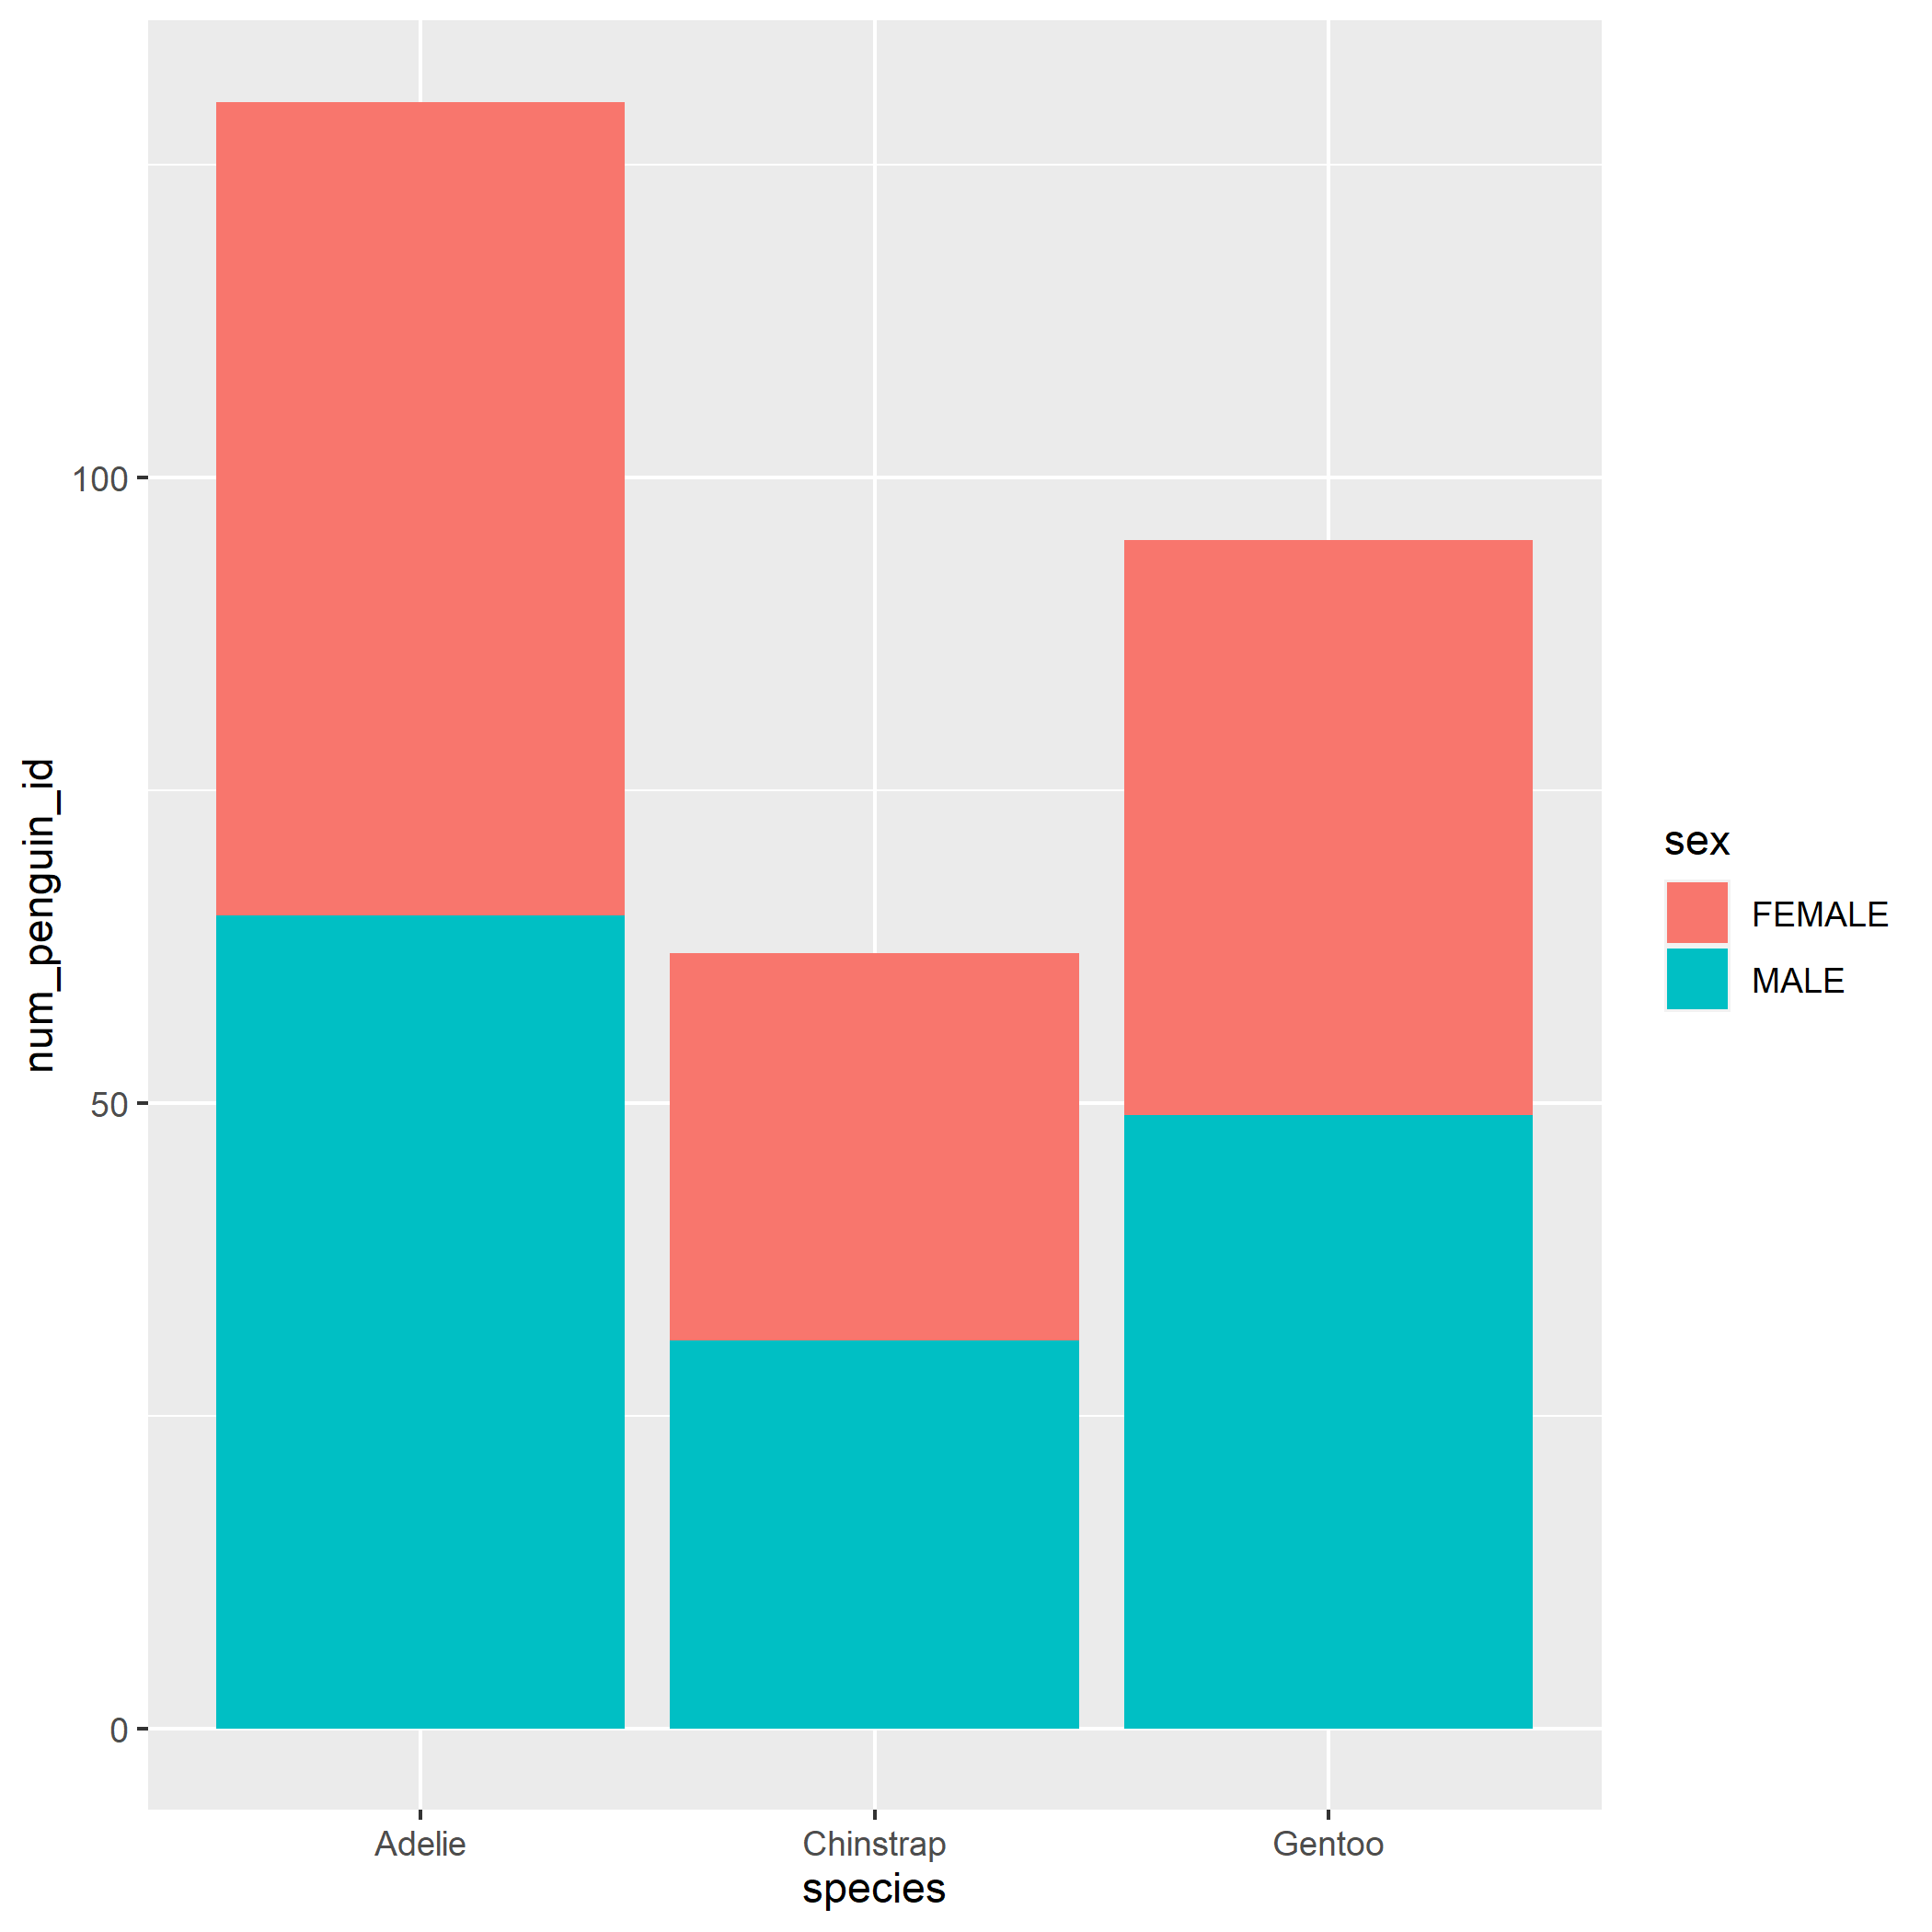
\includegraphics[width=0.8\linewidth]{images/stacked_bar} \caption{A first insight the number of male and female penguins of each species in our study}\label{fig:unnamed-chunk-82}
\end{figure}

We will cover how ggplot works in more detail next week. But in brief, to get the graph we first use the \texttt{ggplot} function, we give \texttt{ggplot} the `aesthetic mappings' of the plot, the values we wish to assign to the x axis, y axis and how we want to ``fill in'' the objects we will draw.

This first line of code will just draw a blank plot, with the \emph{plus} + sign we signify that we want to add a new layer, this builds on top of the first layer and by specifying the function \texttt{geom\_col} we request columns are layered onto the plot. This layer inherits all of the specifications of x,y and fill from \texttt{ggplot()}. And it produces a handy legend.

\hypertarget{challenge}{%
\subsection{Challenge}\label{challenge}}

\begin{rmdquestion}
Can you write and run a script, with appropriate comments, that produces
a summary tibble and graph for the number of penguins of each species,
on the three study islands?
\end{rmdquestion}

\hypertarget{distributions}{%
\section{Distributions}\label{distributions}}

We now know how many penguins were surveyed. Let's move on to look at some distributions. One of our interests was the size of bill lengths, so let's look at the distribution of values in this variable.

Looking at frequency distributions is very \emph{useful} because it shows the shape of the \emph{sample distribution}, that shape is very important for the types of formal statistics we can do later.

Here is the script to plot frequency distribution, as before we pipe the data into ggplot. This time we only specify an x variable because we intend to plot a histogram and the y variable is always the count of observations. We then ask for the data to be presented in 50 equally sized bins of data. So in this case we have chopped the range of the x axis into 50 equal parts and counted the number of observations that fall within each one.

\begin{Shaded}
\begin{Highlighting}[]
\NormalTok{penguins }\SpecialCharTok{\%\textgreater{}\%} 
  \FunctionTok{ggplot}\NormalTok{(}\FunctionTok{aes}\NormalTok{(}\AttributeTok{x=}\NormalTok{culmen\_length\_mm))}\SpecialCharTok{+}
  \FunctionTok{geom\_histogram}\NormalTok{(}\AttributeTok{bins=}\DecValTok{50}\NormalTok{)}
\end{Highlighting}
\end{Shaded}

\begin{figure}
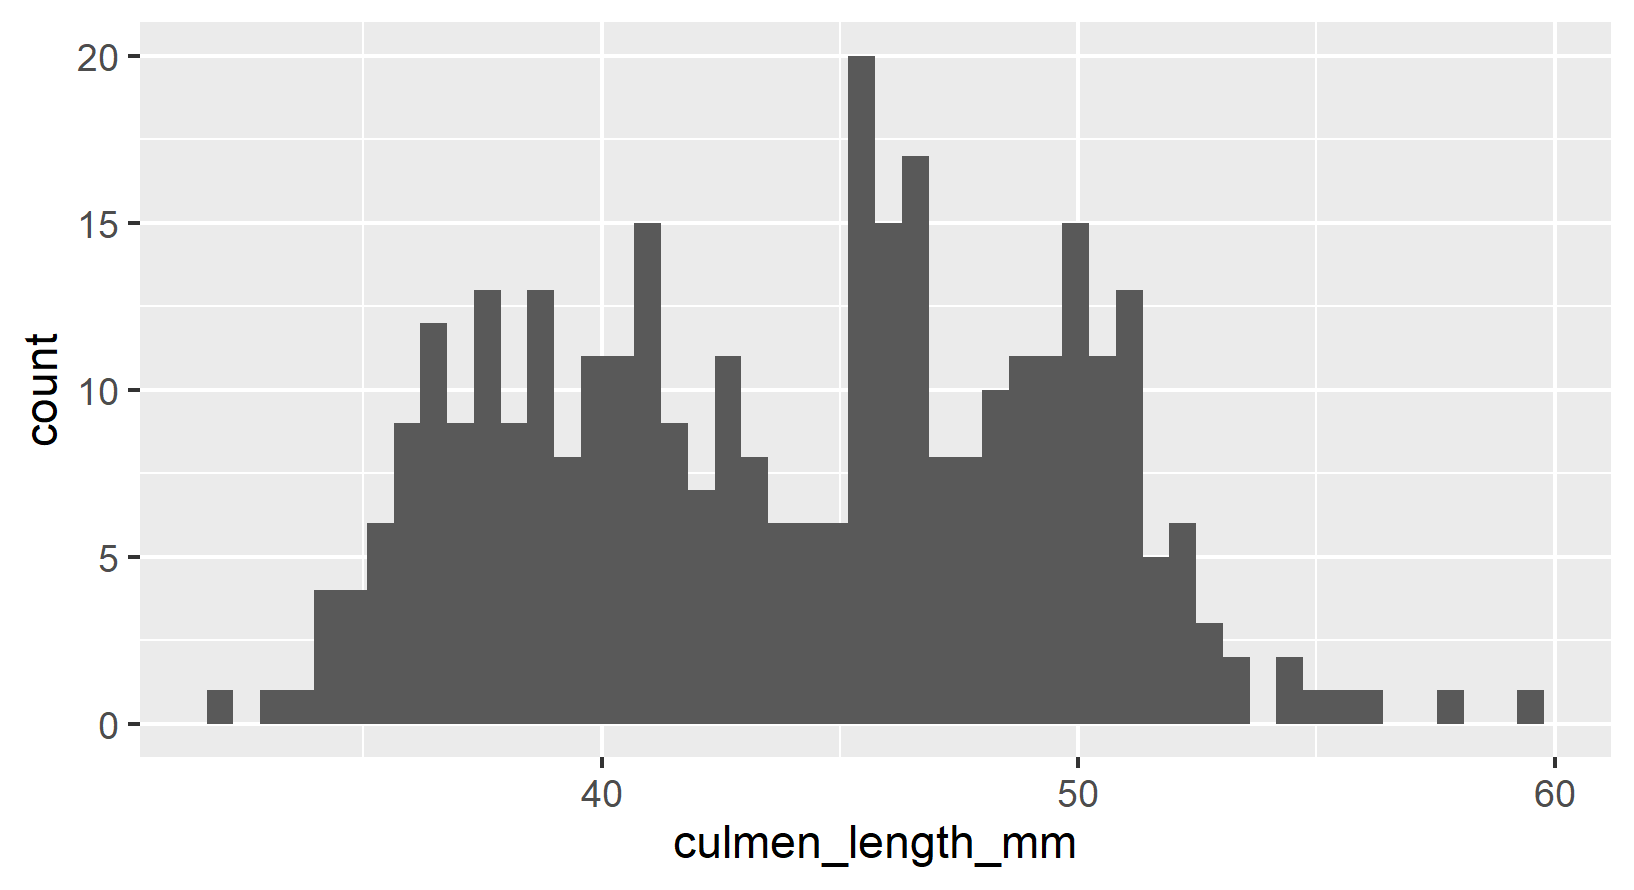
\includegraphics[width=0.8\linewidth]{images/Distribution} \caption{Frequency distribution of culmen length in penguins}\label{fig:unnamed-chunk-85}
\end{figure}

\begin{quote}
** Note - Bins. Have a go at changing the value specified to the bins argument, and observe how the figure changes.
\end{quote}

\hypertarget{insights}{%
\subsection{Insights}\label{insights}}

\begin{rmdquestion}
\begin{itemize}
\item
  Are you surprised at all by the distribution? We have drawn a
  continuous variable from a natural population, what did you expect the
  distribution to look like?
\item
  Can you change the code for the histogram plot to produce
  distributions for each sex?
\item
  How has this changed your interpretation of the distributions?
\end{itemize}
\end{rmdquestion}

\hypertarget{more-distributions}{%
\section{More distributions}\label{more-distributions}}

From the figures you have made, you should be able to make some guesses about the means and medians of the data. But we can use \texttt{dplyr} to get more accurate answers.

\begin{Shaded}
\begin{Highlighting}[]
\CommentTok{\# generate the mean, median and standard deviation of culmen length in three species of penguins}

\NormalTok{penguins }\SpecialCharTok{\%\textgreater{}\%} 
  \FunctionTok{group\_by}\NormalTok{(species) }\SpecialCharTok{\%\textgreater{}\%} 
  \FunctionTok{summarise}\NormalTok{(}\AttributeTok{mean\_culmen\_length=}\FunctionTok{mean}\NormalTok{(culmen\_length\_mm),}
            \AttributeTok{median\_culmen\_length=}\FunctionTok{median}\NormalTok{(culmen\_length\_mm),}
            \AttributeTok{sd\_culmen\_length=}\FunctionTok{sd}\NormalTok{(culmen\_length\_mm))}
\end{Highlighting}
\end{Shaded}

Huh??? What's going on??? We get NAs because there are NAs in our dataset any calculation involving nothing produces nothing. Try this

\begin{Shaded}
\begin{Highlighting}[]
\CommentTok{\# messing about with NA calculations}
\DecValTok{4}\SpecialCharTok{+}\ConstantTok{NA}

\DecValTok{3}\SpecialCharTok{*}\ConstantTok{NA}

\ConstantTok{NA}\SpecialCharTok{\^{}}\DecValTok{2}

\NormalTok{(}\DecValTok{1}\SpecialCharTok{+}\DecValTok{2}\SpecialCharTok{+}\ConstantTok{NA}\NormalTok{)}\SpecialCharTok{/}\DecValTok{2}
\end{Highlighting}
\end{Shaded}

We need to remember to specify the argument to remove \texttt{NA}

\begin{Shaded}
\begin{Highlighting}[]
\CommentTok{\# generate the mean, median and standard deviation of culmen length in three species of penguins}
\CommentTok{\# specify the removal of NA values}
\NormalTok{penguins }\SpecialCharTok{\%\textgreater{}\%} 
  \FunctionTok{group\_by}\NormalTok{(species)}
  \FunctionTok{summarise}\NormalTok{(}\AttributeTok{mean\_culmen\_length=}\FunctionTok{mean}\NormalTok{(culmen\_length\_mm, }\AttributeTok{na.rm=}\ConstantTok{TRUE}\NormalTok{),}
            \AttributeTok{median\_culmen\_length=}\FunctionTok{median}\NormalTok{(culmen\_length\_mm, }\AttributeTok{na.rm=}\ConstantTok{TRUE}\NormalTok{),}
            \AttributeTok{sd\_culmen\_length=}\FunctionTok{sd}\NormalTok{(culmen\_length\_mm, }\AttributeTok{na.rm=}\ConstantTok{TRUE}\NormalTok{))}
\end{Highlighting}
\end{Shaded}

\begin{quote}
The mean and median values for each species are \emph{very} similar, which indicates we do not have much \emph{skew} in our data. This detail is important because statistical analyses make lots of assumptions about the underlying distributions of the data.
\end{quote}

\hypertarget{initial-conclusions}{%
\subsection{Initial conclusions}\label{initial-conclusions}}

In these data we are already able to make some useful insights

\begin{itemize}
\item
  Fewer Chinstrap penguins were surveyed than Adelie or Gentoo's
\item
  The average bill length for Adelie penguins is 38.8 mm, on average 8.7mm shorter than Gentoo's and 10mm shorter than Chinstrap's
\item
  There does not appear to be much difference between Chinstrap and Gentoo bill lengths (on average 1.3mm)
\end{itemize}

These might appear to be modest insights - but have learned several data manipulation and summary techniques. We can also start to take a look at some of our initial hypotheses!!!

\begin{rmdquestion}
\begin{itemize}
\tightlist
\item
  How does this data stack up against the hypothesis about bill
  morphology we put forward last week?
\end{itemize}
\end{rmdquestion}

To make more and conclusive insights we have a bit further to go, but I think you deserve a pat on the back

\begin{Shaded}
\begin{Highlighting}[]
\CommentTok{\# R generate some praise}
\NormalTok{praise}\SpecialCharTok{::}\FunctionTok{praise}\NormalTok{()}
\end{Highlighting}
\end{Shaded}

\hypertarget{data-transformation}{%
\section{Data transformation}\label{data-transformation}}

In the previous section we made some basic insights into observation numbers, distributed by species, sex and location. We also started to gain core insights into some of our central hypotheses, but you have probably noticed we don't actually have a variable on the \texttt{relative\ bill\ lengths/depths}. Why is this important? Well we clearly saw there was a difference in bill lengths between our three species. But we haven't taken into account that some of these species might be very different in body size. Our measure of bill lengths as an indicator of feeding strategy, might be confounded by body size (a bigger penguin is likely to have a bigger bill).

We don't have a variable explicitly called body size. Instead we have to use ``proxies'' suitable proxies might be `flipper length' or `body mass'. Neither is perfect

\begin{itemize}
\tightlist
\item
  Flipper length

  \begin{itemize}
  \tightlist
  \item
    Pros: linked to skeletal structure, constant
  \item
    Cons: relative flipper length could also vary by species
  \end{itemize}
\item
  Body mass

  \begin{itemize}
  \tightlist
  \item
    Pros: more of an indication of central size?
  \item
    Cons: condition dependent, likely to change over the year
  \end{itemize}
\end{itemize}

Let's take a look at the distribution of body mass among our three species.

\begin{Shaded}
\begin{Highlighting}[]
\CommentTok{\# frequency distribution of body mass by species}
\NormalTok{penguins }\SpecialCharTok{\%\textgreater{}\%} 
  \FunctionTok{ggplot}\NormalTok{(}\FunctionTok{aes}\NormalTok{(}\AttributeTok{x=}\NormalTok{body\_mass\_g, }\AttributeTok{fill=}\NormalTok{species))}\SpecialCharTok{+}
  \FunctionTok{geom\_histogram}\NormalTok{(}\AttributeTok{bins=}\DecValTok{50}\NormalTok{)}
\end{Highlighting}
\end{Shaded}

How does the distribution you have found compare with your insights on bill length? We can do this using the \texttt{cor\_test} function from the package \texttt{rstatix} (\citet{R-rstatix}). This package contains a number of `pipe-friendly' simple statistics functions

Add the \texttt{library()} for \texttt{rstatix} at the \textbf{top} of your RScript with an appropriate comment \#

\begin{Shaded}
\begin{Highlighting}[]
\CommentTok{\# a simple correlation test from the rstatix package}
\NormalTok{penguins }\SpecialCharTok{\%\textgreater{}\%} 
  \FunctionTok{group\_by}\NormalTok{(species) }\SpecialCharTok{\%\textgreater{}\%} \CommentTok{\# group by species}
  \FunctionTok{cor\_test}\NormalTok{(body\_mass\_g, culmen\_length\_mm) }\CommentTok{\# correlation between body mass and bill length}
\end{Highlighting}
\end{Shaded}

We can see that these two variables `co-vary' a lot, but this appears to be quite species specific. We can already make the insight that Chinstrap penguins appear to have the shortest bill length relative to body mass.

We can make a new variable that is the `relative size of culmen length compared to flipper length'

\begin{Shaded}
\begin{Highlighting}[]
\CommentTok{\# use mutate to produce a new variable that is a ratio of culmen length to flipper length}
\NormalTok{penguins }\OtherTok{\textless{}{-}}\NormalTok{ penguins }\SpecialCharTok{\%\textgreater{}\%} 
  \FunctionTok{mutate}\NormalTok{(}\AttributeTok{relative\_bill\_length =}\NormalTok{ culmen\_length\_mm}\SpecialCharTok{/}\NormalTok{body\_mass\_g)}
\end{Highlighting}
\end{Shaded}

We are probably also interested in bill depth?

\begin{Shaded}
\begin{Highlighting}[]
\CommentTok{\# use mutate to produce a new variable that is a ratio of culmen depth to flipper length}
\NormalTok{penguins }\OtherTok{\textless{}{-}}\NormalTok{ penguins }\SpecialCharTok{\%\textgreater{}\%} 
  \FunctionTok{mutate}\NormalTok{(}\AttributeTok{relative\_bill\_depth =}\NormalTok{ culmen\_depth\_mm}\SpecialCharTok{/}\NormalTok{body\_mass\_g)}

\CommentTok{\# check that these new variables have been included in the dataset}
\NormalTok{penguins }\SpecialCharTok{\%\textgreater{}\%} 
  \FunctionTok{names}\NormalTok{()}
\end{Highlighting}
\end{Shaded}

\hypertarget{developing-insights}{%
\section{Developing insights}\label{developing-insights}}

First let's focus on the distributions of four variables of interest. Then we will progress on to look at their relationships and differences

\begin{itemize}
\item
  relative\_bill\_length
\item
  relative\_bill\_depth
\item
  delta\_15n
\item
  delta\_13c
\end{itemize}

\hypertarget{distributions-of-the-relative-bill-length}{%
\subsection{Distributions of the relative bill length}\label{distributions-of-the-relative-bill-length}}

We will examine the shape of the \emph{sample distribution} of the data again by using histograms.

\begin{Shaded}
\begin{Highlighting}[]
\CommentTok{\# frequency distribution of relative bill length by species}
\CommentTok{\# we already know we are interested in looking at the distributions \textquotesingle{}within\textquotesingle{} each species}
\NormalTok{penguins }\SpecialCharTok{\%\textgreater{}\%} 
  \FunctionTok{ggplot}\NormalTok{(}\FunctionTok{aes}\NormalTok{(}\AttributeTok{x=}\NormalTok{relative\_bill\_length, }\AttributeTok{fill=}\NormalTok{species))}\SpecialCharTok{+}
  \FunctionTok{geom\_histogram}\NormalTok{(}\AttributeTok{bins=}\DecValTok{50}\NormalTok{)}
\end{Highlighting}
\end{Shaded}

\begin{figure}
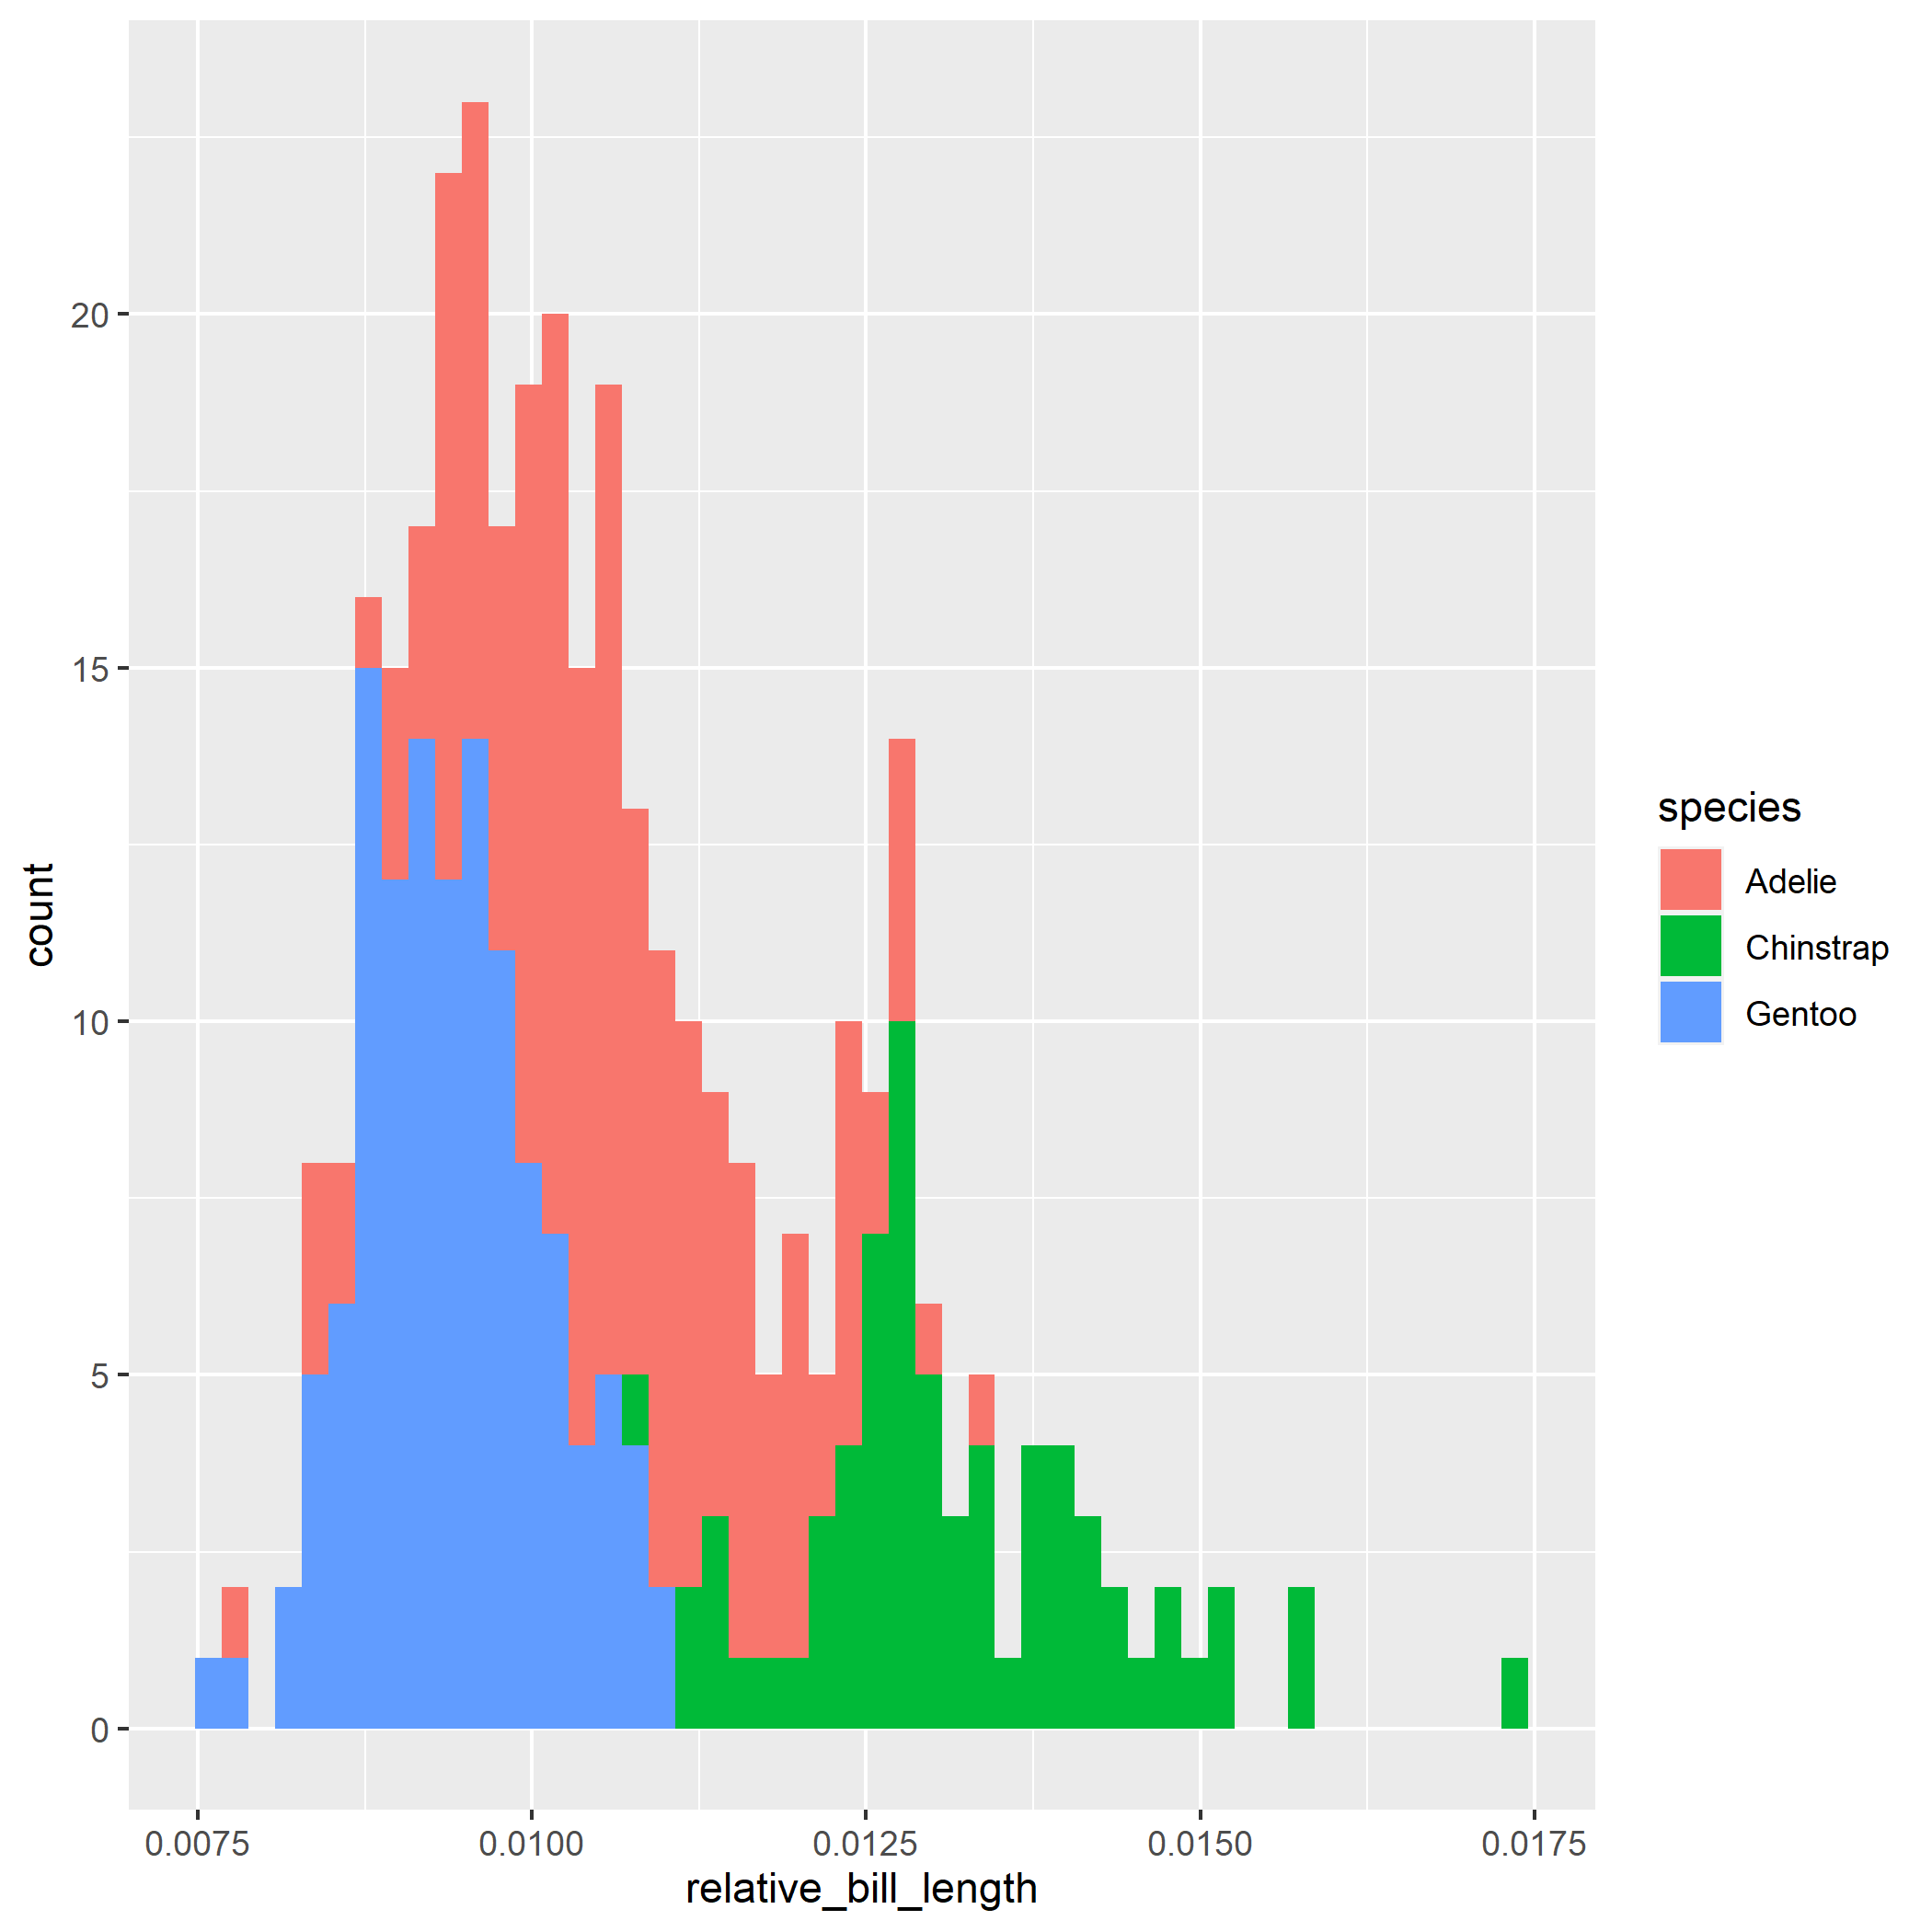
\includegraphics[width=0.8\linewidth]{images/bill_length_distribution} \caption{Frequency distribution of relative bill length in three species of penguins, Adelie, Chinstrap and Gentoo}\label{fig:unnamed-chunk-97}
\end{figure}

Important questions, what shape is the distribution?

\begin{itemize}
\item
  First there must be a lower limit of zero (penguins cannot have negative length bills), does this lead to any truncating of the expected normal distribution bell curve? It doesn't look it.
\item
  Is it symmetrical? Mostly.
\end{itemize}

If it's a little difficult to see - we can separate out these figures using the handy function \texttt{facet\_wrap}

\begin{Shaded}
\begin{Highlighting}[]
\CommentTok{\# frequency distribution of relative bill length by species}
\CommentTok{\# we already know we are interested in looking at the distributions \textquotesingle{}within\textquotesingle{} each species}
\NormalTok{penguins }\SpecialCharTok{\%\textgreater{}\%} 
  \FunctionTok{ggplot}\NormalTok{(}\FunctionTok{aes}\NormalTok{(}\AttributeTok{x=}\NormalTok{relative\_bill\_length, }\AttributeTok{fill=}\NormalTok{species))}\SpecialCharTok{+}
  \FunctionTok{geom\_histogram}\NormalTok{(}\AttributeTok{bins=}\DecValTok{50}\NormalTok{)}\SpecialCharTok{+}
  \FunctionTok{facet\_wrap}\NormalTok{(}\SpecialCharTok{\textasciitilde{}}\NormalTok{species) }\CommentTok{\# facet wrap to look at the separate species more easily}
\end{Highlighting}
\end{Shaded}

\textbackslash begin\{figure\}
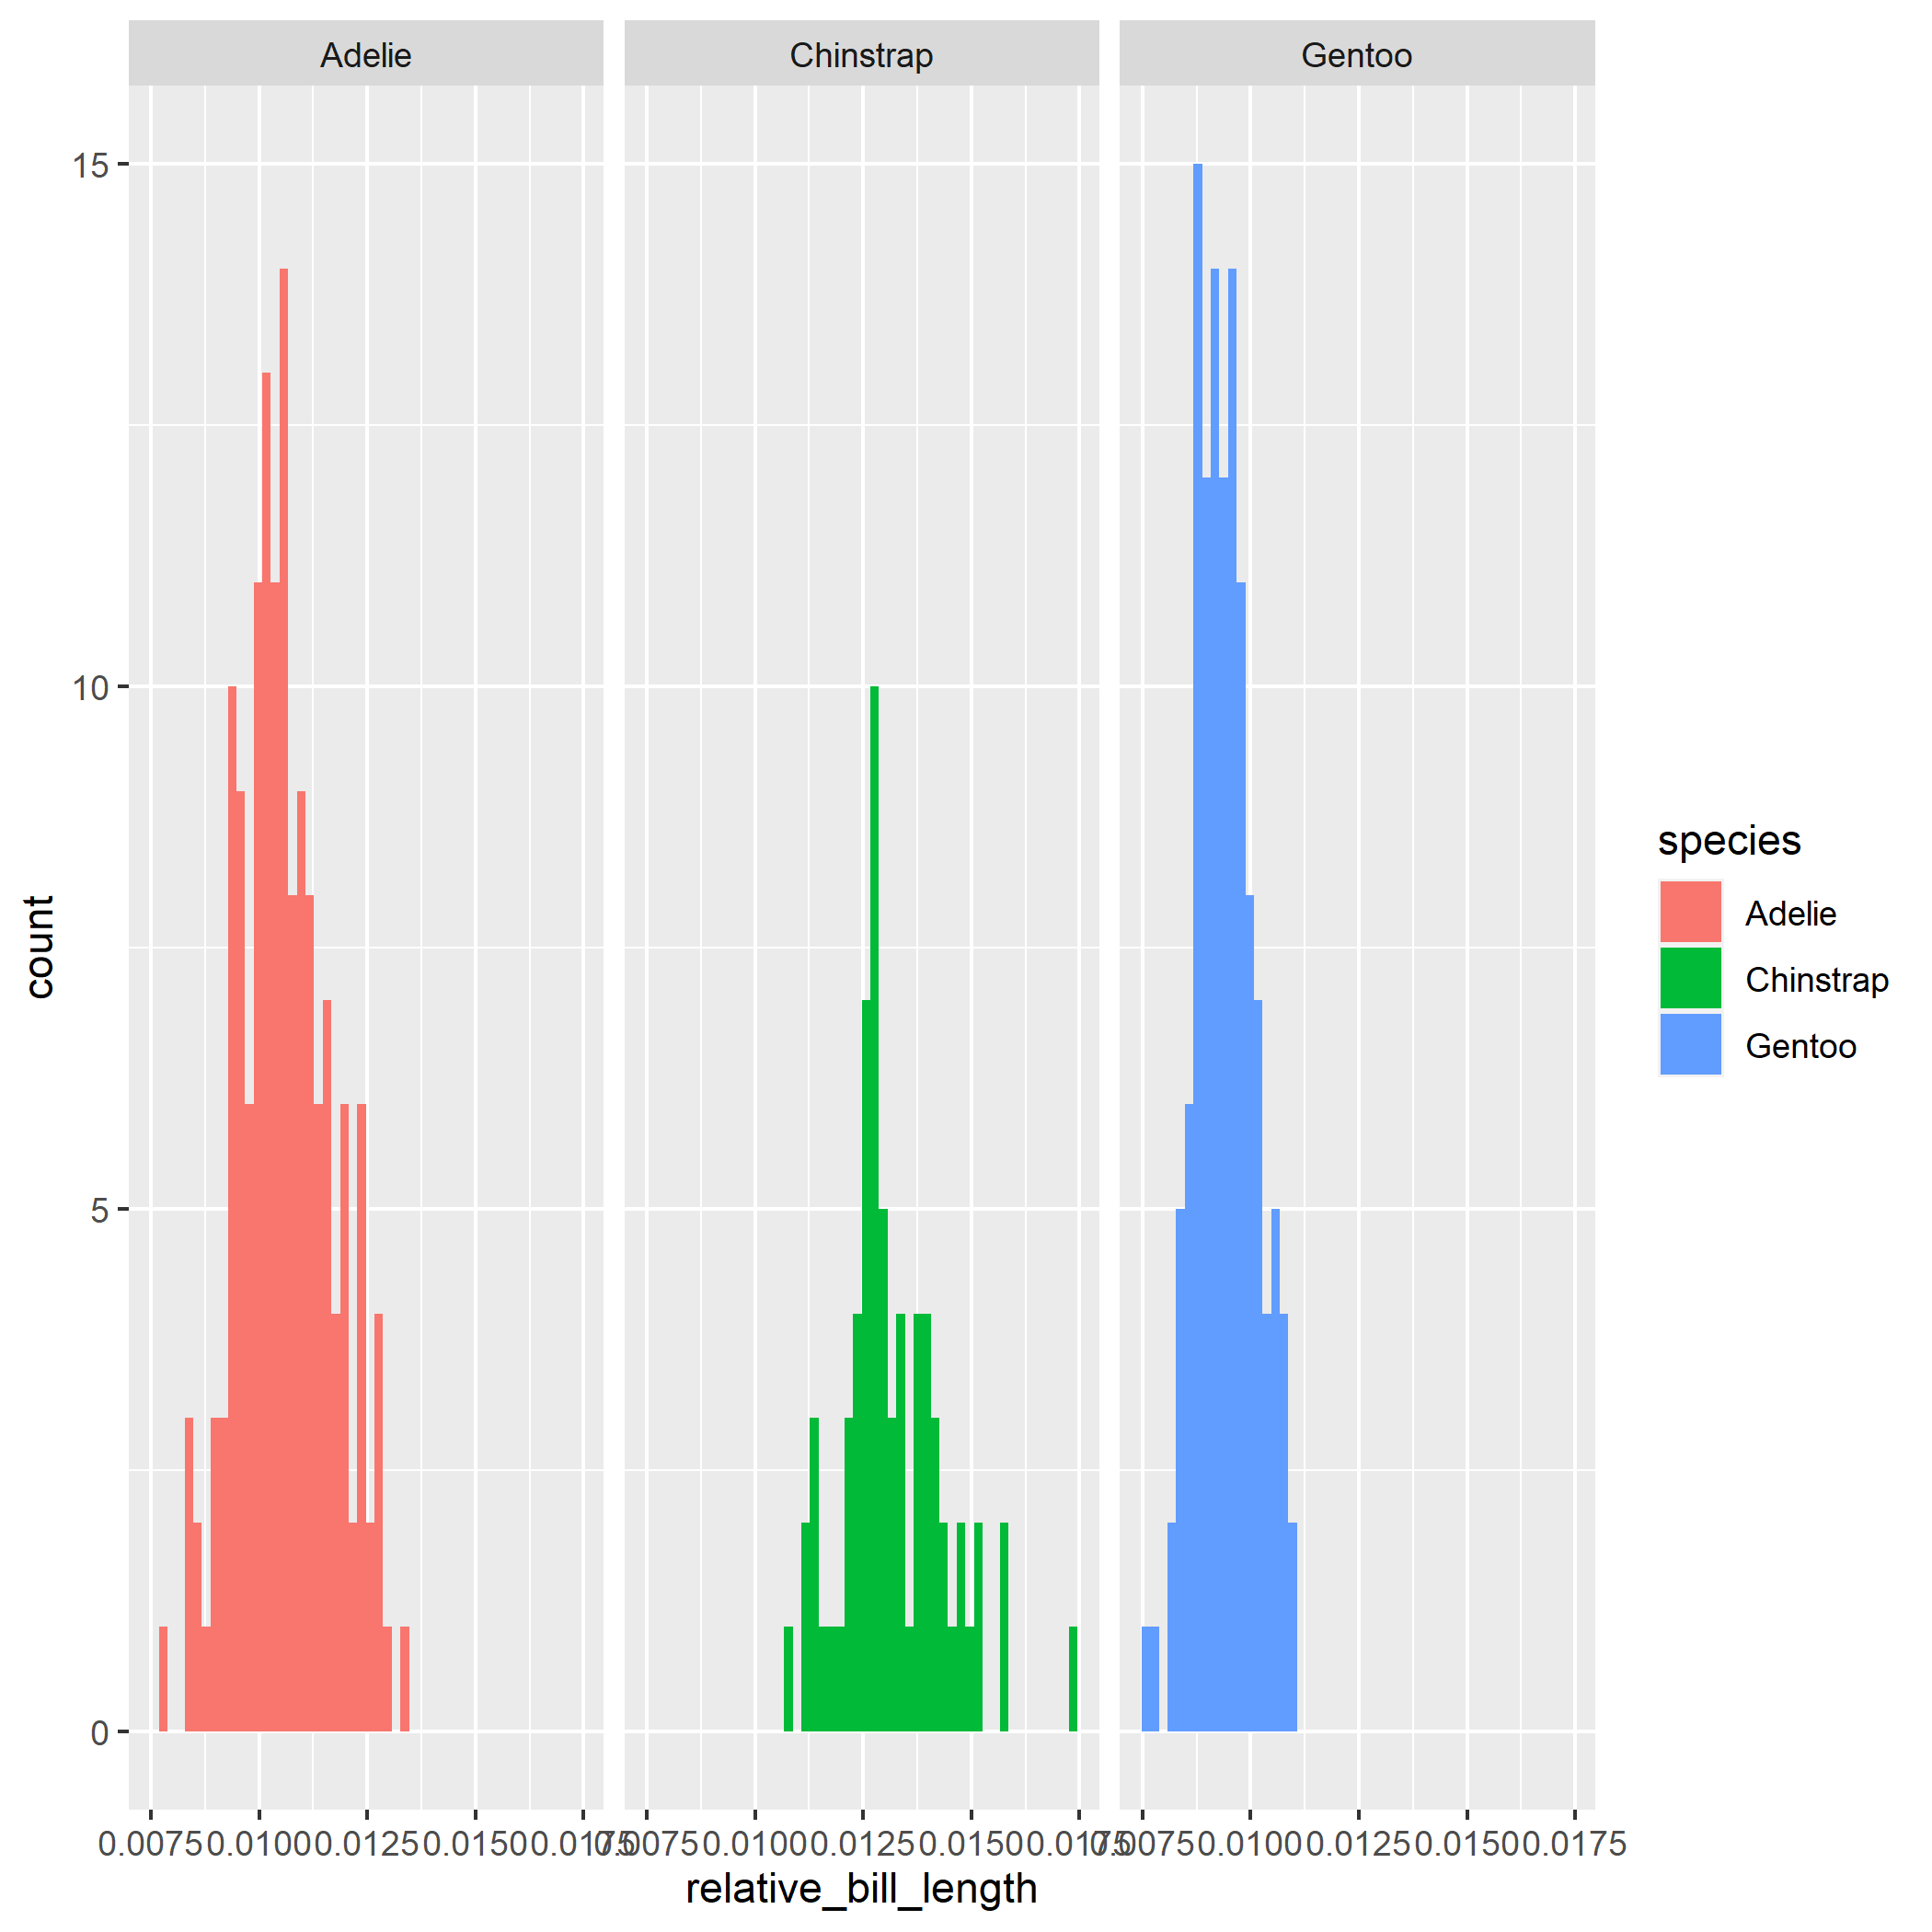
\includegraphics[width=1\linewidth]{images/facetdistribution} \textbackslash caption\{Frequency distribution of relative bill length in three species of penguins, Adelie, Chinstrap and Gentoo - histograms split into three panes by facet\_wrap\}\label{fig:unnamed-chunk-99}
\textbackslash end\{figure\}

\begin{rmdquestion}
Looking at these distributions, how do you think the mean \& median
values will compare in these three species? Think about it first - then
run the code below.
\end{rmdquestion}

\begin{Shaded}
\begin{Highlighting}[]
\CommentTok{\# Mean and Median summaries}
\NormalTok{penguins }\SpecialCharTok{\%\textgreater{}\%} 
  \FunctionTok{group\_by}\NormalTok{(species) }\SpecialCharTok{\%\textgreater{}\%} 
  \FunctionTok{summarise}\NormalTok{(}\AttributeTok{mean\_relative\_bill\_length=}\FunctionTok{mean}\NormalTok{(relative\_bill\_length, }\AttributeTok{na.rm=}\ConstantTok{TRUE}\NormalTok{),}
            \AttributeTok{median\_relative\_bill\_length=}\FunctionTok{median}\NormalTok{(relative\_bill\_length, }\AttributeTok{na.rm=}\ConstantTok{TRUE}\NormalTok{))}
\end{Highlighting}
\end{Shaded}

\begin{verbatim}
# A tibble: 3 x 3
  species   mean_relative_bill_length median_relative_bill_length
  <chr>                         <dbl>                       <dbl>
1 Adelie                      0.0106                      0.0105 
2 Chinstrap                   0.0132                      0.0129 
3 Gentoo                      0.00941                     0.00939
\end{verbatim}

We can see that the mean and median values are almost identical for each species. This indicates we \emph{aren't} dealing with a lot of skew, this is important for when using statistics, which are based on a lot of assumptions like normal distribution.

\begin{rmdquestion}
Can you \textbf{repeat} these steps for the variable
\texttt{relative\_bill\_depth}, \texttt{delta\_15n} and
\texttt{delta\_13c} - add all appropriate comments and commands to your
R Script.
\end{rmdquestion}

\hypertarget{relationshipdifferences}{%
\section{Relationship/differences}\label{relationshipdifferences}}

Getting proper data insights involves looking for relationships or differences.
Remember, if we have a manipulated variable in a well-designed experiment, we may be able to identify a causal effect. With a study without this manipulation, like this penguin study - we cannot be sure any relationships or differences are causal. We have to include some caution in our interpretations.

\hypertarget{differences}{%
\subsection{Differences}\label{differences}}

We have already looked at frequency distributions of the data, where it is possible to see differences. However we can use ggplot and \texttt{geom\_point} to produce difference plots.

\begin{Shaded}
\begin{Highlighting}[]
\CommentTok{\# specifying position with a jitter argument positions points randomly across the x axis this prevents overcrowding}
\NormalTok{penguins }\SpecialCharTok{\%\textgreater{}\%} 
    \FunctionTok{ggplot}\NormalTok{(}\FunctionTok{aes}\NormalTok{(}\AttributeTok{x=}\NormalTok{species, }
               \AttributeTok{y=}\NormalTok{culmen\_length\_mm, }
               \AttributeTok{colour=}\NormalTok{species))}\SpecialCharTok{+} \CommentTok{\# some geoms use color rather than fill to specify colour}
    \FunctionTok{geom\_point}\NormalTok{(}\AttributeTok{position=}\FunctionTok{position\_jitter}\NormalTok{(}\AttributeTok{width=}\FloatTok{0.2}\NormalTok{)) }
\end{Highlighting}
\end{Shaded}

\begin{figure}
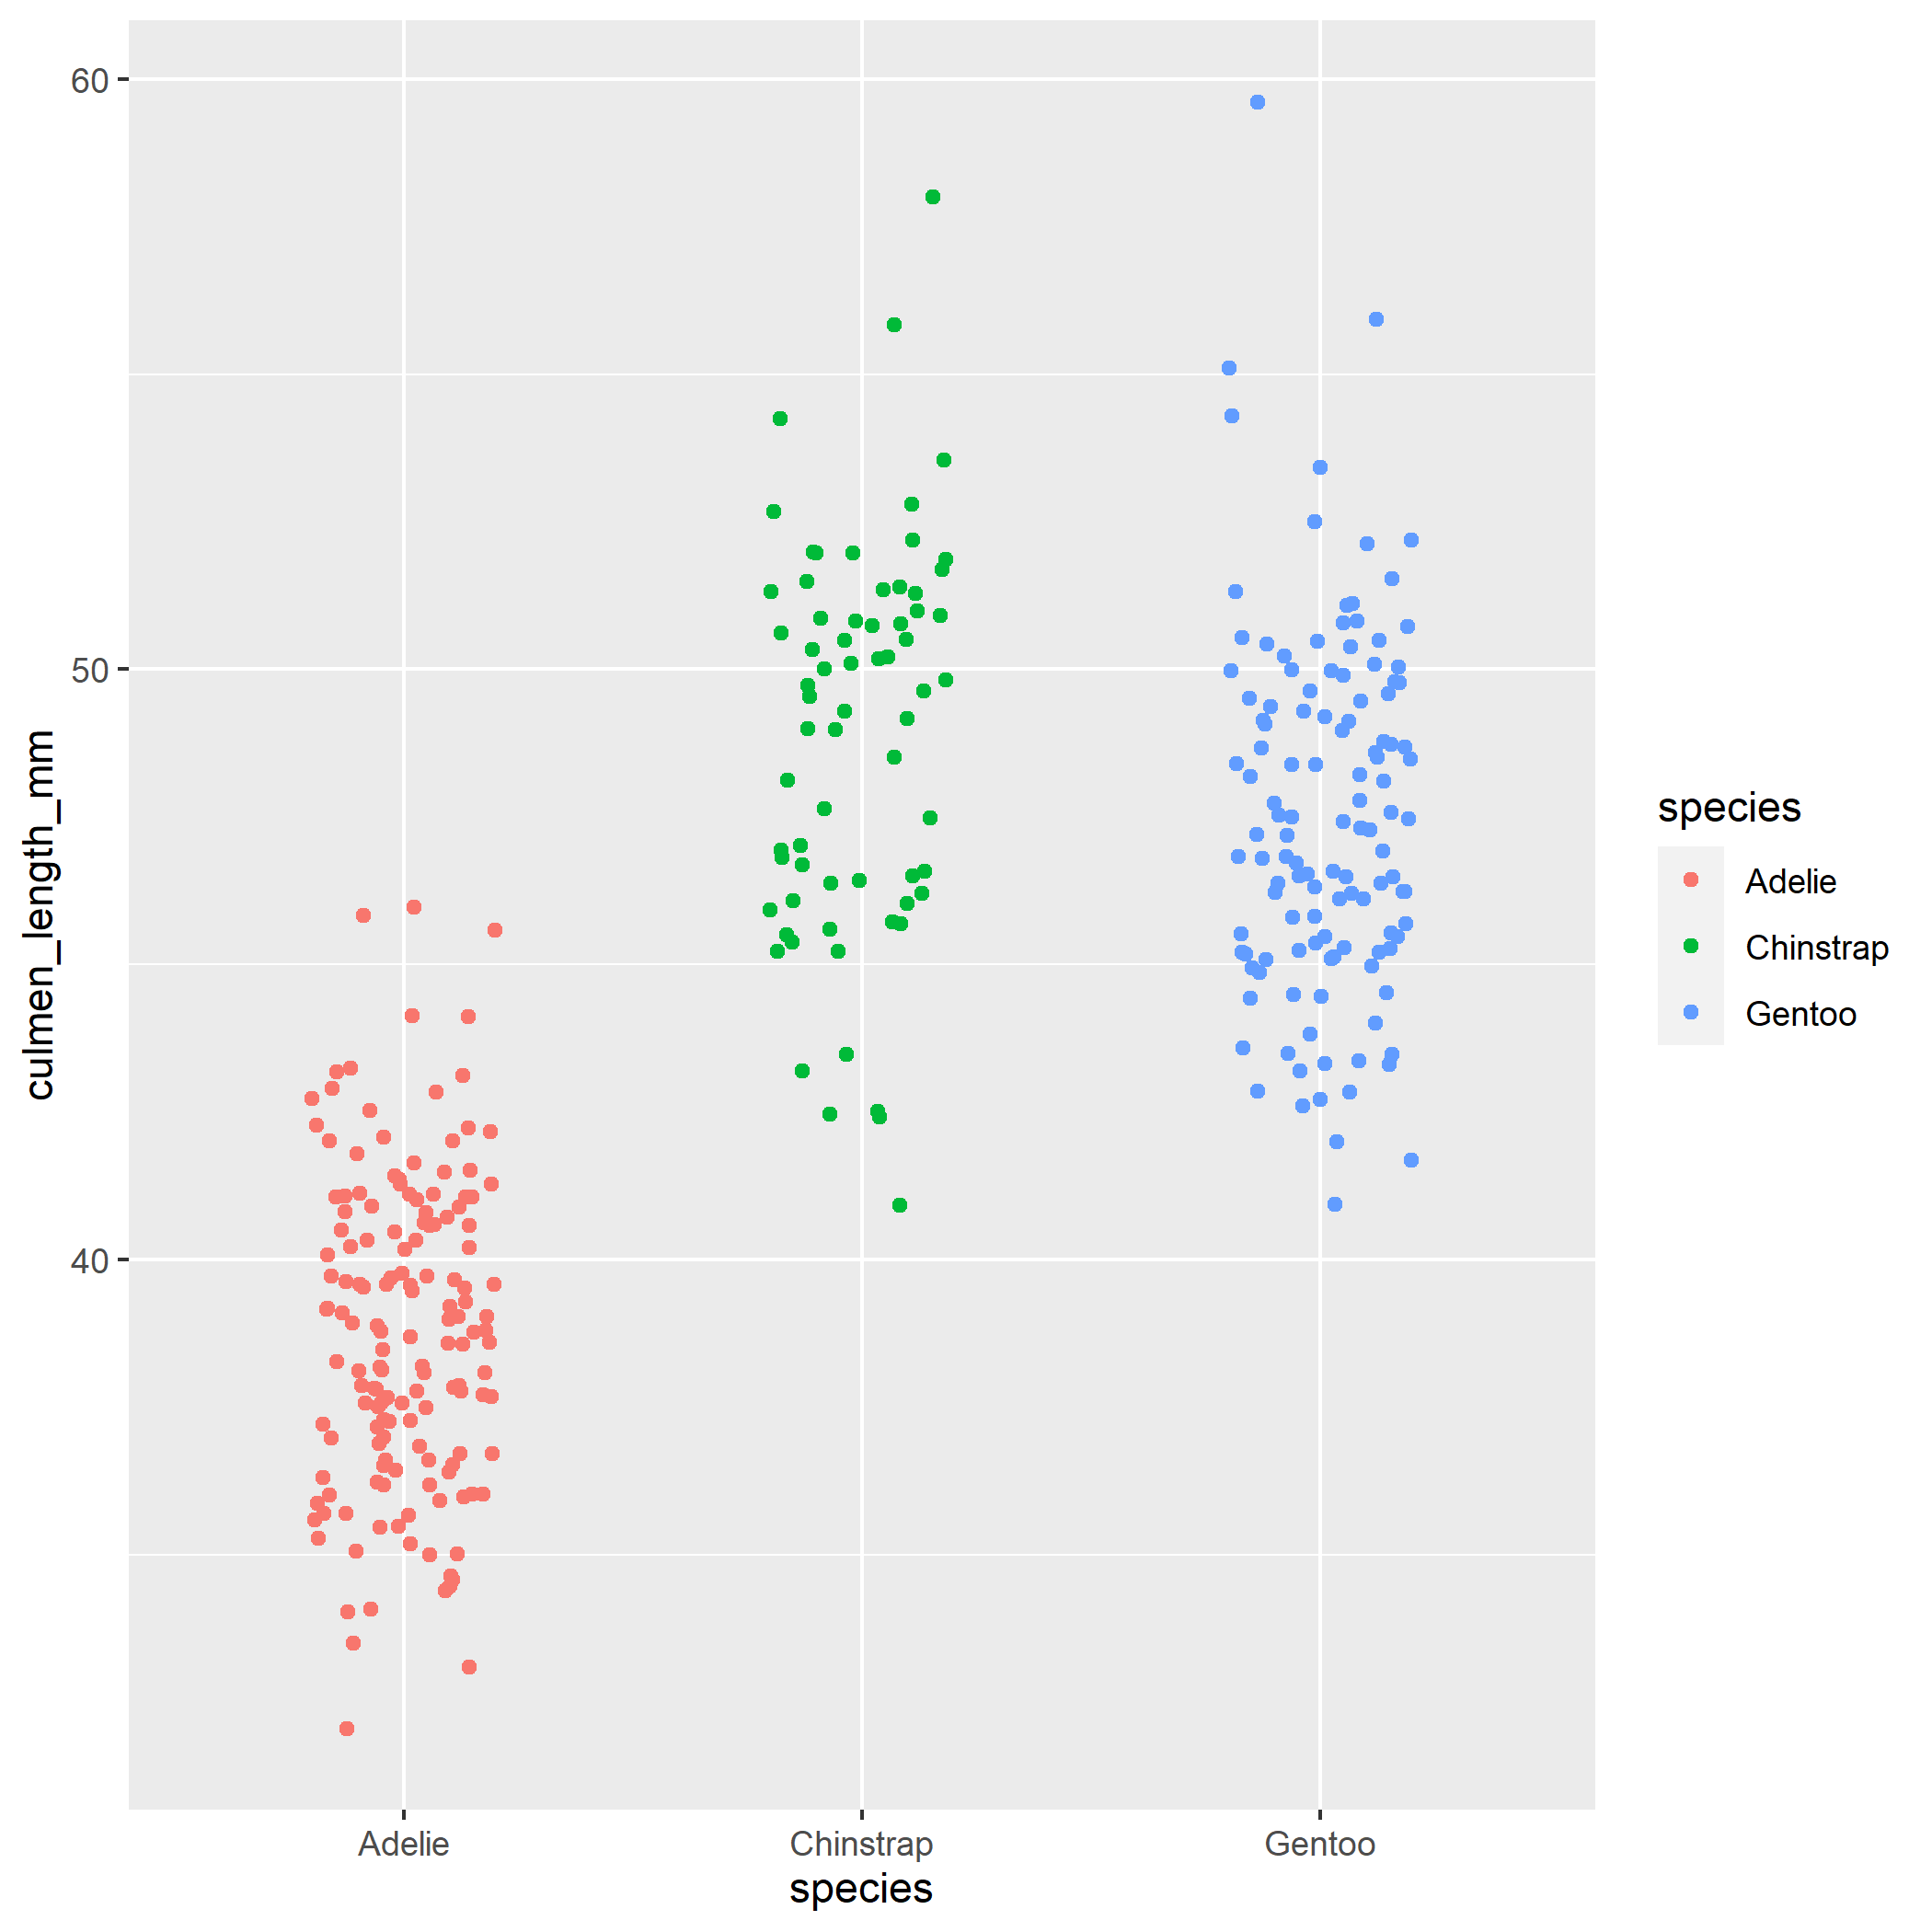
\includegraphics[width=1\linewidth]{images/jitterplot} \caption{Differences in relative bill length of three different species of Antarctic Penguin.}\label{fig:unnamed-chunk-104}
\end{figure}

\begin{quote}
**Note - try altering the width argument and see how it affects the output of the plot.
We will do a deeper dive into ggplot later.
\end{quote}

\begin{rmdquestion}
Try producing these figures for the \texttt{culmen\_depth\_mm},
\texttt{delta\_15n} and \texttt{delta\_13c} variables as well.

What are you observations of the relative differences?
\end{rmdquestion}

\hypertarget{associations}{%
\subsection{Associations}\label{associations}}

It might also be of interest to look at whether any of our variables of interest are strongly associated. For example what is the relationship between heavy carbon/heavy nitrogen isotopes?

\begin{Shaded}
\begin{Highlighting}[]
\NormalTok{penguins }\SpecialCharTok{\%\textgreater{}\%} 
    \FunctionTok{ggplot}\NormalTok{(}\FunctionTok{aes}\NormalTok{(}\AttributeTok{x=}\NormalTok{delta\_15n, }\AttributeTok{y=}\NormalTok{delta\_13c, }\AttributeTok{colour=}\NormalTok{species))}\SpecialCharTok{+}
    \FunctionTok{geom\_point}\NormalTok{()}\SpecialCharTok{+}
    \FunctionTok{geom\_smooth}\NormalTok{(}\AttributeTok{method=}\StringTok{"lm"}\NormalTok{, }\CommentTok{\# produces a simple regression line}
                \AttributeTok{se=}\ConstantTok{FALSE}\NormalTok{)    }\CommentTok{\# no standard error intervals}
\end{Highlighting}
\end{Shaded}

\begin{figure}
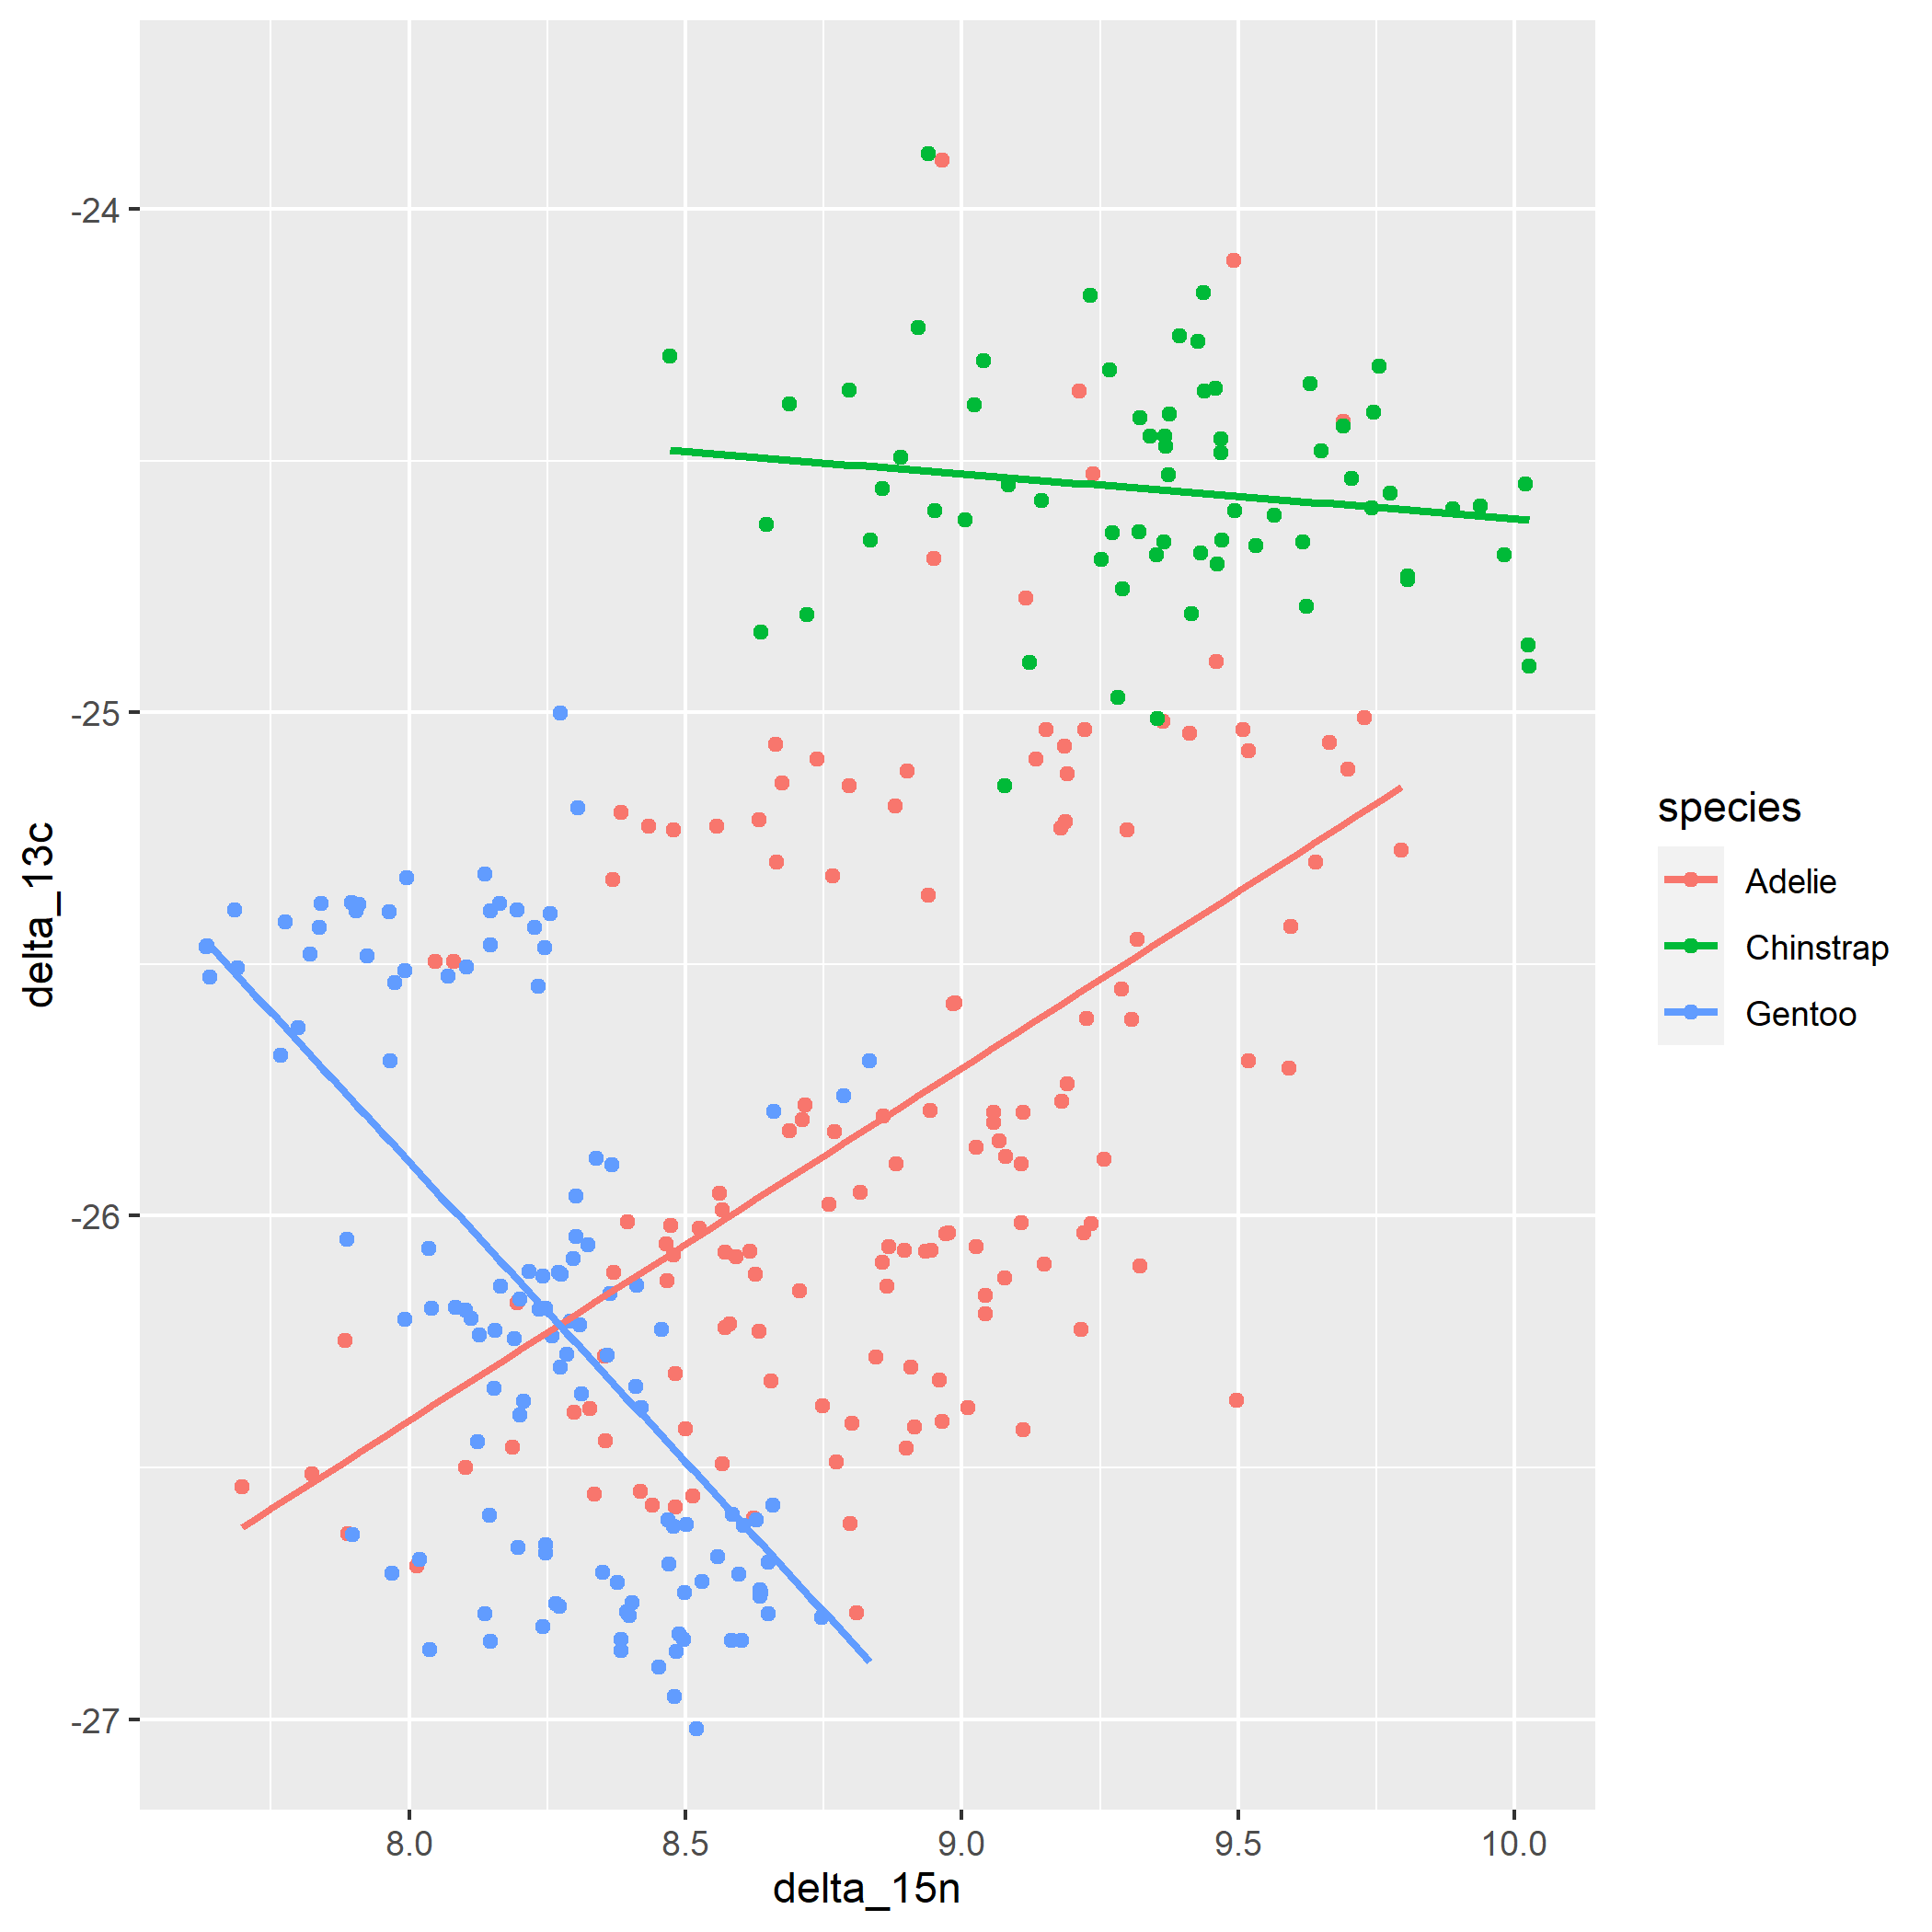
\includegraphics[width=1\linewidth]{images/corrplot} \caption{Asssocation between heavy Nitrogen and heavy Carbon isotopes in blood samples from three Antarctic Penguin species}\label{fig:unnamed-chunk-107}
\end{figure}

We can see here that the association between these isotopes varies a lot by different species, there is probably quite a complex relationship here. It also indicates we should probably investigate these two isotopes separately.

\begin{itemize}
\tightlist
\item
  Have a look at the relative bill length and depth relationships as well
\end{itemize}

\hypertarget{sex-interactions}{%
\section{Sex interactions}\label{sex-interactions}}

Now let's concern ourselves with interactions. We have \emph{already} seen how our interpretation of certain variables can be heavily altered if we don't take into account important contexts - like morphology in relation to species.

Thinking about sensible interactions takes patience and good biological understanding, the payoff is it can produce unique insights.

Focusing on relative bill length, we have seen there are differences between species, however we have not considered the potential association of sex. In many species males and females are `dimorphic' and this has the potential to influence our observations if:

\begin{itemize}
\item
  sex has a substantial/bigger effect on morphology than species
\item
  uneven numbers of males/females were scored in our studies
\end{itemize}

Using \texttt{summarise} \texttt{group\_by} and \texttt{n\_distinct} you should quickly be able to check the numbers of males and females surveyed within each species.

\begin{verbatim}
# A tibble: 6 x 3
# Groups:   species [3]
  species   sex    num_penguin_id
  <chr>     <chr>           <int>
1 Adelie    FEMALE             65
2 Adelie    MALE               65
3 Chinstrap FEMALE             31
4 Chinstrap MALE               31
5 Gentoo    FEMALE             46
6 Gentoo    MALE               49
\end{verbatim}

Looks like numbers are even, which is good. Again focusing on relative bill length let's generate some figures breaking down this variable by sex and species.

First let's generate some more simple summary stats - this time we are assigning it to an object to use later

\begin{Shaded}
\begin{Highlighting}[]
\NormalTok{penguin\_stats }\OtherTok{\textless{}{-}}\NormalTok{ penguins }\SpecialCharTok{\%\textgreater{}\%} 
  \FunctionTok{group\_by}\NormalTok{(sex, species) }\SpecialCharTok{\%\textgreater{}\%} 
  \FunctionTok{summarise}\NormalTok{(}\AttributeTok{mean\_relative\_bill\_length=}\FunctionTok{mean}\NormalTok{(relative\_bill\_length, }\AttributeTok{na.rm=}\ConstantTok{TRUE}\NormalTok{))}
\end{Highlighting}
\end{Shaded}

Now we are going to make our first figure which includes both raw and summary data. Copy and run the code below, and see if you can add comments next to the arguments you are unfamiliar with about what they might be doing.

\begin{Shaded}
\begin{Highlighting}[]
\NormalTok{penguins }\SpecialCharTok{\%\textgreater{}\%} 
  \FunctionTok{drop\_na}\NormalTok{(sex) }\SpecialCharTok{\%\textgreater{}\%} 
  \FunctionTok{ggplot}\NormalTok{(}\FunctionTok{aes}\NormalTok{(}\AttributeTok{x=}\NormalTok{sex, }
             \AttributeTok{y=}\NormalTok{relative\_bill\_length))}\SpecialCharTok{+}
  \FunctionTok{geom\_jitter}\NormalTok{(}\AttributeTok{position=}\FunctionTok{position\_jitter}\NormalTok{(}\AttributeTok{width=}\FloatTok{0.2}\NormalTok{), }
              \AttributeTok{alpha=}\FloatTok{0.4}\NormalTok{)}\SpecialCharTok{+}
  \FunctionTok{geom\_point}\NormalTok{(}\AttributeTok{data=}\NormalTok{penguin\_stats, }\FunctionTok{aes}\NormalTok{(}\AttributeTok{x=}\NormalTok{sex, }
                                     \AttributeTok{y=}\NormalTok{mean\_relative\_bill\_length), }
             \AttributeTok{size=}\DecValTok{4}\NormalTok{, }
             \AttributeTok{color=}\StringTok{"blue"}\NormalTok{)}\SpecialCharTok{+}
  \FunctionTok{facet\_wrap}\NormalTok{(}\SpecialCharTok{\textasciitilde{}}\NormalTok{species)}
\end{Highlighting}
\end{Shaded}

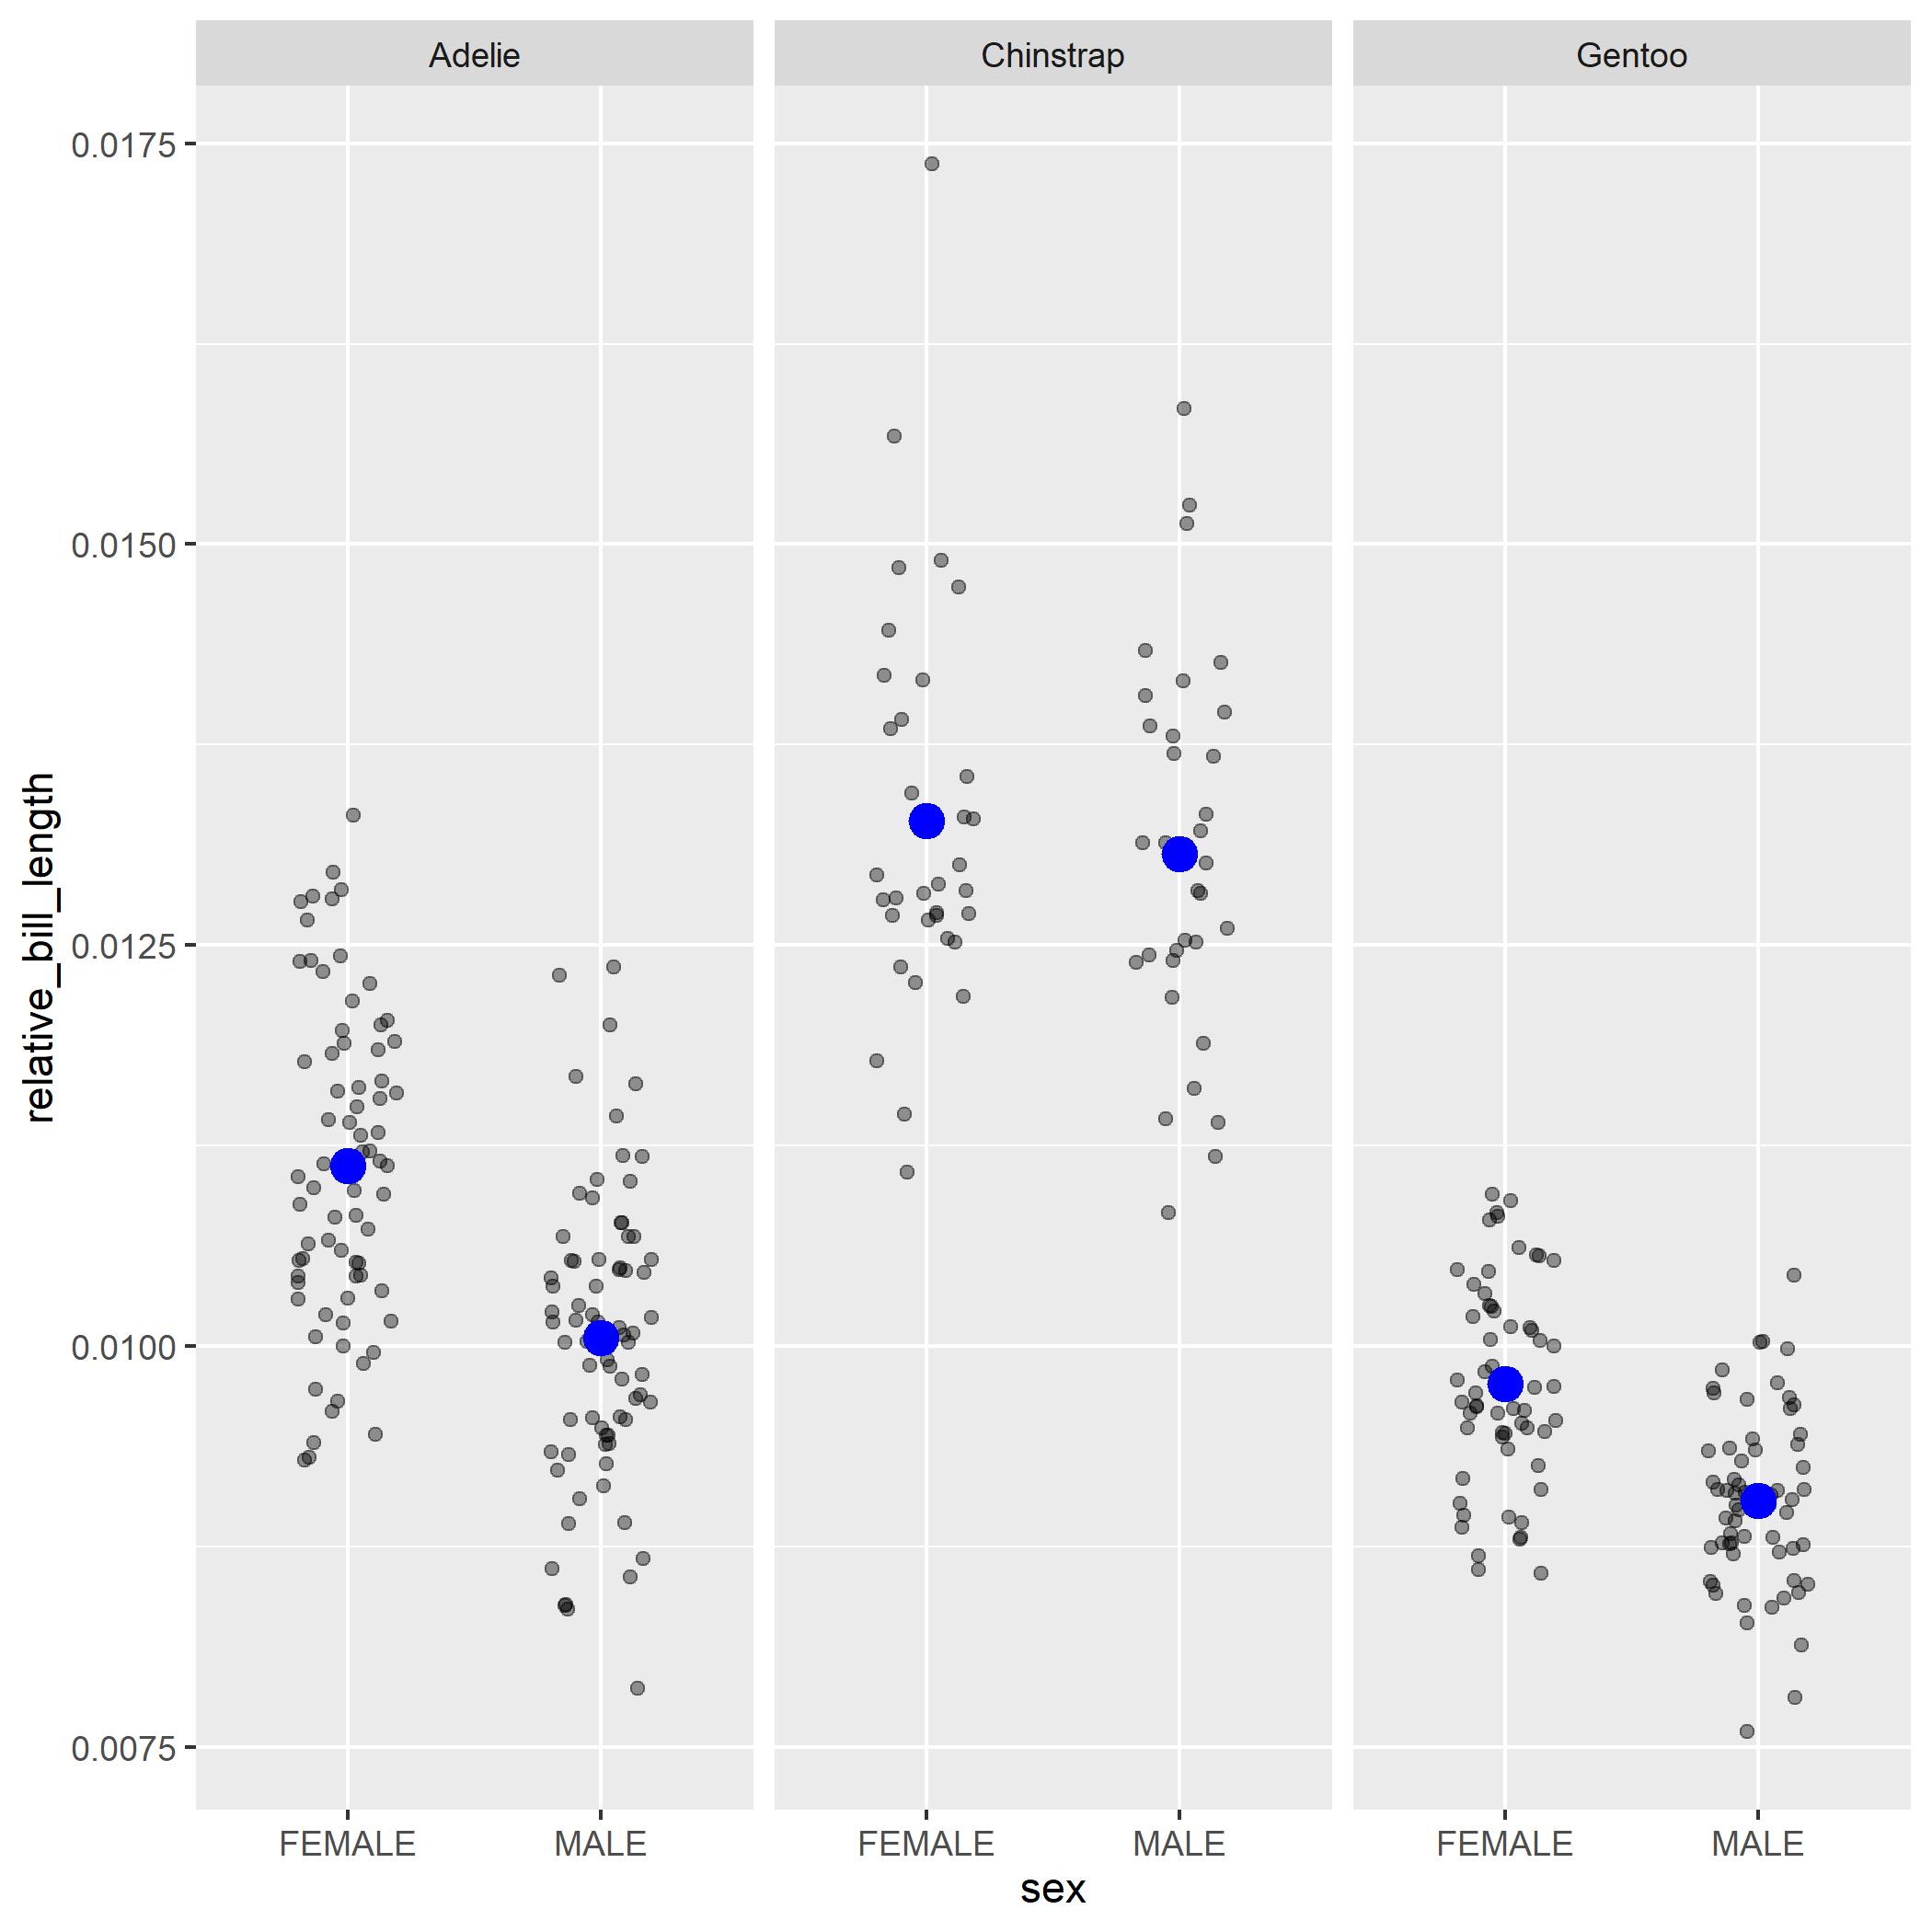
\includegraphics[width=1\linewidth]{images/bluedotplot}
\textgreater{} Note - we could be producing something much simpler, like a box and whisker plot. It is often better to plot the data points rather than summaries of them

Imagine a line connects the two blue dots in each facet, these blue dots are the mean values. The slope of the line (if we drew them) would be downwards from females to males, indicating that on average females are larger. But the slop would not be very large. If we drew slope between \emph{each} of the three female averages these would be much steeper. So we can say that size `on average' varies more \emph{between} species than \emph{between} sexes.

See if you can make figures for all four of our variables of interest, then compare them to our initial hypotheses.

At this stage we do not have enough evidence to formally ``reject'' any of our null hypotheses, however we can describe the trends which appear to be present.

\begin{figure}
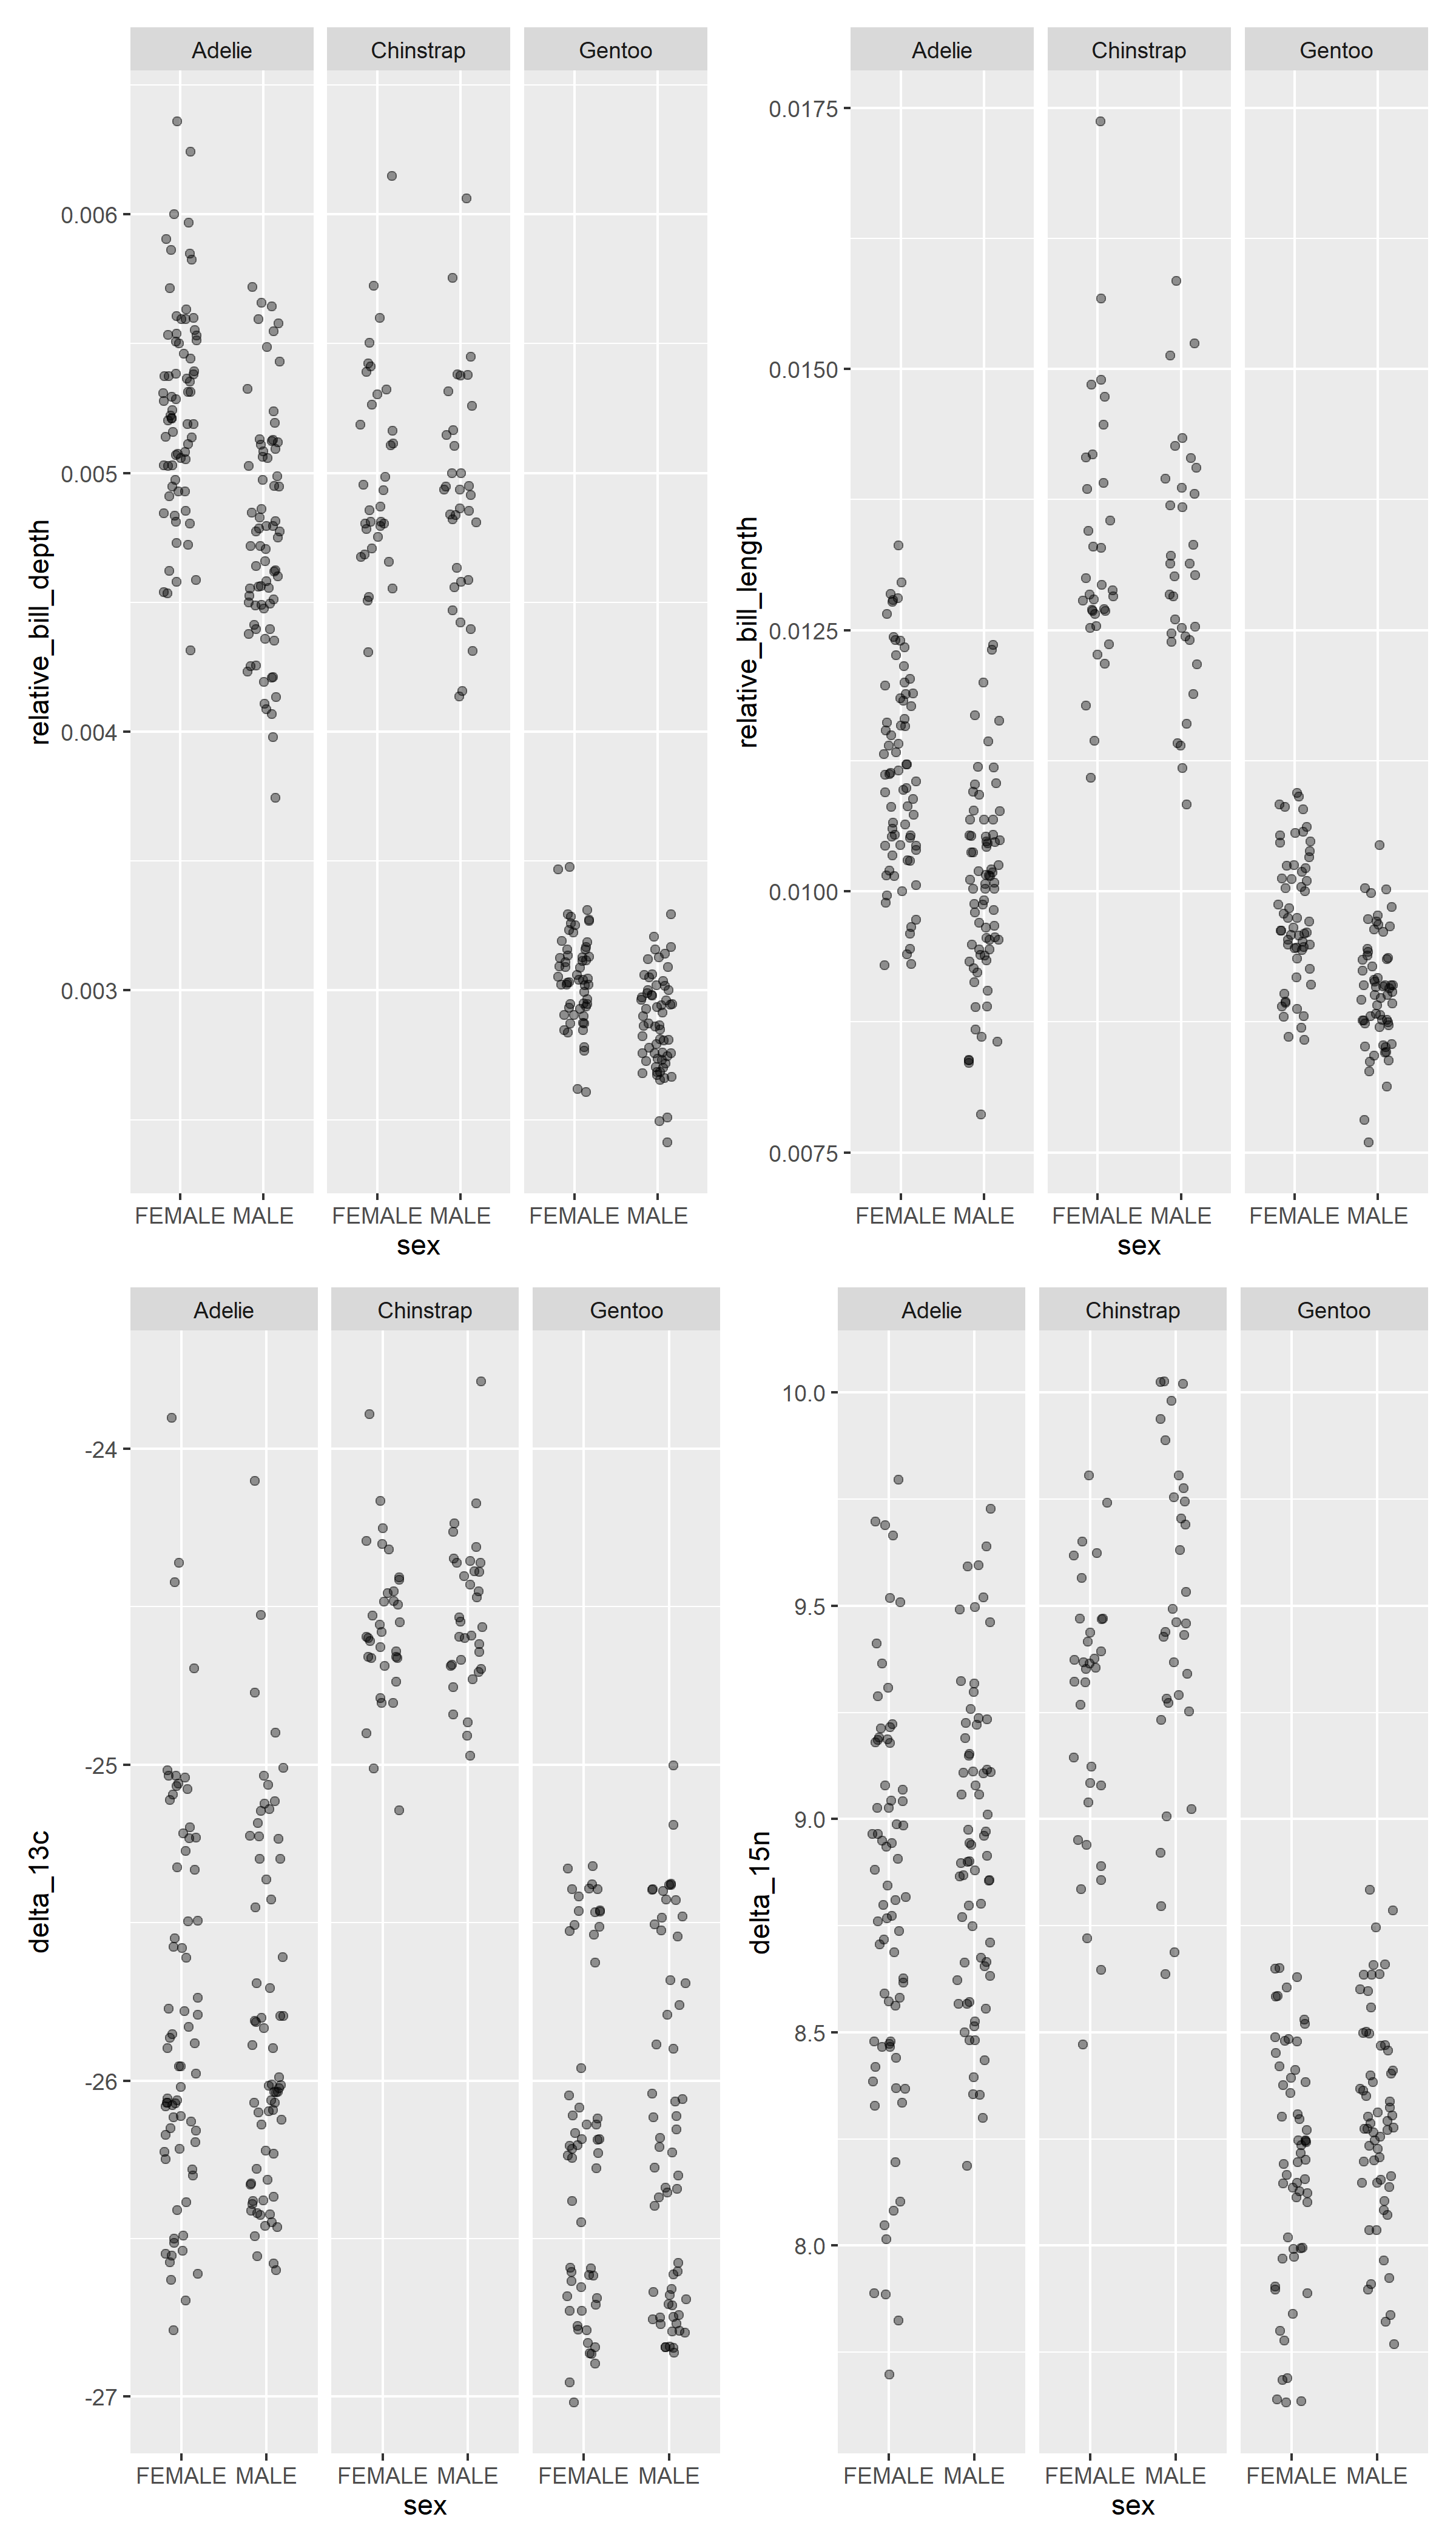
\includegraphics[width=0.8\linewidth]{images/summary} \caption{Difference in relative bill length and depth, and heavy carbon and nitrogen ratios, in male and female penguins from three different species - Adelie, Chinstrap and Gentoo}\label{fig:unnamed-chunk-111}
\end{figure}

\hypertarget{making-our-graphs-more-attractive}{%
\section{Making our graphs more attractive}\label{making-our-graphs-more-attractive}}

We will dive into making attractive ggplots in more detail later. But let's spend a little time now fixing some of the more serious issues with our figures.

The aim with making a good figure, is that it is:

\begin{itemize}
\item
  Accurate - the figure must present the data properly, and not distort or mislead
\item
  Beautiful - attractive figures will invite people to spend more time studying them
\item
  Clear - a good figure should be able to stand on its own - see the answer or insight without prompting from the text
\end{itemize}

There are lots of things we could change here, but we will stick with the basics for now. We will:

\begin{itemize}
\item
  Change the axis labels
\item
  Add some colours
\item
  Remove the grey background
\end{itemize}

\begin{Shaded}
\begin{Highlighting}[]
\NormalTok{penguins }\SpecialCharTok{\%\textgreater{}\%} 
    \FunctionTok{drop\_na}\NormalTok{(sex) }\SpecialCharTok{\%\textgreater{}\%} 
    \FunctionTok{ggplot}\NormalTok{(}\FunctionTok{aes}\NormalTok{(}\AttributeTok{x=}\NormalTok{sex, }
               \AttributeTok{y=}\NormalTok{relative\_bill\_depth,}
               \AttributeTok{colour=}\NormalTok{sex))}\SpecialCharTok{+}
    \FunctionTok{geom\_jitter}\NormalTok{(}\AttributeTok{position=}\FunctionTok{position\_jitter}\NormalTok{(}\AttributeTok{width=}\FloatTok{0.2}\NormalTok{), }
                \AttributeTok{alpha=}\FloatTok{0.4}\NormalTok{)}\SpecialCharTok{+}
  \FunctionTok{scale\_color\_manual}\NormalTok{(}\AttributeTok{values=}\FunctionTok{c}\NormalTok{(}\StringTok{"darkorange"}\NormalTok{, }\StringTok{"blue"}\NormalTok{))}\SpecialCharTok{+}
        \FunctionTok{facet\_wrap}\NormalTok{(}\SpecialCharTok{\textasciitilde{}}\NormalTok{species)}\SpecialCharTok{+}
  \FunctionTok{ylab}\NormalTok{(}\StringTok{"Relative culmen depth (mm)"}\NormalTok{)}\SpecialCharTok{+}
  \FunctionTok{xlab}\NormalTok{(}\StringTok{"Sex"}\NormalTok{)}\SpecialCharTok{+}
  \FunctionTok{scale\_x\_discrete}\NormalTok{(}\AttributeTok{labels=}\FunctionTok{c}\NormalTok{(}\StringTok{"Female"}\NormalTok{, }\StringTok{"Male"}\NormalTok{))}\SpecialCharTok{+}
  \FunctionTok{theme\_classic}\NormalTok{()}\SpecialCharTok{+}
  \FunctionTok{theme}\NormalTok{(}\AttributeTok{legend.position=}\StringTok{"none"}\NormalTok{)}
\end{Highlighting}
\end{Shaded}

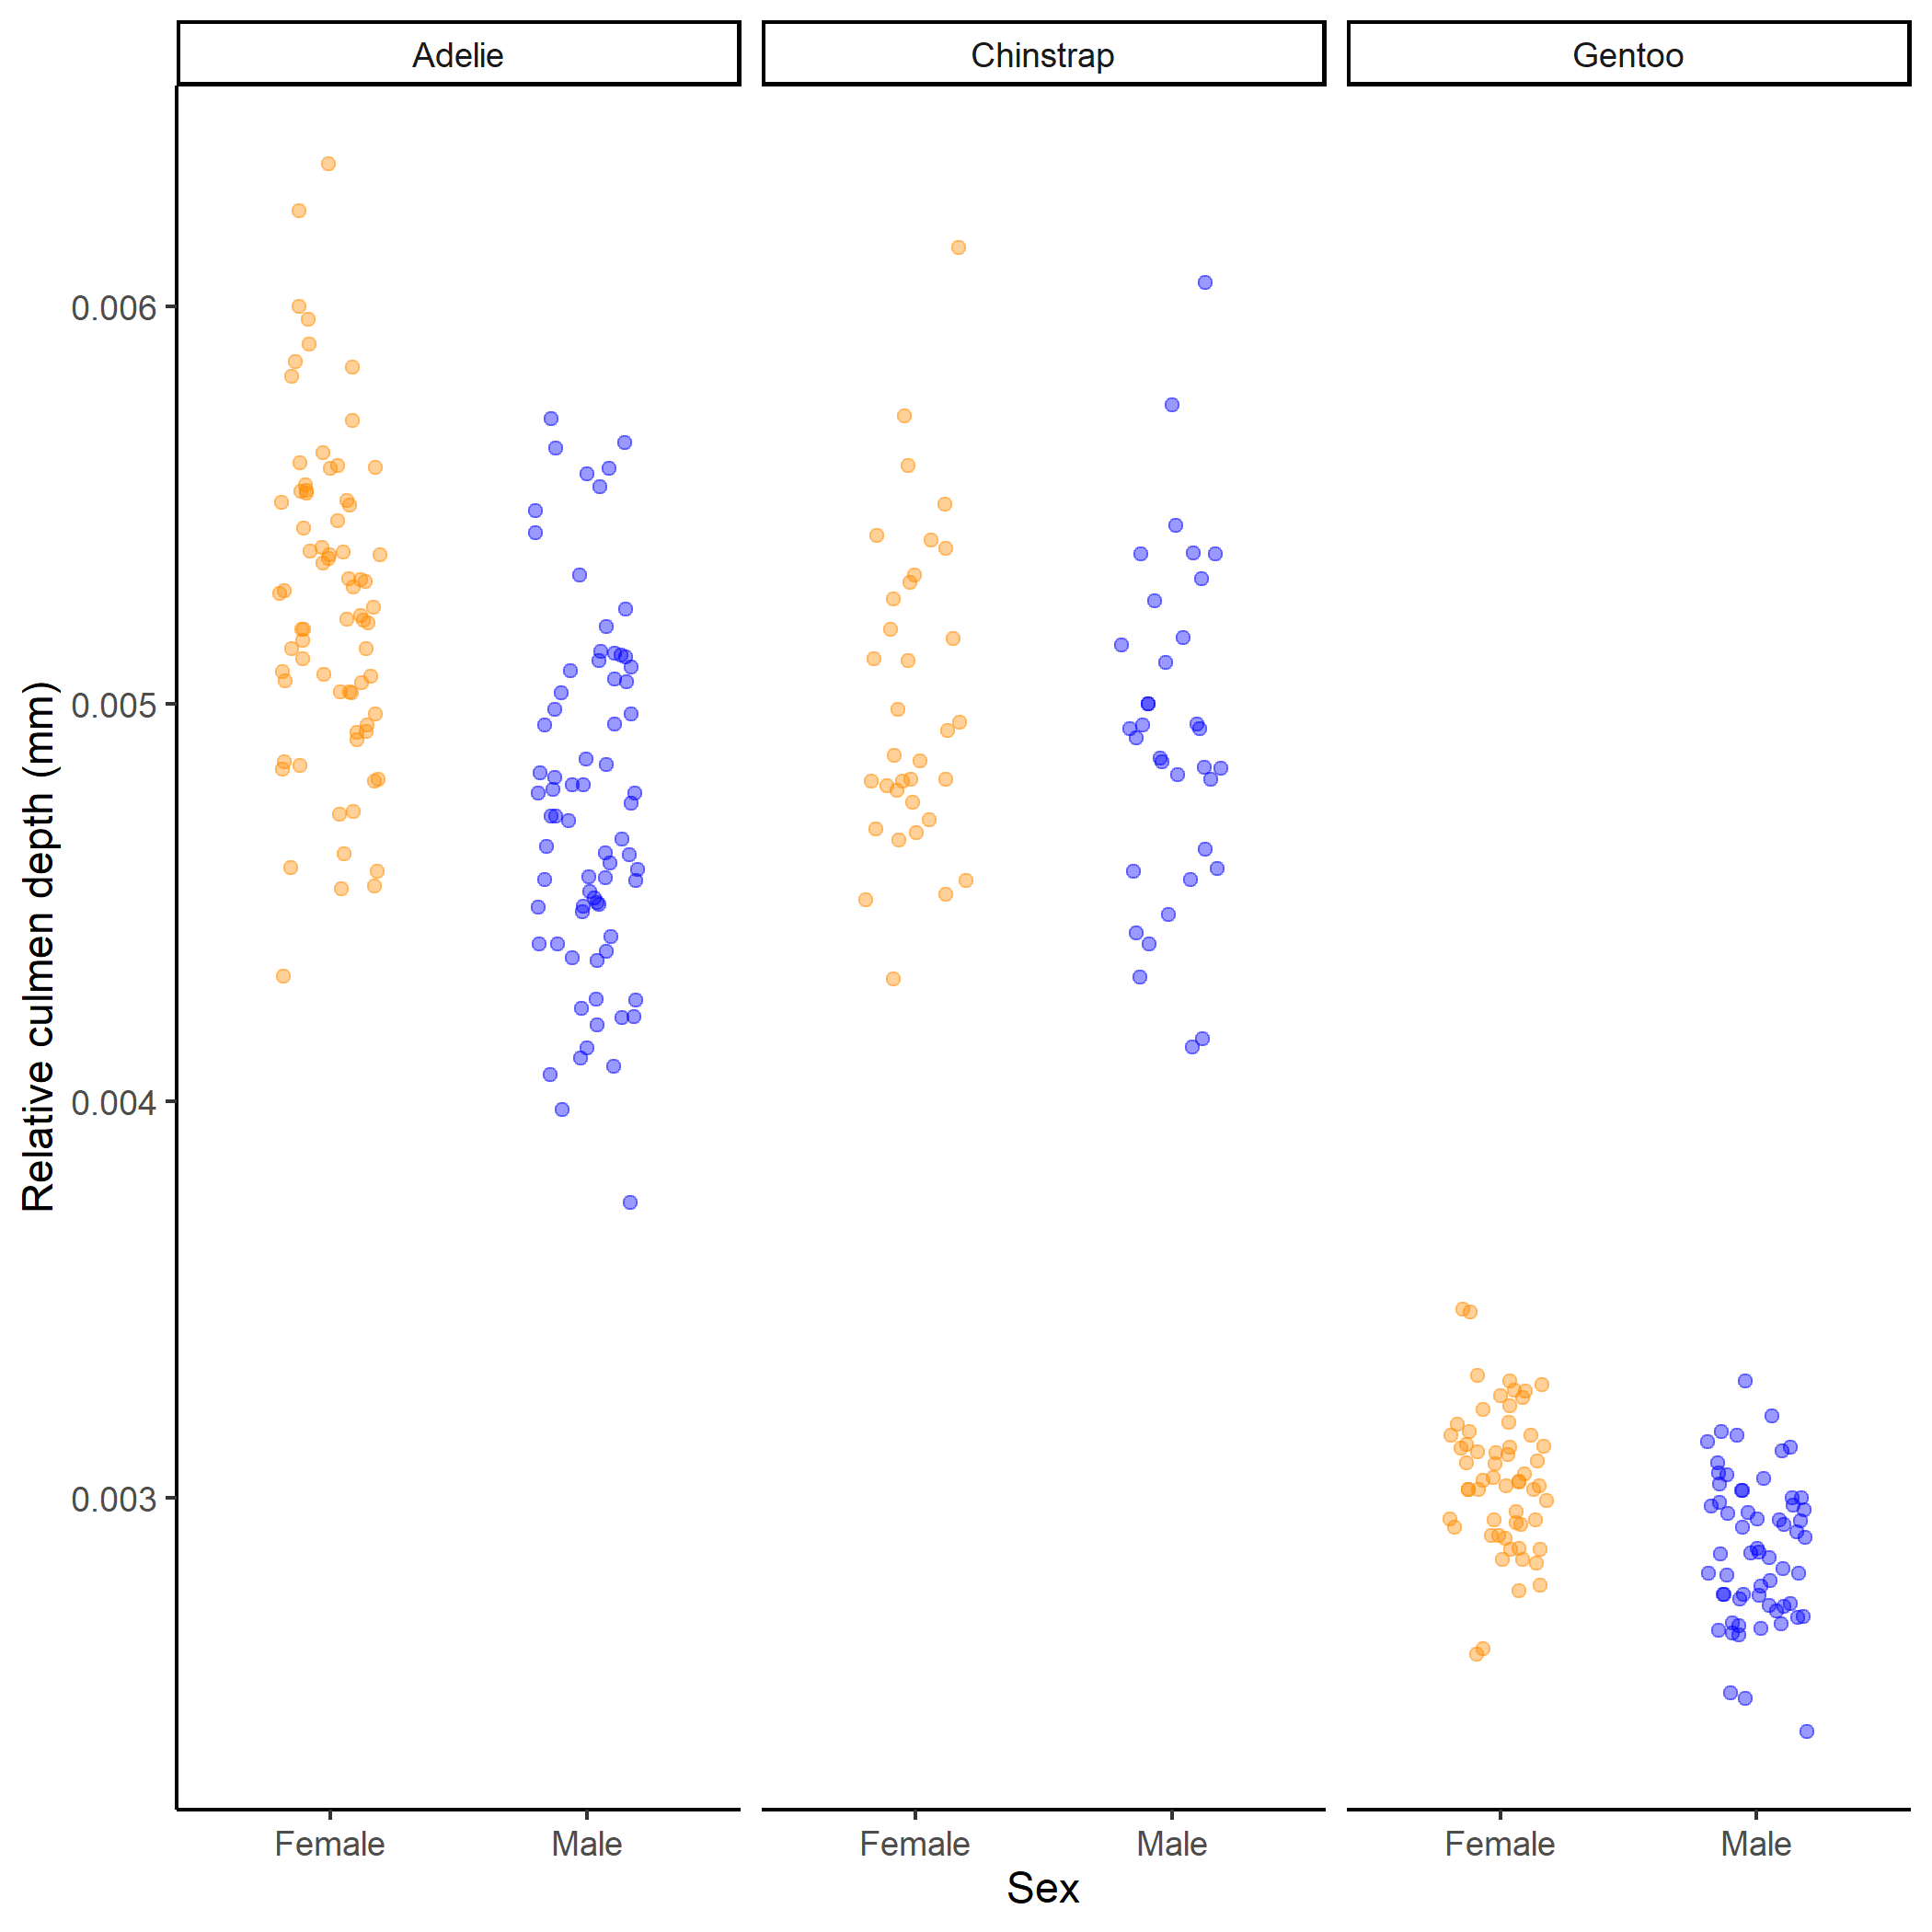
\includegraphics[width=0.8\linewidth]{images/final_figure_penguins}

\hypertarget{quitting-2}{%
\section{Quitting}\label{quitting-2}}

\begin{rmdwarning}
Make sure you have saved you script!
\end{rmdwarning}

\begin{rmdquestion}
Complete this week's Blackboard Quiz!
\end{rmdquestion}

*\href{https://www.rstudio.com/resources/cheatsheets/}{R Cheat Sheets}

  \bibliography{book.bib,packages.bib}

\end{document}
